% ============================================================================
%  main.tex -- Master thesis, University of Padua, Department of Information
%  Engineering (DEI), Master's Degree in Control Systems Engineering.
%
%  Master file for the DEI thesis template (class: DEIthesis).
%  Build (LaTeX toolchain required -- see DEI_COMPLIANCE.md):
%     pdflatex main
%     biber    main
%     pdflatex main
%     pdflatex main
%  or:  latexmk -pdf main
% ============================================================================

\documentclass{DEIthesis}

% ---- Frontespizio / thesis metadata -----------------------------------------
% Confirmed 2026-09-18 by the thesis author -- all fields below are final,
% not placeholders.
\title{Continual LoRA Merging for Class-Incremental Learning}
\author{Kasra Shahrampour}
\studentId{2106037}
\advisor{Prof. Pietro Zanuttigh}
% No co-supervisor: none was confirmed. No co-supervisor field exists in
% DEIthesis.cls (\advisor is the only advisor-type command it defines); if a
% co-supervisor is later confirmed, add a \coadvisor{...} command to
% DEIthesis.cls (mirroring \advisor) and render it beside \advisor in
% \maketitle.
\university{University of Padova}
\department{Department of Information Engineering}
\mastername{Control Systems Engineering}
% \academicYear is used ONLY for the title page's bottom defense-date line
% (DEIthesis.cls, \maketitle) -- confirmed by grep, no other use anywhere in
% the thesis. Set directly to the defense month/year rather than an
% academic-year range.
\academicYear{October 2026}

\begin{document}

% ---- Front matter order ----------------------------------------------------
% Title page / Abstract / blank / Acknowledgements / Contents / List of
% Figures / List of Tables / Preface / Chapter 1. Each \blankpage
% (DEIthesis.cls) is a single page with no header, footer, or printed page
% number. The Declaration of Originality (frontmatter/declaration.tex) is
% intentionally not included for now; its wording is pending the author's
% decision.
\frontmatter
\maketitle

\chapter*{Abstract}
\addcontentsline{toc}{chapter}{Abstract}

Rehearsal-free class-incremental learning with parameter-efficient
fine-tuning asks how a low-rank-adapted model can absorb a sequence of new
classes without storing past data and without catastrophically forgetting
what it already knows. This thesis studies two ways of organising LoRA
adaptation across such a sequence on a frozen CLIP ViT-B/16 backbone.
\emph{SimpleAvg} trains an independent, fixed-rank (rank-80) LoRA
specialist for each step and merges all specialists once, at the end, into
a single dense weight update; it is treated throughout as a strong
reference baseline rather than as a proposed contribution. \emph{RankExt}
instead grows one persistent, cumulative low-rank adapter across the
incremental sequence, adding a new rank block at each step while all earlier blocks
remain frozen but active, so that adaptation capacity is introduced
incrementally rather than specialist by specialist. Both strategies are
evaluated, with and without knowledge distillation and orthogonality-based
stabilisation, under a five-step/twenty-class-per-step class-incremental
protocol on CIFAR-100 as the primary benchmark, with CUB-200-2011
($5\times40$) as a second-dataset supporting evaluation, using paired
task-agnostic (open)
and task-oracle (restricted) evaluation to help distinguish what a model
still discriminates from what it can still express under output-space
competition with later steps.

SimpleAvg is unexpectedly strong on its own, reaching 75.16\% all-seen
accuracy with no auxiliary mechanism. Plain RankExt is far weaker, at
34.99\%, despite retaining high restricted accuracy, suggesting that
cross-step output-space competition contributes substantially to its poor
open performance while within-step discrimination remains comparatively
strong. This divergence between
restricted and open performance, which persists even where open accuracy
is poor, is a central diagnostic finding of this thesis. Auxiliary
stabilisation recovers most of RankExt's gap: combining knowledge
distillation with projected feature protection and a factor-space
orthogonality penalty brings its highest observed configuration to
70.76\% all-seen accuracy, 4.45 percentage points below the highest observed
SimpleAvg result (75.21\%). On CUB-200-2011 the same qualitative pattern
appears: plain SimpleAvg reaches 69.47\%, and the highest observed RankExt
configuration 63.43\%. The
comparison is not framed as a single winner-take-all contest: the central
question is how closely a persistent strategy that grows its adaptation
capacity incrementally can approach a strong, independently-trained
reference, and at what retention--plasticity cost. All headline benchmark
results are single-seed observations; multi-seed replication is identified
as a priority for confirming the findings.

\blankpage

\chapter*{Acknowledgements}
\addcontentsline{toc}{chapter}{Acknowledgements}

I would like to thank my supervisor, Prof.\ Pietro Zanuttigh, for his
guidance, feedback, and support throughout this thesis, and for the
freedom to pursue the experimental direction it eventually took.

I am also sincerely grateful to my co-supervisor, Eng.\ Leon Marx, for his
hands-on supervision of the
continual-learning experiments underlying this work: for the many
technical discussions, the help with experimental decisions, the careful
interpretation of results, and for repeatedly helping me refine the final
experimental direction when the path forward was not obvious.

Thank you to the friends and fellow students I met in Padova, whose
company, conversation, and encouragement made these years of study far
more enjoyable than they would otherwise have been.

Finally, my deepest thanks go to my family, especially my parents, for
their unwavering support and encouragement throughout my studies. None of
this would have been possible without them.


\tableofcontents
\listoffigures
\listoftables

\chapter*{Preface}
\addcontentsline{toc}{chapter}{Preface}

This project grew out of a simple interest in parameter-efficient continual
learning: given that low-rank adaptation already lets a large pretrained
model be fine-tuned cheaply for a single task, what happens when that
fine-tuning has to happen repeatedly, one incremental step after another,
without revisiting the data that came before? The central empirical
question that emerged from this starting point was not whether low-rank
adaptation works for continual learning in isolation, but how it should be
\emph{organised} across a sequence of incremental steps.

Two candidate organisations run through this thesis. The first,
\emph{SimpleAvg}, is deliberately simple: each step gets its own
independently trained, fixed-rank adapter, and their reconstructed dense
updates are combined once, at the end of the sequence, by arithmetic
averaging. It is treated throughout as a
reference point rather than as a proposed contribution in itself. The
second, \emph{RankExt}, is a persistent alternative in which a single
adapter is grown incrementally, one rank increment per step, with earlier
blocks left frozen but still active. One question that motivated much of
the experimental work reported here is how much of SimpleAvg's performance
a persistent, growing-rank strategy can recover, and what
stability--plasticity trade-off accompanies that recovery as auxiliary retention
mechanisms are added.

The resulting work is mainly empirical, comparative, diagnostic, and
ablative in character. It compares the two strategies under a common
protocol, examines where and why one struggles relative to the other, and
tests a number of auxiliary mechanisms and refinements against that
diagnosis. It does not claim to have invented low-rank adaptation, model
averaging, growing-rank continual adaptation, knowledge distillation, or
orthogonality-based regularisation; each of these building blocks is drawn
from existing practice and combined here for the specific purpose of this
comparison.

I hope the chapters that follow are useful not only for the specific
numbers they report, but for the diagnostic approach they take to reading
those numbers.


\mainmatter

% Exactly one blank page (no header, footer, or page number) follows each
% chapter. The class is oneside, so \cleardoublepage never adds a page of
% its own and no double blank pages can arise.
% ============================================================================
%  Chapter 1 -- Introduction
% ----------------------------------------------------------------------------
%  FORMAT CONVERSION of the six approved section drafts under
%  thesis_writing/chapter_1/section_1_1_v1.md .. section_1_6_v1.md, after
%  their full scientific/coherence/claim audit
%  (thesis_writing/chapter_1/chapter_1_full_audit_v1.md). Scientific prose is
%  preserved verbatim from the audited v1 drafts; only changes required for
%  valid LaTeX have been made (markdown heading/bold syntax, em-dashes,
%  citation commands, cross-references) -- see the itemised list below. The
%  audit's own MAJOR/MINOR/STYLE prose-revision recommendations are NOT
%  applied here; this pass is integration/formatting only.
%
%  Source-file mapping (kept unchanged as source/history, not further edited):
%    1.1 Background and Motivation  <- chapter_1/section_1_1_v1.md
%    1.2 Problem Statement          <- chapter_1/section_1_2_v1.md
%    1.3 Research Gap               <- chapter_1/section_1_3_v1.md
%    1.4 Research Questions         <- chapter_1/section_1_4_v1.md
%    1.5 Contributions              <- chapter_1/section_1_5_v1.md
%    1.6 Thesis Organization        <- chapter_1/section_1_6_v1.md
%
%  MECHANICAL CHANGES APPLIED (conversion only, no content change):
%    - Markdown "# 1.N Title" headings -> \section{Title} with a
%      \label{sec:ch1-...} slug, following Chapter 3's ch3-prefixed
%      labelling convention (Chapter 2 does not prefix; Chapter 1's section
%      names are generic enough -- "motivation", "contributions" -- that the
%      prefixed form was chosen to avoid any future collision).
%    - Markdown "**text**" -> \textbf{text} (RQ/contribution lead-ins),
%      matching the bold-lead-phrase convention already used in Chapter 2's
%      positioning section (e.g. "\textbf{The two adaptation strategies
%      (RQ1).}", chapter_2.tex around line 1002) and in Chapter 3's
%      \textbf{Procedure (...).} lead-ins.
%    - The four numbered contributions -> \begin{enumerate}...\end{enumerate}
%      with a \textbf{...} lead per \item -- \texttt{enumerate} is precedented
%      in this thesis (Chapter 3's two step-by-step procedures,
%      chapter_3.tex:974/1005); \texttt{itemize} is not used anywhere and was
%      not introduced here either.
%    - Literal "Section 1.N" / "Chapter N" cross-references -> \ref{} against
%      this chapter's own new sec:ch1-* labels and the existing ch:* chapter
%      labels defined by the DEI template, matching how Chapters 2/3
%      universally cross-reference (never a bare number). Section 1.6's
%      five paragraphs keep each chapter's descriptive title in prose
%      (\emph{...}) alongside \ref{} for the number -- content preserved,
%      only the number itself is now dynamic rather than hardcoded.
%    - Two Unicode em-dash-set-off clauses (1.3's and 1.4's closing/opening
%      sentences) -> LaTeX "---", unspaced, matching this thesis's dominant
%      em-dash convention (e.g. chapter_2.tex "baseline---the
%      independent-adapter-averaging case").
%    - "retention-plasticity" (hyphen, 6 occurrences across 1.1-1.3) ->
%      "retention--plasticity" (en-dash), matching Chapter 2's own rendering
%      of the identical term (chapter_2.tex:508, "retention--plasticity
%      comparison that motivates the primary research question") and the
%      cognate "stability--plasticity" (chapter_2.tex:87-88). This is the
%      one content-adjacent fix applied, and it is purely typographic
%      (identified as MINOR Issue 3 in the full-chapter audit and explicitly
%      named as a required special-character conversion for this pass); no
%      wording, claim, RQ, or contribution was altered.
%    - No other MAJOR/MINOR/STYLE item from chapter_1_full_audit_v1.md was
%      applied in THIS integration pass (Issues 1, 2, 4, 5, 6, 7 were left
%      open, deliberately, pending a separate scientific-revision pass).
%
%  MINIMAL REVISION PASS (2026-09-14, chapter_1_revision_report_v2.md):
%    applied the audit's MAJOR issue (1) and four of its five MINOR issues
%    (2, 4, 5, 6) to both this file and the corresponding v1 markdown
%    sources, keeping them synchronised; Issue 3 (retention--plasticity
%    dash) was already applied during the original integration pass above
%    and is unchanged here; Issue 7 (STYLE, Section 1.6 paragraph rhythm)
%    was reviewed and deliberately skipped as subjective -- see the
%    revision report for the full per-issue reasoning. No RQ, no
%    contribution's C-to-RQ mapping, no citation, and no chapter/section
%    structure was changed by this pass.
%
%  CITATION SYSTEM: biblatex, style=numeric-comp, backend=biber, configured
%    in DEIthesis.cls (line ~74). This is the ACTUAL configured style, not
%    the "style=authoryear" comment carried in Chapter 2/3's own headers
%    (a known-stale comment there, left untouched per instruction not to
%    modify Chapters 2/3 in this pass -- see
%    thesis_agent/reports/chapter_1_preparation_audit.md Section 20).
%    \parencite{key} and \textcite{key} are style-agnostic biblatex commands
%    and render as numeric, e.g. "[6]", under numeric-comp; they are used
%    directly here (not as temporary author-year placeholders) because every
%    key Chapter 1 cites was already confirmed to exist in references.bib
%    before drafting (thesis_agent/reports/chapter_1_preparation_audit.md
%    Section 13/17).
%
%  FORWARD REFERENCES: none left unresolved. Every "Chapter N" mention
%    resolves to the existing chapter labels defined elsewhere in this
%    project (ch:literature, ch:methodology, ch:experimental-setup,
%    ch:results, ch:discussion-conclusion); every "Section 1.N" mention
%    resolves to one of this chapter's own six new sec:ch1-* labels.
%
%  SUPERVISOR-FACING PRECISION REVISION (2026-09-23): scientific wording of
%    1.1-1.6 revised for consistency with the implemented experiments --
%    CIL framed as a subtype of continual learning; SimpleAvg defined as
%    independent per-step rank-80 adapters whose reconstructed dense updates
%    are arithmetically averaged once after the sequence; RankExt defined as
%    one persistent adapter with hard-frozen, still-active earlier rank
%    blocks; stabilisation (RQ2) made RankExt-focused; open/restricted
%    evaluation framed as primary measure + complementary diagnostic.
%    RQ4 and the protocol-depth contribution were REMOVED (three research-gap
%    components, three RQs, three contributions now). Figures 1.1 and 1.2
%    added from thesis_writing/pictures (baked-in captions cropped off; copies
%    under figures/chapter1/). The "four numbered contributions" note above
%    is historical.
% ============================================================================

\chapter{Introduction}
\label{ch:introduction}

\section{Background and Motivation}
\label{sec:ch1-motivation}

Large vision-language models pretrained on broad, weakly supervised
image-text corpora have reshaped how visual recognition systems are built.
Vision encoders trained under this paradigm, such as CLIP's, learn image
representations that transfer well across a wide range of downstream
recognition tasks without task-specific pretraining
\parencite{radford2021learning}. Such backbones offer an attractive starting
point for building a recognition system: rather than training a new model
per task from randomly initialised weights, a single strong,
general-purpose representation can instead be adapted to the task at hand.

Adapting a model of this scale separately for every downstream task is,
however, costly. Fully fine-tuning the entire backbone for each new task
requires storing a full copy of its parameters per task and repeating
expensive optimisation over the whole parameter set, a cost that scales
with the number of tasks supported. Parameter-efficient fine-tuning
addresses this problem directly: rather than updating all of a pretrained
model's weights, only a small number of additional parameters are
introduced and trained, while the backbone itself remains frozen. Low-rank
adaptation (LoRA) is a widely used instance of this idea, in which a
trainable low-rank update is added alongside a frozen weight matrix, so
that adaptation is expressed through a small number of additional
parameters rather than by modifying the backbone itself
\parencite{hu2021lora}. This substantially reduces the storage and compute
associated with adapting such a model to a new task, while retaining the
representational strength of the frozen backbone.

This picture implicitly assumes that the data required for a downstream
adaptation is available together, so that a single adaptation can be
trained and then deployed. The assumption becomes more restrictive in
continual learning, and more specifically in class-incremental learning,
where new classes arrive sequentially in disjoint groups. In the
rehearsal-free setting considered in this thesis, only the current step's
training data is available: examples from earlier steps are not retained
for replay, while classes belonging to later steps have not yet been
observed. Figure~\ref{fig:ch1-cil-setting} illustrates this setting.

\begin{figure}[htbp]
\centering
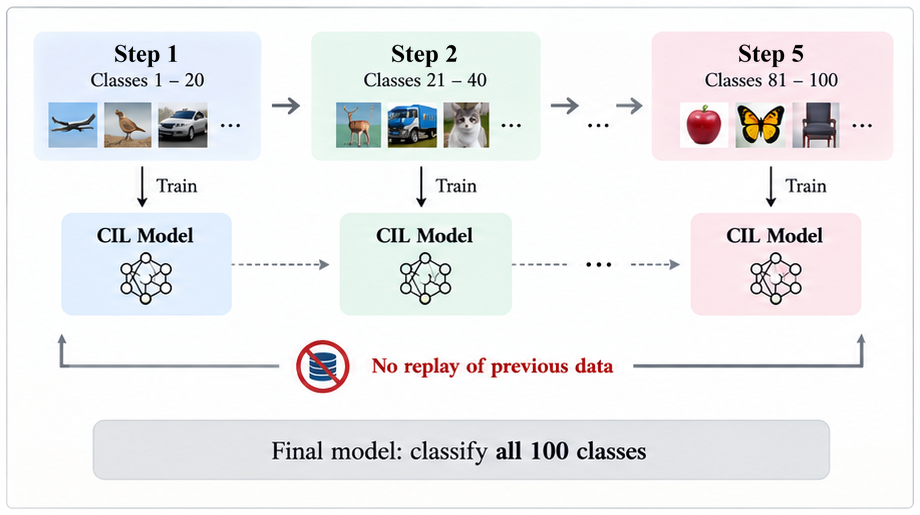
\includegraphics[width=0.85\textwidth]{figures/chapter1/ch1_rehearsal_free_cil_setting.png}
\caption[Rehearsal-free class-incremental learning setting]{Rehearsal-free
class-incremental learning setting used in this thesis. Disjoint groups of
classes arrive sequentially, no examples from earlier steps are replayed,
and the final model must classify all classes encountered across the
sequence. Conceptual redrawing based on the class-incremental learning
setting of \textcite{masana2020classincremental}.}
\label{fig:ch1-cil-setting}
\end{figure}

Training in this sequential manner exposes a central difficulty of
continual learning, catastrophic forgetting
\parencite{kirkpatrick2017overcoming}. In conventional sequential training,
updating parameters on newly arriving classes can degrade representations
or decision boundaries that support classes learned earlier. A continual
learner must therefore balance two competing requirements: it must remain
plastic enough to genuinely acquire new classes, while remaining stable
enough to retain competence on classes already learned. This tension,
commonly referred to as the retention--plasticity trade-off, is a central
challenge in class-incremental learning \parencite{delange2022continual}.

This difficulty is compounded under a rehearsal-free constraint, in which
no examples from earlier steps are stored and replayed alongside new data.
Rehearsal-based approaches can partially counteract forgetting by
re-exposing the model to past examples, but doing so requires retaining
raw data, which may be undesirable or infeasible for reasons of storage,
privacy, or deployment. Under a rehearsal-free constraint, information from
earlier steps must be preserved through retained model state rather than
through replay of the original training examples. This removes a direct
source of supervision for earlier classes and makes retention more
challenging.

Placing parameter-efficient adaptation in this sequential, rehearsal-free
setting raises a further, more specific design question. If each
incremental step produces its own low-rank adaptation, or extends a
shared one, how should the adaptations associated with different steps be
maintained, combined, or allowed to interact as training proceeds? Because
independently learned low-rank updates may interact when combined, the
integration rule itself can also influence continual-learning performance.
This thesis considers two structurally different answers. The first,
referred to here as SimpleAvg, trains an independent low-rank adapter at
each step, reconstructs the dense update induced by each adapter, and
combines these dense updates once, after the full incremental sequence, by
arithmetic averaging. The second, referred to here as RankExt, instead
maintains one persistent adaptation whose rank capacity is extended at each
step: new rank capacity is appended for the incoming classes, while
previously learned rank blocks remain active and are hard-frozen, so that
only the newly appended capacity is trained. Within this comparison,
SimpleAvg provides a reference based on independently trained per-step
adaptations, while RankExt tests how closely a single persistent model
whose adaptation capacity is introduced incrementally can approach that
reference. Combining independently trained components after the fact, and
extending a single adaptation's capacity over time, both build on broader
ideas in the literature reviewed in Chapter~\ref{ch:literature}; this
thesis examines the retention--plasticity behaviour each produces under one
shared rehearsal-free protocol. Figure~\ref{fig:ch1-integration-strategies}
summarises the two strategies.

\begin{figure}[htbp]
\centering
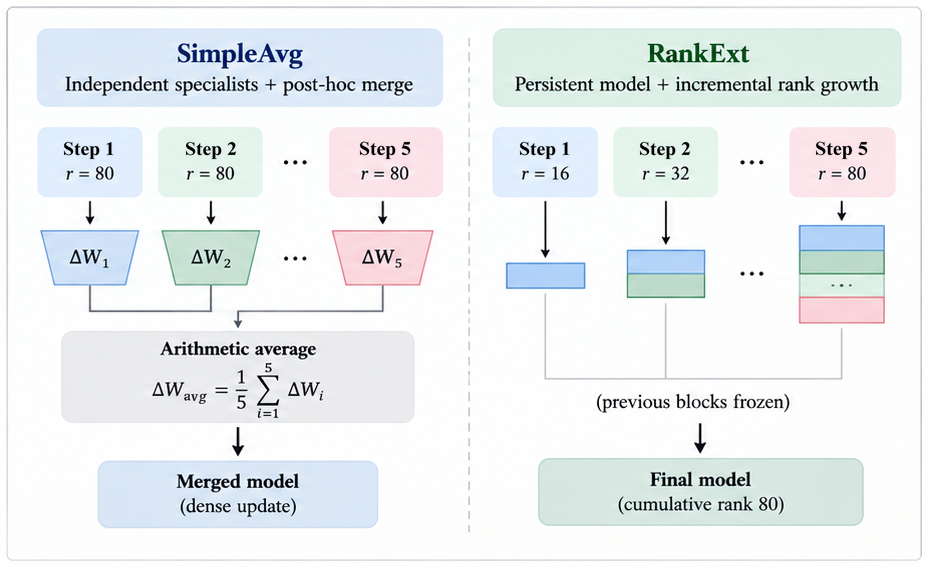
\includegraphics[width=0.9\textwidth]{figures/chapter1/ch1_simpleavg_vs_rankext.png}
\caption[The two LoRA integration strategies compared]{Overview of the two
LoRA integration strategies compared in this thesis. SimpleAvg trains
independent per-step adapters and combines their reconstructed dense
updates once after the sequence, whereas RankExt maintains a persistent
adapter whose capacity grows incrementally while previously learned blocks
remain frozen and active. The ranks shown correspond to the primary
$5\times20$ configuration. Original schematic.}
\label{fig:ch1-integration-strategies}
\end{figure}

Performance under either integration strategy can still be affected by
interference, although that interference arises differently in the two
families: independently learned updates may conflict when they are merged
in SimpleAvg, whereas newly introduced capacity in RankExt must coexist
with the frozen contributions retained from earlier steps. Additional
mechanisms are commonly introduced to limit such interference. Knowledge
distillation, in which a model is encouraged to match the outputs of an
earlier version of itself, and orthogonality-based regularisation, which
discourages a new update from overlapping with directions already used by
previous updates, are two such mechanisms examined in this thesis. Both are
established continual-learning tools; this thesis examines them primarily
within the persistent RankExt family, asking what role each plays there,
alone and in combination.
Section~\ref{sec:ch1-problem-statement} turns these observations into a
precise statement of the problem this thesis addresses.

\section{Problem Statement}
\label{sec:ch1-problem-statement}

The problem this thesis addresses can now be stated more precisely. A
pretrained visual backbone is adapted, using a parameter-efficient
mechanism, to a sequence of incremental steps, each introducing a disjoint
group of classes the model has not previously encountered. No training
examples from earlier steps are retained for replay: at each step, only
the classes introduced at that step are available for training. After
each incremental step, a class-incremental learner is expected to classify
over the cumulative set of classes encountered so far, rather than only the
classes introduced most recently. Under these constraints, the system must extend its competence to the new
classes of the current step while preserving its competence on classes
introduced at earlier steps, and it must do so without abandoning the
parameter-efficiency that motivated adopting a low-rank adaptation
mechanism in the first place. This is the retention--plasticity trade-off
introduced in Section~\ref{sec:ch1-motivation}, now situated concretely
within a rehearsal-free, parameter-efficient, class-incremental setting.

Because adaptation here is expressed through low-rank updates rather than
through full fine-tuning, a further, architecture-level problem arises.
Section~\ref{sec:ch1-motivation} raised this informally; formally, across
successive incremental steps, how should the resulting low-rank
adaptations be retained, combined, or extended? This thesis studies two
contrasting answers, treated as its two experimental families. Under the
first, SimpleAvg, an independent low-rank adapter is trained at each step;
the dense updates induced by these independently trained adapters are
reconstructed and combined once, after the full incremental sequence, by
arithmetic averaging. Under the second, RankExt, a single persistent
low-rank adaptation is maintained throughout, and its cumulative rank grows
over the sequence: previously learned rank blocks are retained and
hard-frozen while new rank capacity is appended at each step. Within this
comparison, SimpleAvg provides a reference based on independently trained
per-step adaptations, while RankExt tests how closely a single persistent
model whose adaptation capacity is introduced incrementally can approach
that reference. The precise mechanics of both families are given in
Chapter~\ref{ch:methodology}.

A further part of the problem is whether additional stabilisation can
improve the persistent RankExt family, where newly introduced capacity must
coexist with frozen earlier blocks. Two stabilisation mechanisms are
considered for this purpose: knowledge distillation, which encourages a
model to remain consistent with an earlier version of itself, and FactorOrth
regularization, an orthogonality-based penalty whose concrete formulation
is family-specific and which discourages a new update from occupying
directions already used by previous updates. This
thesis therefore examines knowledge distillation and FactorOrth
regularization within RankExt, while the corresponding SimpleAvg variants
are retained as supporting comparative evidence. Whether either mechanism,
or their combination, benefits RankExt is treated here as an open empirical
question rather than a settled one.

Finally, how retention is measured is itself part of the problem. A
class-incremental system's reported performance can differ substantially
depending on whether predictions are made freely over every class
encountered so far, or restricted to the classes belonging to one
already-identified incremental step \parencite{delange2022continual}.
This thesis therefore reports task-agnostic open evaluation as the primary
class-incremental measure and uses task-oracle restricted evaluation as a
complementary diagnostic of within-group discrimination and cross-group
competition.

Taken together, this thesis seeks to understand how the architecture used
to integrate successive low-rank adaptations, the stabilisation mechanisms
applied within the persistent RankExt family, and the conditions under
which retention is evaluated, jointly shape the retention--plasticity trade-off in
rehearsal-free class-incremental learning. Establishing where the existing
literature leaves this question open is the task of
Section~\ref{sec:ch1-research-gap}.

\section{Research Gap}
\label{sec:ch1-research-gap}

Section~\ref{sec:ch1-problem-statement} situated this problem in terms of
integrating successive low-rank adaptations, stabilising them against
interference, and evaluating the retention this produces, all within a
rehearsal-free class-incremental setting. The individual components
considered in this thesis build on established lines of work in
parameter-efficient fine-tuning, continual learning, knowledge
distillation, orthogonality-based regularisation, and model merging. What
is less directly characterised in the literature reviewed in
Chapter~\ref{ch:literature} is how these components interact when examined
within one shared, controlled rehearsal-free class-incremental framework.
In particular, this thesis focuses on the behaviour of a persistent
rank-extension strategy whose capacity grows incrementally while previously
learned rank blocks remain frozen and active, and uses independent per-step
adaptation with post-hoc averaging as a reference point against which that
behaviour can be interpreted.

The first component of this gap concerns integration architecture.
Persistent or growing low-rank adaptation has precedent in recent
continual-LoRA methods \parencite{wu2025sdlora,he2025cllora}, while the
combination of independently trained adaptations through weight averaging
is established in the model-merging literature
\parencite{wortsman2022model}. The literature reviewed in
Chapter~\ref{ch:literature} does not provide a directly matched comparison
between these two integration philosophies under the same rehearsal-free
class-incremental pipeline, with the same backbone, class partition, and
evaluation protocol. The closest methods reviewed in
Chapter~\ref{ch:literature} differ in architecture, training procedure,
evaluation protocol, or deployment assumptions, preventing a direct
like-for-like comparison of the two strategies considered here. This
comparison is especially informative for RankExt, since it asks how
closely a single persistent model whose adaptation capacity is introduced
incrementally can approach the reference provided by independently trained
per-step adaptations and post-hoc averaging.

The second component concerns stabilisation within the persistent RankExt
family. RankExt protects previously learned rank blocks structurally by
freezing them, but newly introduced capacity must still coexist with and
complement those frozen contributions. Knowledge distillation and
orthogonality-based regularisation are established continual-learning
mechanisms \parencite{li2016learning,wang2023orthogonal}: distillation
encourages the current model to remain consistent with the outputs of an
earlier model state, while orthogonality-based regularisation discourages
new low-rank updates from occupying directions already used by earlier
ones. Their contribution in this specific persistent growing-rank setting,
and particularly their interaction when combined, is not established by
the prior work reviewed here. The corresponding SimpleAvg variants are
retained as supporting comparative evidence rather than as the primary
focus of this question.

The third component concerns evaluation. Whether a class-incremental
model's predictions are drawn freely over every class seen so far, or
restricted to the classes of one already-identified step, is known to
shape the accuracy such a model reports, a sensitivity related to
task-recency effects previously documented in incremental classifier
competition \parencite{wu2019large}. The literature reviewed here provides
limited evidence on using these two evaluation modes as a paired
diagnostic on the same model and logits, read alongside the integration
and stabilisation choices above. The resulting open--restricted gap is
treated as a diagnostic indicator, not as a causal decomposition of
representational forgetting.

Taken together, these three components---integration architecture,
stabilisation within the persistent RankExt family, and evaluation
perspective---motivate the research questions that structure the remainder
of this thesis, stated precisely in
Section~\ref{sec:ch1-research-questions}.

\section{Research Questions}
\label{sec:ch1-research-questions}

The three central issues identified in
Section~\ref{sec:ch1-research-gap}---integration architecture,
stabilisation within the persistent RankExt family, and evaluation
perspective---are formulated below as the research questions this thesis
investigates. Each is stated as a comparison or characterisation to be
established empirically, not as a claim to be defended; how each is
answered is left to
Chapters~\mbox{\ref{ch:experimental-setup}--\ref{ch:discussion-conclusion}}.

\textbf{RQ1.} Under a rehearsal-free class-incremental learning protocol
with a LoRA-adapted CLIP ViT-B/16 backbone, how do persistent rank
extension (RankExt) and independent per-step adaptation followed by
dense-update averaging (SimpleAvg) compare in their trade-off between
old-class retention and new-class plasticity?

SimpleAvg provides the independent per-step reference for this
comparison, while RankExt tests how closely a persistent model with
incrementally introduced adaptation capacity can approach that reference
and what retention--plasticity trade-off accompanies doing so. RQ1 does
not presuppose a numerical outcome in favour of either family. Because the
two families are not matched in effective adaptation capacity, supporting
capacity analyses inform how this comparison is read, but capacity is not
treated as a separate research question.

\textbf{RQ2.} What roles do knowledge distillation and FactorOrth
regularization play in maintaining continual-learning performance within
the RankExt family?

RQ2 focuses on the persistent RankExt family specifically, examining how
its two stabilisation mechanisms behave, alone and in combination, rather
than assuming either is necessary or sufficient. How SimpleAvg responds to
the same mechanisms is treated as supporting comparative evidence, not as
the primary target of RQ2.

\textbf{RQ3.} How does task-agnostic open evaluation differ from
task-oracle restricted evaluation in assessing retention, and what does the
observed gap indicate about within-group discrimination and cross-group
classifier competition?

RQ3 is method-agnostic and diagnostic: it concerns how the evaluation
condition under which retention is measured affects what that measurement
can be taken to show, independently of which integration family or
stabilisation setting produced it. Together, these three questions define
the scope of the empirical investigation carried out in the remainder of
this thesis.

\section{Contributions}
\label{sec:ch1-contributions}

This thesis makes an empirical and analytical contribution to
rehearsal-free class-incremental learning with LoRA by establishing a
controlled framework for comparing alternative integration strategies,
analysing stabilisation within persistent rank extension, and diagnosing
retention under complementary evaluation conditions. The framework is
designed to separate the effects of integration architecture,
stabilisation, and evaluation perspective while keeping the backbone,
class-incremental protocol, and principal evaluation conditions
controlled. The main contributions of this thesis are:

\begin{enumerate}
\item \textbf{A controlled comparison of two LoRA integration strategies
   for rehearsal-free class-incremental learning.} The thesis compares
   independent per-step adaptation followed by dense-update averaging
   (SimpleAvg), which serves as the independent-per-step reference, with
   persistent rank extension (RankExt), in which a single adaptation grows
   incrementally while previously learned rank blocks remain frozen and
   active, within a common protocol using the same backbone, class
   partition, and evaluation framework. The contribution is the resulting
   characterisation of how each strategy trades old-class retention against
   new-class plasticity, and of how closely the persistent RankExt design
   approaches the SimpleAvg reference (RQ1), without presupposing that
   either family outperforms the other.

\item \textbf{A structured ablation of stabilisation mechanisms within the
   RankExt family.} The thesis systematically examines knowledge
   distillation, FactorOrth regularization, and their combination, as
   applied to RankExt, characterising the role each plays in maintaining
   continual-learning performance within this persistent growing-rank
   family (RQ2). The corresponding SimpleAvg variants are reported as
   supporting comparative evidence rather than as part of this
   contribution's primary scope.

\item \textbf{A paired open/restricted diagnostic evaluation of the
   trained models.} The thesis evaluates every trained continual model
   under two complementary conditions: task-agnostic open evaluation, which
   predicts over all classes seen so far, and task-oracle restricted
   evaluation, which predicts only among the classes of an
   already-identified incremental step. The gap between them is analysed
   as a diagnostic of cross-group classifier competition and of the
   conditions under which retention is measured (RQ3). It is not treated as
   a causal decomposition of forgetting, and neither perspective is claimed
   to be the true measure of retention.
\end{enumerate}

Together, these three contributions provide a structured analysis of LoRA
integration architecture, stabilisation within persistent rank extension,
and evaluation conditions in rehearsal-free class-incremental learning.
Section~\ref{sec:ch1-thesis-organization} describes how the remaining
chapters of this thesis are organised around them.

\section{Thesis Organization}
\label{sec:ch1-thesis-organization}

Chapter~\ref{ch:literature}, \emph{Literature Review}, situates the problem
introduced above within the broader continual-learning,
parameter-efficient fine-tuning, and model-merging literatures, reviewing
rehearsal-free methods, LoRA-based continual adaptation, distillation- and
orthogonality-based stabilisation, and recency-related evaluation effects,
before positioning this thesis relative to the closest existing work.

Chapter~\ref{ch:methodology}, \emph{Methodology}, formalises the
rehearsal-free class-incremental setting used throughout and defines the
two integration strategies compared in this thesis, SimpleAvg and RankExt,
together with knowledge distillation and FactorOrth regularization, whose
concrete formulation is family-specific, as stabilisation mechanisms, the classifier and calibration procedure applied to both
families, and the task-agnostic open and task-oracle restricted evaluation
protocols and retention metrics used to assess them.

Building on this framework, Chapter~\ref{ch:experimental-setup},
\emph{Experimental Setup}, specifies how it is instantiated for
experimentation: the dataset and primary class-incremental protocol under
which it is studied, the backbone and adaptation configuration, the
training and validation procedure, the resulting set of evaluated method
variants, and the reproducibility details underlying the reported
experiments.

Chapter~\ref{ch:results}, \emph{Results}, then reports and analyses the
empirical outcomes of this experimental setup, presenting the comparison
between SimpleAvg and RankExt, the ablation of stabilisation mechanisms
within RankExt, the paired open/restricted diagnostic evaluation, and
supporting capacity analyses where relevant.

Finally, Chapter~\ref{ch:discussion-conclusion}, \emph{Discussion and
Conclusion}, interprets these results in light of the research questions
and the research gap identified in this chapter, discusses the limitations
of the experimental design and the scope within which its findings should
be read, and closes with the conclusions this thesis supports and the
directions it leaves open for future work.

Taken together, this progression moves from the conceptual foundations and
literature positioning established here, through the methodological and
experimental definitions of Chapters~\ref{ch:methodology}
and~\ref{ch:experimental-setup}, to the empirical evaluation of
Chapter~\ref{ch:results} and the interpretation and conclusions of
Chapter~\ref{ch:discussion-conclusion}.

\blankpage
% ============================================================================
%  Chapter 2 -- Literature Review
% ----------------------------------------------------------------------------
%  FORMAT CONVERSION of thesis_writing/chapter_2/chapter_2_full_v2.md
%  (accepted working draft; passed code-truth, coherence, literature and
%  novelty audits). Scientific prose is preserved verbatim; only changes
%  required for valid LaTeX have been made (special-character escaping,
%  en/em dashes, inline math, quotation marks, citation commands,
%  cross-references).
%
%  Source assembly note (editorial metadata, not chapter prose):
%    Assembled draft (v2). Supersedes v1 after the final coherence +
%    code-truth audit (see chapter_2_truth_coherence_audit.md); six minor
%    edits applied -- FactorOrth reference wording, FactorOrth naming,
%    self-distillation wording, a 2.8->2.9 bridge, a de-duplicated sentence
%    in 2.9, and a P27 online-CIL qualifier. Citations are temporary
%    author-year tags in the source; here they resolve to biblatex keys
%    that map to thesis_agent/literature/literature_registry.jsonl.
%
%  CITATION SYSTEM: biblatex, backend=biber, configured in DEIthesis.cls.
%    UPDATED (final Ch.2 revision pass): the class now sets
%    style=numeric-comp (see DEIthesis.cls, "style=authoryear to
%    style=numeric-comp" note), so \parencite/\textcite both render as
%    numeric, comma-compressed bracketed citations (e.g. "[12]"), not the
%    author-year form this note originally described. The in-text commands
%    themselves are unchanged; only their rendered form differs from the
%    original assembly note below.
%    L2P (wang2022learning) and DualPrompt (wang2022dualprompt) are both
%    Wang et al. 2022; the source's generic "(Wang et al., 2022)" for
%    prompt-/prefix-tuning (Sections 2.3 and 2.4) is mapped to
%    wang2022learning (L2P), the canonical "learn to prompt for continual
%    learning" reference.
%
%  FORWARD REFERENCES: resolved. The source's literal "Chapter N" references
%    now use \ref{} against the chapter labels defined in the DEI template
%    (ch:methodology, ch:experimental-setup, ch:results, ch:discussion-conclusion).
%
%  EDITORIAL FIX (2026-09-06 LaTeX integration pass, Chapter 2/3 forward-
%    reference known issue): Section 2.4 previously said the adapter's
%    rank/scaling/target-modules were "specified in Chapter 4." Chapter 3
%    (now converted from chapter_3_full_v2.md, see chapters/chapter_3.tex)
%    is where these quantities are actually DEFINED (Section 3.2); Chapter 4
%    still holds the full experimental configuration. The sentence now
%    distinguishes the two: "defined in Chapter~\ref{ch:methodology}" /
%    "concrete experimental configuration ... in Chapter~\ref{ch:experimental-setup}."
%    No other wording in Chapter 2 was touched.
%
%  EQUATIONS: none as of the final Ch.2 revision pass. The forgetting-measure
%    display equation (former label eq:forgetting) was removed from this
%    chapter -- Section 2.10 now gives only the conceptual BWT/forgetting
%    distinction in prose and defers the exact formula to Chapter 3, which
%    still states it in full under its own label, eq:ch3-forgetting.
%
%  VISUALS (2026-09-06 pass; figure redrawn and one table removed in the
%    final Ch.2 revision pass): see chapter_2/chapter_2_visual_source_options.md
%    for external figures considered and NOT embedded, and
%    thesis_latex/ch2_ch3_latex_integration_audit.md for the original
%    candidate list and rationale.
%    fig:ch2-cl-taxonomy   -- original TikZ taxonomy tree (Section 2.1/2.5)
%    fig:ch2-lora-diagram  -- original TikZ LoRA schematic (Section 2.4),
%                             redrawn in the final revision pass into an
%                             explicit two-panel (training-time branch /
%                             merged inference form) layout; still an
%                             original diagram, not a reproduction of any
%                             external artwork (see the figure's own caption
%                             for provenance).
%    tab:ch2-eval-terminology -- terminology-mapping table (Section 2.9.2)
%    tab:ch2-related-work  -- REMOVED in the final Ch.2 revision pass (was:
%                             synthesis table before the positioning
%                             section). It duplicated the prose positioning
%                             already given in Section 2.11 and was judged
%                             too dense to earn its place; the prose
%                             positioning is preserved in full.
% ============================================================================

\chapter{Literature Review}
\label{ch:literature}

\section{Continual Learning: The Stability--Plasticity Problem}
\label{sec:continual-learning}

Continual learning, also referred to as lifelong or incremental learning,
concerns the training of a single model on a non-stationary stream of data,
in which tasks or groups of classes arrive in sequence and the learner
cannot revisit all of the earlier data \parencite{delange2022continual}. This
departs from the conventional supervised paradigm, where the entire
training distribution is available simultaneously and can be sampled
independently and identically throughout optimisation. Once that assumption
is removed, gradient-based training on newly arriving data tends to
overwrite the parameters responsible for previously acquired competence, a
failure mode known as catastrophic forgetting \parencite{kirkpatrick2017overcoming}.
Because the layers of a neural network are shared across every task,
updates that reduce the loss on the current data distribution can move
parameters away from regions that were favourable for earlier
distributions; forgetting is therefore most naturally understood as
interference in a shared parameter space rather than as the explicit
deletion of stored knowledge \parencite{kirkpatrick2017overcoming,delange2022continual}.

This interference exposes a fundamental tension. A model that is too rigid
retains earlier knowledge but cannot accommodate new classes or domains,
whereas a model that adapts without restraint acquires new competence at
the expense of the old. The continual-learning literature frames this as
the stability--plasticity trade-off: stability is the preservation of
previously learned representations, and plasticity is the capacity to
integrate new information \parencite{delange2022continual}. An effective continual
learner must reconcile the two, and most continual-learning methods can be
read as particular strategies for controlling where, over the course of
training, a model sits on this spectrum.

Continual-learning problems are commonly organised into scenarios that
differ in what changes between successive steps and in what information is
available at inference \parencite{masana2020classincremental,delange2022continual}. In
task-incremental learning, a task identifier is supplied at test time, so
the model need only discriminate among the classes belonging to the
identified task. In domain-incremental learning, the label space is fixed
while the input distribution shifts across steps. In class-incremental
learning (CIL), each step introduces a disjoint set of new classes, the
label space grows cumulatively, and no task identifier is available at
inference, so the model must discriminate among all classes encountered so
far. Class-incremental learning is generally regarded as the most demanding
of the three, because earlier classes must both be retained and placed in
direct competition with later ones under a single decision rule \parencite{masana2020classincremental}.
The present thesis operates entirely within the
class-incremental scenario; the benchmark conventions and protocol choices
that this entails are examined in Section~\ref{sec:cil}, and the remaining scenarios
are not pursued further.

Methods for mitigating forgetting in this setting are usually grouped into
three broad families \parencite{delange2022continual}. Replay-based, or
rehearsal-based, methods retain a subset of past examples, or synthesise
surrogates for them, and interleave these with current data so that earlier
distributions remain represented in the training signal. Regularisation-based
methods add a penalty that discourages changes to the parameters or outputs
deemed important for previous tasks, while storing no past data; Elastic
Weight Consolidation, which penalises movement of parameters identified as
important for earlier tasks, is the canonical instance \parencite{kirkpatrick2017overcoming}.
Parameter-isolation, or architecture-based, methods allocate
distinct parameter subsets to different tasks so that earlier capacity is
shielded from being overwritten by later updates. These families are not
mutually exclusive, and many methods combine elements of more than one. The
work in this thesis adopts a rehearsal-free constraint, meaning that no
past examples are retained in any form; the motivation for this constraint,
and a finer taxonomy of rehearsal-free techniques, are developed in Section~\ref{sec:rehearsal-free}.

Forgetting is not only a phenomenon to be mitigated but also a quantity to
be measured. Backward transfer (BWT) captures the average change in a
task's accuracy between the point at which it was first learned and the end
of training, so that negative backward transfer indicates forgetting
\parencite{lopezpaz2017gradient}. Related forgetting measures summarise, for
each earlier task, the gap between its best recorded performance and its
performance at the end of the sequence \parencite{chaudhry2018riemannian}. Such
measures also make explicit the complementary risk of excessive stability,
sometimes termed intransigence: a model that never updates does not forget,
but neither does it learn \parencite{chaudhry2018riemannian}. The precise definitions
adopted in this thesis, together with their relationship to raw accuracy on
the cumulative label space, are set out in Section~\ref{sec:cl-metrics}.

A final consideration, developed in Section~\ref{sec:recency-bias}, is that the accuracy a
class-incremental model reports on its earlier classes depends not only on
the quality of its internal representations but also on how the evaluation
is conducted. Whether a measured decline in earlier-class accuracy should
be read directly as representational forgetting is therefore an open
question at this stage, and one to which the discussion returns once
evaluation protocols have been introduced. The next section narrows the
focus from continual learning in general to the class-incremental setting
that all of the experiments in this thesis inhabit, and to the benchmark
conventions used to study it.

\section{Class-Incremental Learning: Setting and Benchmark Design}
\label{sec:cil}

Of the continual-learning scenarios distinguished in Section~\ref{sec:continual-learning}, this
thesis is concerned exclusively with class-incremental learning. In CIL, a
model is trained over a sequence of steps, and each step contributes a set
of classes that were not present in any earlier step. The classes
introduced at different steps are disjoint, and the set of categories the
model is expected to recognise grows cumulatively as steps accumulate, so
that after the final step the model must classify inputs across the union
of all classes seen so far \parencite{masana2020classincremental}. The literature also
refers to each such increment as a \enquote{task}; because CIL provides no separate
task structure at inference, this thesis uses the term \enquote{step} consistently
for an incremental class group and reserves no independent role for a task
identity.

The property that most sharply separates CIL from task-incremental learning
is what is available at test time. In task-incremental learning a task
identifier accompanies each input, so the model only has to discriminate
among the classes belonging to the identified task. CIL withholds this
identifier: predictions are made over the entire accumulated label space
through a single classification head, a regime commonly described as
single-head or global evaluation \parencite{masana2020classincremental,delange2022continual}. This
assumption makes the problem substantially harder, and increasingly so as
learning proceeds, because the model must not only represent each class but
also arbitrate between classes that were learned at different times, on
different data, and never jointly, under one decision rule. Each additional
step enlarges the pool of mutually competing categories.

It is in this arbitration that the catastrophic forgetting described in
Section~\ref{sec:continual-learning} becomes most visible. How much earlier information is available
while a step is trained depends on the method: some class-incremental
methods, iCaRL among them, reintroduce a stored subset of earlier examples,
whereas under a rehearsal-free constraint---the regime adopted in this
thesis---each step is trained on its new-class data alone, with no direct
signal preserving the earlier classes, so that the pressure on the shared
representation is correspondingly greater. In systems that classify through
a learned single-head linear layer, a well-documented symptom is that the
classifier becomes biased toward the classes added most recently,
predicting them disproportionately at inference \parencite{masana2020classincremental}; this
reflects that common design rather than a defining property of every
class-incremental method. The mechanisms underlying this bias, and the
techniques proposed to counter it, are examined in Section~\ref{sec:recency-bias}; for present
purposes it is enough to observe that single-head, classifier-based CIL is
particularly exposed to it.

Early class-incremental methods established both a set of algorithmic ideas
and a set of evaluation practices that remain influential. iCaRL \parencite{rebuffi2017icarl} is
representative: it retains a small set of stored examples from earlier
classes, adds a distillation term that encourages the updated model to
preserve its predecessor's responses on those classes, and classifies by
nearest mean of the stored exemplars in feature space rather than through a
learned linear layer. Later work kept the incremental framing while
revisiting each of these ingredients independently. Whether earlier
examples need to be stored at all is the question taken up in Section~\ref{sec:rehearsal-free}.

Empirical study of CIL depends on constructed protocols. A base
classification dataset is partitioned into groups of classes that are
presented in sequence, conventionally under a class ordering that is
randomised but then held fixed, so that reported results do not depend on a
favourable arrangement \parencite{rebuffi2017icarl,masana2020classincremental}.
Protocols differ along several axes: the total number of classes, the
number of incremental steps, whether the first step is larger than the
rest---for instance a substantial initial block followed by smaller
increments---and the number of classes introduced per step. Across the
literature the number of steps ranges from a handful to several dozen
\parencite{masana2020classincremental}. Because the outcome can depend on which classes
happen to arrive early, protocols are frequently evaluated over several
class orderings and the results averaged \parencite{masana2020classincremental}. Performance
is typically summarised in two complementary ways: by the accuracy over the
full accumulated label space measured after each step and averaged across
the sequence, often termed average incremental accuracy, and by the
accuracy after the final step \parencite{masana2020classincremental}. Retention specifically
is read from how the accuracy on an earlier step's classes evolves as later
steps are added; the formal measures used for this purpose are set out in
Section~\ref{sec:cl-metrics}. Image-classification datasets such as CIFAR-100 and subsets
of ImageNet are the usual testbeds.

One axis of protocol design deserves separate attention. For a fixed total
number of classes, the same class space can be divided into a few large
steps or into many small ones. This granularity---referred to here as
protocol depth---is not merely a matter of bookkeeping, because it governs
how many times the model is updated over the course of training and how
much new information each update introduces, both of which plausibly bear
on how much is forgotten. The literature on whether protocol depth has a systematic effect on
forgetting is reviewed in Section~\ref{sec:protocol-depth}. The concrete protocol used in
this thesis, together with the dataset, the class ordering, and the
training configuration, are specified in Chapter~\ref{ch:experimental-setup}. The remainder of
Chapter~\ref{ch:literature} turns to the strategies that have been proposed for limiting
forgetting under the conditions set out above, beginning in Section~\ref{sec:rehearsal-free}
with those that operate without storing any past data.

\subsection{Protocol Depth and Task Granularity}
\label{sec:protocol-depth}

The way a benchmark's class space is divided into incremental steps is not
a neutral formatting decision but an experimental factor in its own right.
Surveys of the area report a broadly consistent pattern: for a fixed
dataset, dividing it into more, and therefore smaller, increments tends to
lower final accuracy and increase measured forgetting \parencite{masana2020classincremental,delange2022continual}.
Plausible explanations include the larger number of sequential updates,
each fitted to a narrower slice of the label space, and the fewer occasions
on which different classes are seen together; which of these dominates is
not settled, and the classifier-competition component is taken up in
Section~\ref{sec:recency-bias}.

Protocol depth, as the term introduced in Section~\ref{sec:cil} is used
here, refers to the number of incremental steps into which a fixed total
class space is partitioned; a controlled protocol-depth comparison would
hold the total class count and the final adaptation capacity fixed while
varying the partition depth. This is narrower than task granularity in the
general sense, which also covers how semantically coarse or fine the
categories themselves are, and distinct again from curriculum or
class-ordering effects, which concern the sequence in which classes are
presented and can matter even when depth is held fixed.

Comparatively little prior work isolates depth through a controlled
design. A recent study \cite{alyamac2026evaluating} asks whether task
granularity affects catastrophic forgetting, but does so by comparing
semantic curriculum orderings---coarse-to-fine, fine-to-coarse, and
flat---over a small subset of classes with a single regulariser (EWC), so
granularity and ordering vary together and the number of steps is not
isolated as an independent variable. A comparison that varies step count
alone, with a fixed method and matched capacity, is less directly
examined, particularly for capacity-growing adapter architectures of the
kind introduced in Section~\ref{sec:lora-cl}.

Protocol depth is not a research question of this thesis. All main
results use the single primary five-step protocol ($5\times20$,
Chapter~\ref{ch:experimental-setup}); only one secondary $4\times25$
diagnostic is reported (Section~\ref{sec:ch5-ablation}), which is not
sufficient to characterise protocol-depth effects systematically. Protocol
depth therefore bounds how far the results reported here can be
generalised, and a controlled protocol-depth study is identified as future
work in Section~\ref{sec:ch6-future-work}.

\section{Rehearsal-Free Continual Learning}
\label{sec:rehearsal-free}

The most direct defence against forgetting is to keep some of the earlier
data. Replay, or rehearsal, stores a subset of past examples---or trains a
generator to produce surrogates---and mixes them into each new step's
training, so that the earlier distributions continue to shape the loss.
Across the continual-learning benchmarks surveyed by \cite{delange2022continual},
replay-based methods are among the most effective, and the
canonical class-incremental method iCaRL \parencite{rebuffi2017icarl}, discussed
in Section~\ref{sec:cil}, depends on a stored exemplar set. Retaining raw training
examples, however, has costs: it consumes a memory budget that grows with
the number of classes, and in many settings the earlier data cannot
lawfully or practically be kept. These considerations motivate
rehearsal-free, or exemplar-free, continual learning, in which raw examples
from previous steps are not retained for later training. This should not be
conflated with a fully memory-free setting, since a rehearsal-free learner
may still preserve model parameters, previous checkpoints, or compact
auxiliary statistics. This thesis adopts the rehearsal-free constraint
throughout.

Rehearsal-free methods are commonly grouped into a small number of
families, most of them refinements of the mitigation categories introduced
in Section~\ref{sec:continual-learning}. Regularisation-based methods add a penalty that discourages
changes to weights or outputs important for earlier steps; Elastic Weight
Consolidation \parencite{kirkpatrick2017overcoming} is the standard reference point.
Parameter-isolation, or architecture-based, methods give different steps
their own parameters, so that earlier capacity is structurally protected
rather than merely regularised. Distillation-based methods constrain the
updated model's outputs to remain close to those of a frozen copy of its
earlier self; Learning without Forgetting \parencite{li2016learning} is the
canonical example, and this mechanism is examined in Section~\ref{sec:kd}. A fourth
line of work leaves the representation untouched and instead re-balances the
final classifier after training to counteract its skew toward recent
classes, which is taken up in Section~\ref{sec:recency-bias}. The families are not exclusive,
and competitive systems usually combine several. Removing the memory buffer
generally costs some accuracy relative to replay-based methods \parencite{delange2022continual};
rehearsal-free research is in large part concerned with
narrowing that gap by making better use of the frozen representation and by
constraining more tightly what each step is permitted to change.

Much recent rehearsal-free work for class-incremental learning has
converged on a common template: a large pretrained model is frozen, and
only a small set of additional parameters is trained per step---whether
input-space prompts \parencite{wang2022learning} or low-rank weight updates
\parencite{wang2023orthogonal,liang2024inflora}. This
keeps the pretrained representation intact, bounds the trainable-parameter
budget, and removes any need to store data from earlier steps. The
adaptation mechanism used in this thesis follows the same template; it is
introduced in Section~\ref{sec:peft-lora}, and its use specifically for continual learning---%
including the design space of approaches that grow, merge, or route such
modules across steps---is the subject of Section~\ref{sec:lora-cl}.

\section{Parameter-Efficient Fine-Tuning and Low-Rank Adaptation}
\label{sec:peft-lora}

Adapting a large pretrained model by fine-tuning all of its weights is
expensive in computation and storage, and in a continual setting it has a
further drawback: every update moves the entire shared representation,
which is precisely what needs to be protected. Parameter-efficient
fine-tuning (PEFT) avoids this by freezing the pretrained weights and
training only a small number of additional or reparameterised parameters
\parencite{houlsby2019parameter}. Several PEFT families exist: bottleneck adapters
insert small trainable modules between the frozen layers \parencite{houlsby2019parameter};
prompt- and prefix-tuning prepend learnable vectors to the input or
to intermediate activations \parencite{wang2022learning}; and low-rank adaptation
modifies the existing weight matrices through an additive low-rank term
\parencite{hu2021lora}. This thesis uses low-rank adaptation exclusively; no
other PEFT family was implemented or compared, which is a deliberate
scoping decision rather than an empirical ranking.

Low-rank adaptation (LoRA) rests on the observation that the weight change
induced by adapting a model to a new task tends to have low effective rank
\parencite{hu2021lora}. For a frozen weight matrix, LoRA keeps that matrix fixed
and learns an update expressed as the product of two thin matrices whose
shared inner dimension---the rank---is far smaller than the dimensions of
the original weight; a scalar factor rescales the update's contribution.
The number of trainable parameters is therefore a small fraction of the
full matrix. Because the learned low-rank update has the same shape as the
original weight matrix, standard LoRA updates can be merged into the base
weights after training, avoiding a separate adapter branch at inference;
unlike inserted adapters, this adds no extra layers. Continual-learning
architectures built on LoRA differ, however, in how far they retain this
property. In transformer models the update is usually applied to the
projection matrices of the attention mechanism, which is also the choice
made here. Figure~\ref{fig:ch2-lora-diagram} summarises this mechanism
schematically.

\begin{figure}[htbp]
\centering
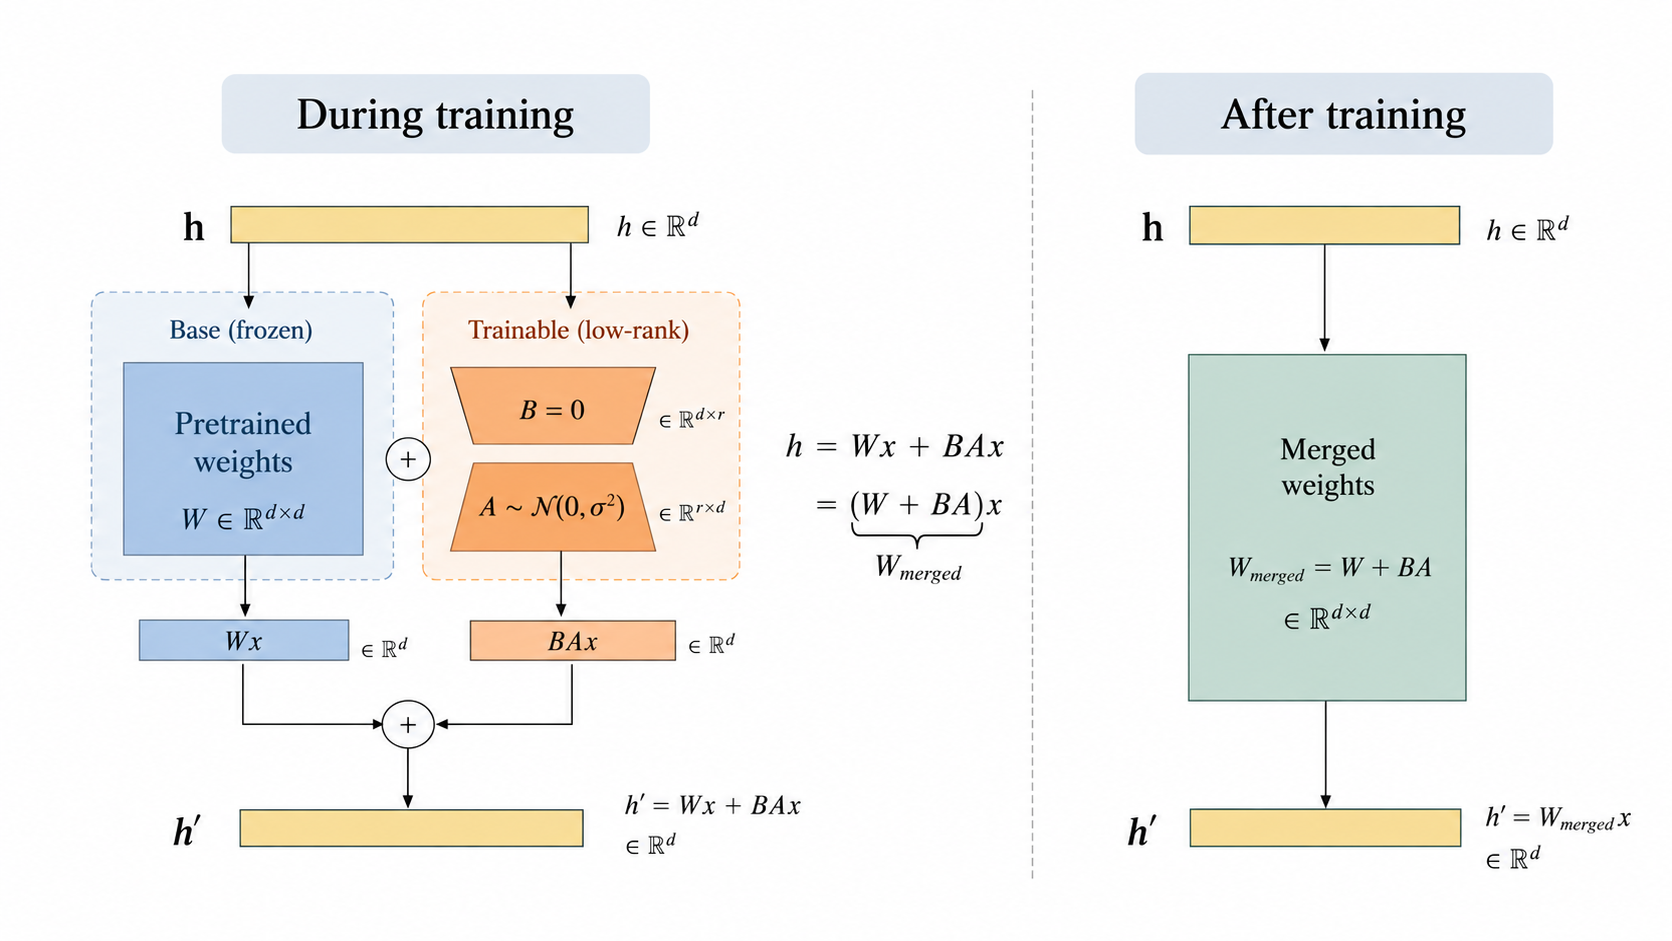
\includegraphics[width=0.85\textwidth]{figures/lora_training_inference_schematic.png}
\caption[Low-rank adaptation (LoRA) schematic]{Schematic illustration of
LoRA during training and after weight merging. During training, the
pretrained weight matrix $W$ remains frozen while the low-rank factors $A$
and $B$ learn the additive update $BA$. After training, the update is
merged into the base matrix as $W_{\mathrm{merged}} = W + BA$, so inference
uses a single weight matrix without a separate LoRA branch. Conceptual
redrawing based on \textcite{hu2021lora}.}
\label{fig:ch2-lora-diagram}
\end{figure}

The pretrained model to which these adapters are attached is the vision
encoder of CLIP \parencite{radford2021learning}, a Vision Transformer \parencite{dosovitskiy2021image}.
CLIP is trained on a large collection of image--text pairs
and produces visual features that transfer well across recognition tasks,
which makes it a strong frozen starting point; its text encoder plays no
role in this thesis, and classification is performed by a trained linear
layer rather than by matching against text prompts. As with the choice of
PEFT family, no alternative backbone was evaluated, and this
single-backbone scope should be borne in mind when interpreting later
results. Refinements of LoRA that quantise the frozen weights, decompose
the update differently, or allocate rank adaptively have since been
proposed; none is used here. The adapter---its rank, its scaling, and the
modules it is applied to---is defined in Chapter~\ref{ch:methodology}, and its
concrete experimental configuration is specified in Chapter~\ref{ch:experimental-setup}.
How low-rank adaptation is used as the vehicle for continual
learning, rather than for one-off task adaptation, is the subject of
Section~\ref{sec:lora-cl}.

\section{Continual Learning with LoRA-Based Adaptation}
\label{sec:lora-cl}

Using low-rank adaptation for a sequence of steps rather than for a single
task confines all adaptation to a small and structurally regular set of
parameters. This makes the composition question explicit---how should the
per-step updates be combined?---and the literature offers three broad
answers.

The first keeps separate per-step parameters and selects or combines them
at inference. The prompt-based methods L2P \parencite{wang2022learning} and
DualPrompt \parencite{wang2022dualprompt} are the prominent instances: they attach a
set of learnable prompt vectors to a frozen backbone and retrieve the
relevant ones for each input through a learned key--query mechanism that
needs no task label at test time, with DualPrompt separating task-shared
from task-specific prompts. These methods operate in input space rather
than weight space and are noted here as a sibling family rather than a
comparison point.

The second strategy trains an adapter independently at each step and merges
the results into a single set of weights afterwards; this is the subject of
Section~\ref{sec:model-merging}.

The third maintains a persistent low-rank component that is extended or
updated as steps arrive. SD-LoRA \parencite{wu2025sdlora} appends a new low-rank
direction pair at each step, freezing the earlier directions while leaving
their magnitudes trainable. CL-LoRA \parencite{he2025cllora} combines a shared
adapter that is updated throughout with per-task adapters that are frozen
after their step, re-running each task's adapter at inference so that its
inference cost grows with the number of steps. InfLoRA \parencite{liang2024inflora}
restricts each step's update to a subspace chosen so as not to interfere
with earlier tasks. Merge-before-Forget \parencite{qiao2025merge}, in the
language domain, consolidates each step into one rank-capped adapter by
merging before the next step begins. The broader literature therefore
establishes persistent, expandable, and selectively composed low-rank
adaptation as an active continual-learning design space, whose members
differ substantially in whether past components are frozen, retained
separately, continuously updated, or merged. It is this design space, not
any single architecture within it, that is well established.

This thesis compares two points in this space: a persistent adapter whose
rank is extended step by step, termed RankExt, and a set of independently
trained per-step adapters combined by simple averaging, termed SimpleAvg;
both are defined in full in Chapter~\ref{ch:methodology}. RankExt belongs to the
growing-adapter family described above and shares its overall shape; its
distinguishing features are at the level of mechanism rather than concept.
The parameters contributed by earlier steps are hard-frozen with no
remaining trainable degrees of freedom, in contrast to SD-LoRA's trainable
magnitudes or CL-LoRA's continuously updated shared component; interference
between old and new parameters can be further limited by a loss term that
penalises their overlap (Section~\ref{sec:orthogonality}) and, optionally, by self-distillation
from an earlier checkpoint of the model (Section~\ref{sec:kd}). Inference
uses a single persistent adapter and requires no per-step routing or
repeated step-specific forward passes; however, the adapter's parameter and
computation footprint grows with its cumulative rank. SimpleAvg,
by contrast, is included as a deliberately simple merging baseline---the
independent-adapter-averaging case, treated in Section~\ref{sec:model-merging}---and is not put
forward as a new method. The purpose of pairing them is the
retention--plasticity comparison that motivates the primary research
question, not the introduction of either as a novel architecture.
Figure~\ref{fig:ch2-cl-taxonomy} places this pair, and the broader
LoRA-based continual-learning design space around them, within the
taxonomy developed over the course of this and the preceding sections.

\begin{figure}[htbp]
\centering
\resizebox{\textwidth}{!}{%
\begin{tikzpicture}[
  every node/.style={font=\small, align=center},
  root/.style={draw, thick, rounded corners, minimum height=0.9cm, minimum width=3.2cm, fill=black!5},
  fam/.style={draw, thick, minimum height=0.9cm, minimum width=3.6cm},
  leaf/.style={draw, minimum height=0.8cm, minimum width=3.6cm},
  edge from parent/.style={draw, -{Latex[length=1.8mm]}},
  level 1/.style={sibling distance=4.1cm, level distance=1.6cm},
  level 2/.style={sibling distance=3.9cm, level distance=1.7cm},
  level 3/.style={sibling distance=3.9cm, level distance=1.7cm},
]
\node[root] {Continual learning\\\footnotesize(Section~\ref{sec:continual-learning})}
  child { node[fam] {Replay-based} }
  child { node[fam] {Regularisation-based\\\footnotesize (e.g.\ EWC)} }
  child { node[fam] {Parameter-isolation /\\architecture-based} }
  child { node[fam] {Pretrained backbone,\\PEFT-based\\\footnotesize(Section~\ref{sec:peft-lora})}
    child { node[leaf] {LoRA-based adaptation\\\footnotesize(Section~\ref{sec:lora-cl})}
      child { node[leaf, minimum width=3.4cm] {Selected/composed\\per-step prompts\\\footnotesize(L2P, DualPrompt)} }
      child { node[leaf, minimum width=3.4cm, fill=black!5] {Independent-per-step,\\merged post-hoc\\\footnotesize(\textbf{SimpleAvg}; Section~\ref{sec:model-merging})} }
      child { node[leaf, minimum width=3.4cm, fill=black!5] {Persistent,\\growing-rank\\\footnotesize(\textbf{RankExt}; SD-LoRA,\\CL-LoRA, InfLoRA)} }
    }
  };
\end{tikzpicture}%
}
\caption[Continual-learning taxonomy]{Taxonomy of continual-learning
strategies as developed in this chapter. The three families on the left are
introduced in Section~\ref{sec:continual-learning}; the rehearsal-free,
pretrained/PEFT-based template (Sections~\ref{sec:rehearsal-free}--\ref{sec:peft-lora})
and the three strategies for organising LoRA parameters across an
incremental sequence (Section~\ref{sec:lora-cl}) are drawn as its own
branch rather than as a fourth sibling of the original three, since it cuts
across them (most concretely, it is a rehearsal-free specialisation of the
regularisation- and parameter-isolation-based families). Shaded leaves mark
the two strategies compared in this thesis. Original synthesis figure; no
single source in the literature presents this exact taxonomy.}
\label{fig:ch2-cl-taxonomy}
\end{figure}

\section{Model Merging}
\label{sec:model-merging}

Model merging combines the weights of several independently trained
networks into a single set of parameters, without further training and
without keeping the individual models at inference. The idea was
popularised by model soups \parencite{wortsman2022model}, which showed that
averaging the weights of models fine-tuned from a shared initialisation
with different hyperparameters can improve accuracy at no inference cost.
Task arithmetic \parencite{ilharco2023editing} generalised the operation: each
fine-tuning run is summarised by a task vector, the difference between the
fine-tuned and the base weights, and these vectors can be added to combine
capabilities or negated to remove them.

The quality of a merge is governed by interference between the
contributions being combined. When two updates disagree about the sign or
magnitude of a change to the same parameter, averaging them partially
cancels both, and the merged model can underperform each of its
constituents. TIES-Merging \parencite{yadav2023ties} is a representative
response: it discards the smallest changes, resolves sign disagreements by
majority, and only then averages the survivors. A family of such
interference-aware schemes now exists, differing in how conflicts are
detected and reconciled.

For continual learning, merging has a clear appeal. Each step can be
trained in complete isolation---with no access to earlier steps and no
interaction with their parameters during optimisation---and the results
folded into one model only afterwards. The corresponding difficulty is that
the merge must reconcile updates that were never optimised together, on
data distributions that do not overlap, which is the regime in which
interference is expected to be most severe. None of the methods above is
itself a continual-learning method: model soups merges models of the same
task, and task arithmetic performs post-hoc capability editing. They
establish the general operation on which a continual merging strategy can
be built.

This thesis includes one such strategy as a baseline, using the simplest
available merge---an unweighted average of the per-step contributions---%
chosen deliberately for its simplicity, so that the later comparison
isolates the effect of the adaptation architecture rather than of merge
sophistication. Its instantiation for low-rank adapters, and its
relationship to published work on merging adapters across sequential tasks,
are the subject of Section~\ref{sec:adapter-merging}.

\subsection{Weight Averaging / Adapter Merging}
\label{sec:adapter-merging}

The merge operation of Section~\ref{sec:model-merging} can be applied to low-rank adapters
rather than to full weight matrices. This can be done in more than one way,
and the ways are not equivalent: one may average the low-rank factors of
each step's update, or first reconstruct each step's dense weight-change
matrix from its factors and then average those dense matrices. This thesis
takes the second route---each step's update is reconstructed as a
full-size weight-change matrix, and the per-step matrices are averaged
elementwise, so the averaging is of dense updates, not of factors.

This interacts with the capacity argument of Section~\ref{sec:lora-cl}. Each per-step
update is confined to a bounded number of directions; the elementwise
average of several such dense updates generally spans more directions than
any one of them, because their column spaces need not coincide. A merged
adaptation can therefore occupy a higher effective rank than a single
step's update---a point of contrast with an architecture whose total rank
is fixed by construction.

Adapter merging tailored to continual learning, and going beyond a plain
average, is an active line of work. GLAM, previously HAM \parencite{testa2025glam},
groups per-task adapters by similarity and then prunes, rescales,
and importance-weights them within each group before merging.
Merge-before-Forget \parencite{qiao2025merge}, in the language domain and
already noted in Section~\ref{sec:lora-cl}, folds each step into one persistent adapter
sequentially, using a recency-weighted combination and an orthogonal
initialisation for each new step.

A separate line of work asks whether merging strategies developed for fully
fine-tuned task vectors---including the interference-aware schemes of
Section~\ref{sec:model-merging}---transfer cleanly to LoRA modules in the
first place. Decouple and Orthogonalize (DO-Merging) \parencite{zheng2025domerging} reports that applying
such full-fine-tuning-oriented merging methods directly to LoRA adapters can
degrade performance, and identifies large magnitude variation across the
LoRA modules being combined as one contributor: a module whose update has a
small overall magnitude can be dominated during elementwise averaging even
when its direction is informative. Its proposed remedy decouples each
update into a magnitude and a direction component, merges the two
separately, and applies a data-free, layer-wise orthogonality constraint
when combining the directional components to reduce this interference. This
is noted here as motivation for treating the merge step itself, not only
the per-step adaptation architecture, as a possible source of degradation;
it is not evidence about the specific baseline adopted below. The
unweighted dense-update average used as this thesis's own merging baseline
performs no magnitude/direction decoupling and applies no orthogonality
constraint at merge time, and should not be read as an instance of, or a
test of, the DO-Merging mechanism.

The merging baseline used in this thesis sits at the opposite, minimal end
of this range: each step's adapter is trained fully independently, and the
per-step dense updates are combined by a single unweighted average taken
once, after the whole sequence, with no clustering, importance weighting,
or orthogonalisation; the per-class classifier rows are copied from the
step that trained them rather than averaged. The general merging literature
suggests that so minimal a scheme should be exposed to the interference
between non-jointly-optimised updates described in Section~\ref{sec:model-merging}; whether that
expectation holds in this setting is examined in Chapter~\ref{ch:results}. The baseline is
included as a controlled comparator for the architectural approach of
Section~\ref{sec:lora-cl}, not as a contribution to merging methodology, and its
simplicity is a deliberate design choice rather than a gap identified in
the literature.

\section{Knowledge Distillation for Continual Learning}
\label{sec:kd}

Knowledge distillation (KD) trains one model to reproduce the
temperature-softened output distribution of another, so that the relative
scores of the non-predicted classes, and not only the top prediction,
carry information \parencite{hinton2015distilling}. It was introduced as a compression
technique, with a small student imitating a larger teacher.

In continual learning the mechanism is re-purposed. The teacher is a frozen
copy of the model as it stood at an earlier point in the sequence, and the
distillation term discourages the current model's outputs, on the inputs it
is now training on, from moving away from what that earlier model would have
produced. Learning without Forgetting \parencite{li2016learning} introduced this
idea for incremental classification: because no earlier data is kept, the
earlier model's responses to the current step's inputs act as a soft record
of what it had learned. Implementations differ in what is matched---the
outputs for previously seen classes only, or the full output distribution---%
and in whether a single shared head or separate per-task heads are
distilled; the original formulation of Learning without Forgetting was
multi-head. In this thesis, both variants appear: within RankExt,
distillation acts on the full output distribution over all classes seen so
far, whereas within SimpleAvg it is restricted to the previously seen
classes. In both families a frozen earlier state of the model serves as
the teacher, and both the teacher construction and the distillation scope
are family-specific, as defined in Chapter~\ref{ch:methodology}. The technique is therefore used here as a
form of self-distillation between successive states of the same model
family, aimed at stabilising continual learning rather than compressing a
larger teacher into a smaller student.

Distillation is frequently paired with rehearsal. Dark Experience Replay
\parencite{buzzega2020dark}, for example, stores output logits from earlier
training in a buffer and distils against them throughout the sequence. The
setting of this thesis is stricter, as established in Section~\ref{sec:rehearsal-free}: no
buffer is available, so a distillation signal can come only from a frozen
snapshot of the model's own earlier training, refreshed as the sequence
advances; how that snapshot is constructed differs between the two families
and is specified in Chapter~\ref{ch:methodology}.

A second anchoring mechanism, used only in some variants, should not be
confused with this distillation: a loss that pulls intermediate features
toward those of the frozen, never-trained backbone introduced in Section~\ref{sec:peft-lora}.
That anchor references the pretrained model rather than a prior
training state; its experimental configuration is specified in
Chapter~\ref{ch:experimental-setup}.

Within the growing-adapter family of Section~\ref{sec:lora-cl}, distillation from an
earlier state is one of two mechanisms whose contribution this thesis
examines; the other, a penalty on the overlap between old and new
parameters, is the subject of Section~\ref{sec:orthogonality}. How the two compare is the
second research question, taken up in Chapter~\ref{ch:results}.

\section{Orthogonality-Based Regularization for Continual Learning}
\label{sec:orthogonality}

A recurring idea for limiting interference is to keep the parameter changes
made for a new step orthogonal to the directions that earlier steps rely
on: if the new update does not project onto the subspace the earlier
solution occupies, it should perturb the earlier behaviour less. This
principle has been applied at two different loci.

The first is gradient or representation space. Orthogonal Gradient Descent
(OGD) \parencite{farajtabar2020orthogonal} stores a basis for the gradients of earlier
tasks and projects each new gradient onto its orthogonal complement before
the update is applied; Gradient Projection Memory (GPM) \parencite{saha2021gradient}
does the same using a basis extracted from the representations of past
tasks. In
both, orthogonality is enforced by a projection during optimisation rather
than by a term in the loss.

The second locus is the parameters themselves, and for low-rank adapters it
has become an active line of work. O-LoRA \parencite{wang2023orthogonal} keeps the
LoRA subspaces of successive tasks close to orthogonal by adding a soft
penalty on the squared overlap between the current task's factors and each
earlier task's, summed over the earlier tasks. BiLoRA \parencite{zhu2025bilora}
reaches a similar end by different means: it reparameterises the adapter
over fixed orthogonal bases, so that near-orthogonality between tasks holds
by construction and no penalty term is needed. These are two mechanism
classes---a soft trained penalty and a structural guarantee---for the same
objective.

Imposing orthogonality among LoRA components does not, by itself, guarantee
that the entries of the underlying pretrained representation that matter
most for earlier steps stay unchanged: orthogonality constrains how the new
and old low-rank factors relate to each other, but says nothing directly
about which entries of the resulting dense weight change are large.
LoRAC \parencite{ling2026lorac} makes this limitation explicit for
orthogonal LoRA composition specifically---it reports that parameters
identified as critical for earlier steps can still change substantially
after later steps are learned even when the LoRA components introducing
those steps are constructed to be mutually orthogonal, and addresses this
by additionally freezing the parameter entries identified as most important
for earlier steps, on top of the orthogonal composition itself. This result
is cited here as a caution against treating parameter-space orthogonality
as a sufficient mechanism for forgetting mitigation on its own; it is not a
claim about the FactorOrth formulation below, which this thesis evaluates
empirically rather than assumes to be complete.

FactorOrth is the thesis-wide name used for orthogonality-based
regularisation---the loss term referred to in Section~\ref{sec:lora-cl}---and
belongs to the soft-penalty class. Its concrete formulation is
family-specific: for SimpleAvg, orthogonality is imposed on reconstructed
dense updates, whereas for RankExt it is imposed directly on the low-rank
factors. In SimpleAvg, the penalty acts on the squared cosine similarity
between the current step's reconstructed dense update and each earlier
step's dense update. In RankExt, it penalises the overlap between the new
block's normalised low-rank factors and the frozen accumulated prior rank
blocks, so the penalty is layered on an architecture whose earlier
parameters are already frozen. The RankExt formulation differs from O-LoRA
in how the penalty is formed---it constrains both factors of the
decomposition against one combined reference rather than against a pool of
per-task matrices kept separately---but in neither family is the
underlying idea, a soft orthogonality penalty between old and new low-rank
updates, introduced here: O-LoRA is a representative prior example of the
soft-penalty form, and BiLoRA represents the stronger, structural
alternative.
The exact formulation, and an assessment of how much the term contributes
on top of distillation, are given in Chapters~\ref{ch:methodology} and~\ref{ch:results} respectively.

Distillation from an earlier state, described in Section~\ref{sec:kd}, and this
orthogonality penalty are the two mechanisms whose roles within the
growing-adapter family the second research question examines.

\section{Recency Bias and Evaluation-Protocol Effects}
\label{sec:recency-bias}

The preceding sections concerned mechanisms for limiting forgetting; this
section and the next turn to how retention is measured, beginning with a
phenomenon that complicates the measurement. Section~\ref{sec:cil} noted that a
class-incremental classifier with a single shared head tends to favour the
classes it has seen most recently. This effect has
a name and a well-documented mechanism. As successive steps train on their
own classes, the classifier's weight rows for the newer classes come to
have larger norms, and their logits are systematically larger, than those
of the older classes; under a single argmax over all classes, the newer
classes therefore win disproportionately. The phenomenon is generally
called task-recency bias \parencite{masana2020classincremental,liang2023new}. The
imbalance is sharpened when earlier data is not replayed, because each step
then sees its own classes only as positive examples and every other class
only as a negative, which drives the newer rows to grow relative to the
older ones. It should not be confused with fairness- or demographic-related
senses of \enquote{bias}: it is a property of the classifier's output scale, not of
the data or of any protected attribute.

The distinction that matters for this thesis is that task-recency bias is a
competition effect at the output layer, and it need not track the quality
of the underlying representation. A model can retain a good internal
representation of an earlier class and still misclassify it, simply because
a more recent class produces a larger score. The phenomenon has been
documented directly, by measuring the weight norms and logit magnitudes of
the older and newer class groups \parencite{liang2023new}.

The literature offers two broad responses. One is to correct the classifier
after training, so that the classes compete on equal terms; this is the
subject of Section~\ref{sec:calibration}. The other is to change how retention is measured,
so that the output-competition effect is separated from genuine
representational change; this is the subject of Section~\ref{sec:open-restricted}. This section
establishes that classifier-scale imbalance is an established source of
task-recency bias and can produce apparent forgetting even when useful
earlier representations remain available; distinguishing this competition
effect from genuine representational degradation motivates the evaluation
analysis developed in Section~\ref{sec:open-restricted}.

\subsection{Classifier Calibration in CIL}
\label{sec:calibration}

One response to task-recency bias is to adjust the trained classifier
directly, leaving the learned representation untouched. Two established
methods define the space. Weight Aligning \parencite{zhao2020maintaining} observes that
the weight rows for newly added classes tend to have larger norms than
those for old classes, and rescales the new-class rows by the ratio of the
average old-class norm to the average new-class norm, applied once after
the final step; the old-class rows are left unchanged, and no held-out data
is required. Bias Correction \parencite{wu2019large} instead learns a
two-parameter linear transformation---a scale and a shift---applied to the
logits of the new classes, fitting those parameters on a small held-out
validation set. The two differ in kind: one is a closed-form norm-matching
rule, the other a learned correction that consumes labelled data. Because
both act only on the output layer, they can rebalance which class wins the
argmax but cannot recover a representation that has genuinely drifted.

The calibration applied in this thesis belongs to the Weight Aligning
family and is used only as a partial remedy discussed alongside the third
research question, not as one of the thesis's contributions. Its basic form
generalises Weight Aligning from a two-group correction---old classes
versus new---to a per-step rescaling in which every step's block of rows,
the earliest included, is moved toward a shared target norm, where Weight
Aligning would have held the oldest rows fixed. A further variant computes
separate targets for groups of steps that were trained under the same
conditions, and a third additionally modulates each step's target by a
signal derived from that step's validation loss. Only the first two stay
close to Weight Aligning's mechanism; the third is related to it in aim but
not in form. The complete procedure should therefore not be described as a
direct implementation of Weight Aligning. Its formulation is given in
Chapter~\ref{ch:methodology}, and the degree to which it narrows the gap it targets is
assessed in Chapter~\ref{ch:discussion-conclusion}.

\subsection{Task-Agnostic vs.\ Task-Oracle Evaluation}
\label{sec:open-restricted}

Accuracy on a class-incremental model can be measured in two ways that
differ only in what the classifier is allowed to choose between. In
task-agnostic evaluation---also called task-free, and corresponding to the
Class-IL accuracy reported in most of the literature---the argmax runs over
every class seen so far, with no task identifier supplied \parencite{masana2020classincremental,delange2022continual}. In task-oracle evaluation---task-aware,
corresponding to Task-IL accuracy---a task identifier is provided at test
time and the argmax is restricted to the classes introduced at that step.
Task-oracle accuracy is normally reported as a diagnostic upper bound
rather than as the headline number, because supplying the task identifier
removes a large part of the problem \parencite{masana2020classincremental}. This thesis
refers to the two modes as open and restricted evaluation respectively.
These two evaluation modes correspond respectively to task-agnostic
(Class-IL) and task-oracle/task-aware evaluation; the correspondence is
conceptual rather than an exact equivalence, since restricted evaluation
here masks the logits of the same single model, whereas Task-IL setups in
the literature may differ in implementation and head organisation. The
terms are used consistently from Chapter~\ref{ch:methodology} onward, and
Table~\ref{tab:ch2-eval-terminology} summarises the correspondence.

\begin{table}[htbp]
\centering
\begin{tabularx}{\textwidth}{@{}>{\raggedright\arraybackslash}p{2.6cm} >{\raggedright\arraybackslash}p{3.1cm} X >{\raggedright\arraybackslash}p{2.4cm}@{}}
\toprule
\textbf{This thesis} & \textbf{Standard term} & \textbf{Argmax is taken over} & \textbf{Role} \\
\midrule
Open evaluation & Task-agnostic / task-free (Class-IL) & every class seen so far; no task identifier supplied & primary, headline metric \\
Restricted evaluation & Task-oracle / task-aware (Task-IL) & only the classes introduced at the queried step; task identifier supplied & diagnostic upper bound \\
\bottomrule
\end{tabularx}
\caption[Open/restricted evaluation terminology]{Terminology used in this
thesis for the two evaluation modes distinguished above, and their
correspondence to the standard terms of \cite{masana2020classincremental}.}
\label{tab:ch2-eval-terminology}
\end{table}

The two modes isolate different things. Restricted evaluation removes
cross-step competition: a class is scored only against the classes it was
learned alongside, so its result reflects how well the model separates that
step's classes and is much less affected by the cross-step output-scale
imbalance described in Section~\ref{sec:recency-bias}. Open evaluation
retains that competition, so the gap between a model's restricted and open
accuracy on the same earlier step provides a diagnostic indication of how
much of its apparent forgetting may be associated with losing the argmax to
more recent classes rather than with a degraded representation of the
earlier ones.

Both evaluation modes are individually standard. What the literature
reviewed here does not identify is their use as a paired diagnostic---%
computing open and restricted accuracy from the same forward pass on the
same model and reading the difference as a diagnostic indication of the
classifier-competition contribution to apparent forgetting, rather than as a
definitive causal decomposition of it. The closest
prior study of task-recency bias, conducted in an online class-incremental
setting, diagnoses the effect by inspecting classifier weights and logits
directly and reports accuracy under a single evaluation mode \parencite{liang2023new}.
This motivates the paired diagnostic adopted in this thesis,
whose construction is given in Chapter~\ref{ch:methodology} and whose results are reported in
Chapter~\ref{ch:results}.

\section{Continual-Learning Evaluation Metrics}
\label{sec:cl-metrics}

Three quantities are used to report retention in this thesis, alongside raw
accuracy. The primary headline metric used in this thesis is final open
accuracy over all classes seen after the complete incremental sequence.
Per-step accuracies are retained to analyse continual trajectories and to
compute backward transfer and forgetting. The class-incremental literature
also commonly reports average incremental accuracy, the mean of all-seen
accuracy across the steps of the sequence
\parencite{masana2020classincremental}; it is a standard metric but not the
headline metric of this thesis. The two measures below summarise how
accuracy on earlier steps changes over the sequence.

Backward transfer \parencite{lopezpaz2017gradient} compares a step's final
performance with its performance when it was first learned, whereas the
forgetting measure \parencite{chaudhry2018riemannian} compares final
performance with the best performance previously attained for that step.
These measures capture related but distinct aspects of retention: backward
transfer is anchored to a single reference point (accuracy immediately after
a step was first learned), whereas forgetting is anchored to whichever later
point gave that step its best recorded accuracy. The exact definitions, and
the implementation-specific treatment adopted in this thesis, are given in
Chapter~\ref{ch:methodology}.

Forward transfer---the influence of earlier steps on a step not yet
trained---is defined in the same literature but is not reported as a result
of this thesis, because the corresponding project output was not validated
for reliable interpretation; the term is mentioned here only to complete the
standard metric vocabulary. Restricted accuracy, used together with open
accuracy as the diagnostic of Section~\ref{sec:open-restricted}, is defined
there.

\section{Positioning of This Thesis Relative to Prior Work}
\label{sec:thesis-positioning}

The preceding sections place this thesis at the intersection of
rehearsal-free class-incremental learning (Section~\ref{sec:rehearsal-free}) and low-rank
adaptation of a frozen backbone (Sections~\ref{sec:peft-lora} and~\ref{sec:lora-cl}). The thesis does not
introduce this intersection; it is an established and active setting. Its
work is to compare two strategies for adapting a LoRA-based model across
steps, to examine the mechanisms that stabilise one of them, and to sharpen
how retention is measured. The paragraphs that follow read research
question by research question, stating where each part sits relative to the
prior work reviewed above and which specific gap it addresses.

\textbf{The two adaptation strategies (RQ1, Contribution 1).} The persistent, growing-rank
adapter studied in this thesis---RankExt---belongs to the design space of
single-adapter, growing-capacity LoRA methods for continual learning
described in Section~\ref{sec:lora-cl}. That design space is well populated: SD-LoRA \parencite{wu2025sdlora}
is very close at the level of architectural framing, and
CL-LoRA \parencite{he2025cllora} and Merge-before-Forget \parencite{qiao2025merge}
overlap in part. The thesis therefore does not claim to introduce
growing-rank LoRA for continual learning. What distinguishes RankExt within
that space is its mechanism: the parameters from earlier steps are
hard-frozen with no remaining trainable degrees of freedom, new capacity is
added by concatenating rank rather than by re-scaling existing directions,
and it can be combined with distillation and an orthogonality penalty on a
frozen vision backbone. The other strategy---SimpleAvg---is a deliberately
simple merging baseline: independent per-step adapters combined by an
unweighted average of their dense updates (Section~\ref{sec:adapter-merging}). It is not
offered as a new method; its role is to give the persistent-adapter
approach a controlled point of comparison. The two families are not
perfectly matched in effective capacity, which Chapter~\ref{ch:methodology} treats as a stated
scope condition on RQ1 rather than a confound to be removed.

\textbf{The two stabilising mechanisms (RQ2, Contribution 2).} Distillation from
an earlier state of the model, used in the RankExt family, descends from
Learning without Forgetting \parencite{li2016learning} and is not novel. The
orthogonality penalty, FactorOrth, belongs to the established family of
soft orthogonality regularisers for LoRA-based continual learning; O-LoRA
\parencite{wang2023orthogonal} is a representative prior example of the
soft-penalty form and BiLoRA \parencite{zhu2025bilora} of the structural
alternative. The thesis does not claim the
orthogonality idea. Its contribution here is the systematic ablation of
this particular formulation and its integration within RankExt, including
how it interacts with distillation.

\textbf{The evaluation lens (RQ3, Contribution 3).} Task-recency bias, and the
classifier-scale mechanism behind it, are well established \parencite{zhao2020maintaining,wu2019large,liang2023new}, and the distinction between
task-agnostic and task-oracle evaluation is standard. The paired use of the
two evaluation modes---reading the gap between open and restricted accuracy
on the same forward pass as a diagnostic indication of the
classifier-competition contribution to apparent forgetting, rather than as a
definitive causal decomposition of it---is not identified in the literature
reviewed here; the closest prior study of task-recency bias \parencite{liang2023new}
diagnoses the effect differently and reports a single evaluation
mode. This paired diagnostic is the distinctive element. The post-hoc
classifier calibration the thesis also applies is a generalisation of
Weight Aligning \parencite{zhao2020maintaining} and is treated as a partial remedy, not
as a contribution.



Taken together, the contribution of this thesis is comparative, ablative,
and diagnostic rather than the introduction of a new architecture or
regulariser. Each research question addresses a specific gap left by the
work reviewed above: a controlled comparison of two adaptation strategies
in one rehearsal-free LoRA setting, an ablation of two stabilising
mechanisms whose individual origins are known, and a paired evaluation
diagnostic that indicates, without causally decomposing it, the role of
classifier competition in apparent forgetting.

\blankpage
% ============================================================================
%  Chapter 3 -- Methodology
% ----------------------------------------------------------------------------
%  FORMAT CONVERSION of thesis_writing/chapter_3/chapter_3_full_v2.md
%  (frozen, scientifically approved draft; source files, in order:
%  sections_3_1_3_2_v2.md, section_3_3_v2.md, section_3_4_v1.md,
%  section_3_5_v2.md, section_3_6_v1.md, section_3_7_v1.md). Scientific
%  prose, wording, equations, notation, tables, method names and caveats are
%  preserved; only changes required for valid LaTeX have been made (math
%  delimiters, citation commands, cross-references, list/table environments,
%  labels). This is a FORMAT CONVERSION, not a rewrite -- see
%  thesis_latex/ch2_ch3_latex_integration_audit.md Part 10 for the explicit
%  content-preservation diff against the .md source.
%
%  Source editorial history (metadata, not chapter prose; relocated here
%  from the .md source's own per-section headers, exactly as Chapter 2's own
%  conversion relocated its assembly note):
%   - 3.1/3.2 (v2): grounding citation added to the opening sentence
%     (De Lange et al., 2022); "independent-per-step integration strategy" /
%     "persistent, growing-rank strategy" replaced by the names SimpleAvg /
%     RankExt, matching Chapter 2 Section~\ref{sec:lora-cl}'s naming.
%   - 3.3 (v2): two precision/editorial corrections to the SimpleAvg
%     rank-interpretation paragraph and the RankExt schedule-attribution
%     sentence (section_3_3_audit_v1.md).
%   - 3.5 (v2): the classifier weight matrix, previously bare $W$, is
%     written $W_{cls}$ throughout, to avoid colliding with Section 3.2's
%     bare $W$ (the LoRA-adapted target-layer weight, $W=W_0+\Delta W$) --
%     chapter_3_full_audit.md's notation-collision table.
%   - No fact, equation, or citation was changed by either v1->v2 pass in
%     any section.
%
%  CITATION SYSTEM: same as Chapter 2 (biblatex, style=authoryear,
%    backend=biber). All citation keys used here already exist in
%    references.bib and are already cited in Chapter 2 -- no new
%    bibliography entries were required for Chapter 3.
%
%  LABELS: semantic, ch3- prefixed, mirroring Chapter 2's sec:/fig:/tab:
%    convention. The chapter label is \label{ch:methodology} -- kept
%    identical to the placeholder already used by every existing
%    \ref{ch:methodology} in Chapter 2 (and to the ch:introduction /
%    ch:experimental-setup / ch:results / ch:discussion-conclusion pattern
%    used by every other chapter placeholder) rather than introducing a
%    differently-prefixed chap:methodology, which would require renaming
%    ~15 already-correct Chapter 2 cross-references for no functional gain.
%    See ch2_ch3_latex_integration_audit.md Part 9 for this decision.
%
%  PROCEDURES (3.7.2): rendered as enumerate lists, matching the source's
%    own numbered-step prose exactly. No algorithm/algorithmic package was
%    added -- the source is a sequential procedure description, not
%    pseudocode with loops/conditionals, so a numbered list is the least
%    intrusive faithful representation.
% ============================================================================

\chapter{Methodology}
\label{ch:methodology}

\section{Problem Formulation and Rehearsal-Free CIL Setting}
\label{sec:ch3-problem-formulation}

This thesis studies class-incremental learning as a sequence of $T$
incremental steps, $t = 1, \dots, T$ \parencite{delange2022continual}. At step $t$,
the learner is given a training set $D_t$ containing labelled examples for
a set of classes $C_t$ introduced at that step; classes are disjoint across
steps, so $C_i \cap C_j = \emptyset$ for $i \neq j$, and the cumulative
label set observed up to and including step $t$ is $C_{1:t} = C_1 \cup
\dots \cup C_t$. The partition into steps is fixed in advance and is not
revisited during training. This formulation is the class-incremental
setting already introduced in Section~\ref{sec:continual-learning}: the label space grows
monotonically, and no task identifier distinguishes which step a given
class belongs to once training has moved past it.

The constraint adopted throughout this thesis is rehearsal-free training:
no raw example from a previous step's training set $D_i$, $i<t$, is stored
or replayed at step $t$. Only the current step's data, $D_t$, is available
for gradient-based training at that step. This constraint should not be
read as a broader prohibition on carrying information forward. As
established in Section~\ref{sec:rehearsal-free}, rehearsal-free is not equivalent to a
memory-free or data-free setting; a rehearsal-free learner may still retain
model state between steps. In this thesis, the retained state can include
the frozen backbone parameters shared by all steps, adaptation parameters
produced by earlier steps, the classifier's accumulated parameters, and,
where a particular training objective calls for one, a frozen model or
classifier snapshot obtained from an earlier point in the sequence. None of
this constitutes access to raw past data: no image or label from $D_i$,
$i<t$, is ever re-examined. The specific forms this retained state takes
for each of the two compared integration strategies, and for the
distillation objective that makes use of a frozen snapshot, are given in
Sections~\ref{sec:ch3-integration-strategies} and~\ref{sec:ch3-stabilization}.

Evaluation in this setting is task-agnostic. At any point after step $t$,
the model is queried with an input belonging to one of the classes in
$C_{1:t}$ and must produce a prediction over that entire cumulative label
set, without being told which step introduced the correct class. This is
the general class-incremental inference condition and is the primary
regime in which every method compared in this thesis is assessed. A
diagnostic decomposition of this evaluation --- separating what the model
predicts when forced to compete against all classes seen so far from what
it predicts when the candidate classes are restricted to a known subset ---
is introduced later, in Section~\ref{sec:ch3-open-restricted}, once the classifier mechanism itself
has been described; it is not needed to state the basic inference
condition here.

Together, the rehearsal-free constraint and task-agnostic inference define
the methodological difficulty this thesis addresses. Each incremental step
must extend the model's competence to the new classes in $C_t$ without
degrading its competence on the classes in $C_{1:t-1}$, and it must do so
without recourse to any stored example of those earlier classes. This is
an instance of the stability--plasticity trade-off discussed in Section~\ref{sec:continual-learning},
sharpened by the absence of a replay buffer. It is this specific
difficulty --- retaining prior competence under a hard no-replay constraint,
using only retained model state --- that motivates
the two low-rank integration strategies compared in this thesis, together
with the additional stabilisation mechanisms introduced alongside them in
Section~\ref{sec:ch3-stabilization}.

To describe these mechanisms precisely, it is convenient to write the model
available after step $t$ as $f_{\theta_t}$, where the parameter set
$\theta_t$ is partitioned into three kinds of components: backbone
parameters, which are pretrained and frozen for the entire sequence and
never depend on $t$; adaptation parameters, introduced and updated by the
low-rank adaptation mechanism described in Section~\ref{sec:ch3-lora-framework}, whose organisation
across steps depends on which integration strategy is in use; and
classifier parameters, which map the shared representation onto the
cumulative label space and are updated as the label space grows. Sections~\ref{sec:ch3-integration-strategies}
and~\ref{sec:ch3-classifier-calibration} return to the adaptation and classifier components
respectively. One terminological caution is worth stating at this point,
before either strategy is introduced: because the two strategies compared
here organise their adaptation parameters differently over the incremental
sequence, a quantity as basic as ``rank'' cannot be used unqualified. The
rank configured for a single low-rank adapter, the rank added at a single
step of a persistent adapter, the cumulative rank such a persistent adapter
reaches after several steps, and the rank of a dense update obtained by
combining several independently learned adapters are, in general, four
different quantities. Section~\ref{sec:ch3-lora-framework} introduces the low-rank update itself and
fixes the first of these; the remaining distinctions are made precise once
each strategy's mechanics are described in Section~\ref{sec:ch3-integration-strategies}.

\subsection{Dataset and Protocol Instantiation}
\label{sec:ch3-protocol-instantiation}

The formulation above is deliberately independent of any particular
dataset, total class count, or number of incremental steps: it is stated
in terms of a dataset $D$, a total class count $C$, a number of steps $T$,
and a per-step class group $C_t$ of size $|C_t|$. Every method definition,
training objective, evaluation protocol, and metric given in the remainder
of this chapter is expressed in exactly these terms and does not itself
depend on any concrete choice of $C$, $T$, or $|C_t|$. This subsection
fixes the concrete instantiations used to obtain the results reported in
this thesis (Table~\ref{tab:ch3-protocol-config}); the general methodology
in the rest of this chapter is not duplicated per dataset.

The \emph{primary benchmark} is CIFAR-100, with $C=100$ classes partitioned
into five incremental steps of 20 classes each ($T=5$, $|C_t|=20$,
$5\times20$); this is the protocol used for the main results reported in
Chapter~\ref{ch:results}. Unless a passage explicitly notes otherwise,
every concrete number stated elsewhere in this chapter --- a rank schedule,
the classifier's dimensionality, and so on --- refers to this primary
protocol. A \emph{secondary protocol diagnostic} partitions the same 100
CIFAR-100 classes into four steps of 25 classes ($4\times25$,
Section~\ref{sec:ch5-ablation}). A \emph{second-dataset supporting
evaluation} uses CUB-200-2011, with $C=200$ classes in five steps of 40
classes ($5\times40$, Section~\ref{sec:ch5-cub}).

Apart from the single $4\times25$ diagnostic, no alternative protocol depth
is evaluated in this thesis; protocol depth is otherwise discussed only as
literature background (Section~\ref{sec:protocol-depth}) and as a
direction for future work (Section~\ref{sec:ch6-future-work}).

\begin{table}[htbp]
\centering
\begin{tabularx}{\textwidth}{@{}l c X@{}}
\toprule
\textbf{Dataset} & \textbf{Total classes ($C$)} & \textbf{Experimental protocol} \\
\midrule
CIFAR-100 & 100 & Primary: $5\times20$; secondary protocol diagnostic: $4\times25$ \\
CUB-200-2011 & 200 & $5\times40$ (second-dataset supporting evaluation) \\
\bottomrule
\end{tabularx}
\caption[Dataset and protocol configuration]{Datasets and class-incremental
protocols used in this thesis. No other part of this chapter's methodology
depends on the contents of this table.}
\label{tab:ch3-protocol-config}
\end{table}

\section{LoRA Adaptation Framework}
\label{sec:ch3-lora-framework}

Both integration strategies compared in this thesis adapt the same frozen
pretrained backbone. At the level of backbone LoRA adaptation, the two
strategies share the same low-rank update mechanism and differ in how those
parameters are organised and integrated across steps. This section defines the shared
mechanism; the two strategies themselves are introduced in Section~\ref{sec:ch3-integration-strategies}.

The backbone is the vision encoder of CLIP ViT-B/16 \parencite{radford2021learning},
a Vision Transformer \parencite{dosovitskiy2021image}. Its parameters are frozen
throughout training, at every step and for both compared strategies: no
gradient updates the pretrained weights themselves. The pooled
representation it produces is passed to a linear classifier, described
separately in Section~\ref{sec:ch3-classifier-calibration}. Adaptation is confined entirely to a small set
of additional low-rank parameters injected into the backbone, following
the low-rank adaptation (LoRA) formulation of \cite{hu2021lora}.

For a frozen weight matrix $W_0 \in \mathbb{R}^{d_{out} \times d_{in}}$ of
a target linear layer, LoRA leaves $W_0$ unchanged and represents the
adaptation as an additive low-rank term:

\begin{equation}
\label{eq:ch3-lora-update}
W = W_0 + \Delta W, \qquad \Delta W = s \, B A,
\end{equation}

where $A \in \mathbb{R}^{r \times d_{in}}$ and $B \in \mathbb{R}^{d_{out}
\times r}$ are the trainable low-rank factors, $r$ is the rank of the
update, and $s$ is a scaling factor applied to the product. Because
$\Delta W$ is formed as the product of two rank-$r$ factors, a single such
update has rank at most its configured rank $r$. The scaling factor is set as the ratio of a
configured constant $\alpha$ to the rank, $s = \alpha / r$, so that the
effective contribution of the adapter can be held fixed even if $r$ is
later changed. In the implementation studied here, LoRA is applied to the
query and value projection matrices of every attention block in the
backbone; this is the sole set of weights either compared strategy is
permitted to adapt, and it is the same set for both --- a point worth stating
explicitly, since it is the kind of configuration detail under which the
two strategies could otherwise be made to differ without that difference
being part of either method's definition.

Within this shared framework, SimpleAvg (Section~\ref{sec:ch3-simpleavg}) is configured with
rank $r = 80$ and $\alpha = 160$, giving a scaling of $s = \alpha/r = 2$.
RankExt (Section~\ref{sec:ch3-rankext}) organises its low-rank parameters differently
across the incremental sequence --- a distinction deferred in full to that
section --- but is configured so that its effective scaling is the same
constant, $s = 2$, at every step regardless of how much rank it has
accumulated. Using the same effective LoRA scaling for both strategies
ensures that observed differences between them are not attributable simply
to a difference in LoRA scaling.

Rank itself, however, is not a single quantity once adaptation is spread
across several incremental steps, and it is worth fixing the vocabulary
before either strategy is described. The rank $r$ fixed above for a single
LoRA factorisation is its \emph{configured} rank. A persistent adapter that
accumulates rank over the sequence has, at a given step, an \emph{incremental}
rank --- the amount added at that step --- and a \emph{cumulative} rank --- the
running total after that step; Section~\ref{sec:ch3-rankext} gives both a precise
definition. A separate quantity again is the rank of a \emph{dense combination}
of several independently learned low-rank updates: summing or averaging
several rank-$r$ updates does not, in general, produce a matrix whose rank
is still bounded by $r$. Concretely, and stated here only as a bound on
notation rather than as a result: each SimpleAvg adapter has configured
rank 80, but when several such independently learned dense updates are
later combined into one, the resulting combined update is not thereby
constrained to rank 80 as well.
The exact combination rule, and what this implies for the comparison
between the two strategies, is developed in Section~\ref{sec:ch3-integration-strategies} and revisited,
with supporting evidence, in later chapters.

The remainder of this chapter builds on this shared framework. Section~\ref{sec:ch3-integration-strategies}
introduces the two ways in which this thesis organises low-rank adaptation
across a continual sequence --- an independent adapter retrained at every
step and combined afterwards, denoted SimpleAvg, and a persistent adapter
whose rank is extended step by step, denoted RankExt --- and shows precisely
how each retains state consistently with the rehearsal-free constraint of
Section~\ref{sec:ch3-problem-formulation}.

\section{Continual LoRA Integration Strategies}
\label{sec:ch3-integration-strategies}

Both strategies compared in this thesis adapt the frozen backbone using
exactly the low-rank update defined in Section~\ref{sec:ch3-lora-framework}; nothing in the
mechanism itself differs between them. What differs is how the low-rank
parameters introduced at successive steps are retained and integrated over
the continual sequence. SimpleAvg trains an independent adapter at each
step and combines the resulting updates by dense averaging once training
is complete. RankExt instead maintains a single persistent adapter whose
rank grows over the sequence: the low-rank blocks learned at earlier steps
are kept and frozen, while a new block is appended and trained at each
step. The two subsections below define each strategy in turn; no claim
about their relative empirical performance is made here.

\subsection{SimpleAvg}
\label{sec:ch3-simpleavg}

At each step $t$, SimpleAvg trains a fresh LoRA adapter on a fresh copy of
the frozen pretrained backbone, entirely independently of the adapters
trained at any other step. Independence here is architectural, not only a
matter of not sharing gradients: step $t$'s adapter is attached to the
original pretrained weights, not to a backbone already carrying the
adaptation learned at step $t-1$, so no step begins from an accumulated
or partially adapted state. No SimpleAvg adapter parameters are carried
forward as trainable state from one step to the next. Consistently with
Section~\ref{sec:ch3-problem-formulation}'s rehearsal-free
constraint, no raw example from an earlier step's training set is
available while step $t$'s adapter is being trained. The adapter is
configured as fixed in Section~\ref{sec:ch3-lora-framework}: rank $r=80$, $\alpha=160$, giving
scaling $s=\alpha/r=2$, applied to the query and value projection matrices
of every attention block. Each step also trains its own classifier head
from a fresh initialisation, over the full label space but with only that
step's classes ever positive; how this head is later reconciled with the
heads trained at other steps is addressed below.

For each adapted layer $m$, training step $t$ produces low-rank factors
$A_t^{(m)}, B_t^{(m)}$, from which the per-step dense update
$\Delta W_t^{(m)}$ is reconstructed using the LoRA rule of
Equation~\eqref{eq:ch3-lora-update}. It is this dense update, not the factors $A_t^{(m)}$ and $B_t^{(m)}$
themselves, that SimpleAvg later combines across steps; the factors are
never averaged directly. Once all $T$ steps have been trained, the final
model is formed by taking the elementwise arithmetic mean of the $T$
per-step dense updates for each adapted layer,

\begin{equation}
\label{eq:ch3-simpleavg-merge}
\Delta \bar{W}^{(m)} = \frac{1}{T} \sum_{t=1}^{T} \Delta W_t^{(m)},
\qquad
W_{final}^{(m)} = W_0^{(m)} + \Delta \bar{W}^{(m)},
\end{equation}

and this mean --- not a sum --- is added to the frozen base weight to obtain
the final adapted model. This combination is performed exactly once, after
the entire continual sequence has been trained; SimpleAvg does not rebuild
a merged model after every step, and no intermediate merged model is ever
evaluated as the method's output. A separate, training-time-only
artifact --- a frozen snapshot obtained by merging only the steps already
trained so far, rebuilt at the start of each subsequent step --- is used as
a teacher for one of the stabilisation mechanisms introduced in Section~\ref{sec:ch3-kd}.
This snapshot is distinct from, and computed separately from, the
single final evaluation merge described above, and plays no further role
in this section.

The classifier that accompanies the final merged backbone is not itself
averaged. Each step trains its own head, as noted above, but only the rows
belonging to that step's classes are ever meaningfully trained; the final
classifier is assembled by copying, for every class, the weight row and
bias from the step that introduced it, so that classifier assembly is, by
construction, a separate operation from the LoRA-delta averaging described
above. The full classifier mechanism, including how these rows interact
with classifier rescaling, is developed in Section~\ref{sec:ch3-classifier-calibration}.

A configured rank of 80 describes a single SimpleAvg adapter, not the
final combined update: the final dense merged update is not constrained to
the configured rank of a single rank-80 adapter. This combination rule is a direct instantiation,
for low-rank
adapters, of the unweighted dense-averaging baseline already positioned
against the broader model-merging literature in Section~\ref{sec:model-merging}: SimpleAvg is
presented here as a deliberate baseline, independent per-step training
followed by post-hoc dense averaging with no clustering, weighting, or
orthogonalisation of the contributions being combined, included to give a
reference point for the persistent, growing-rank strategy described next.
It is not put forward as a methodological contribution of this thesis.

\subsection{Rank Extension (RankExt)}
\label{sec:ch3-rankext}

RankExt organises the same low-rank adaptation mechanism differently.
Rather than training a fresh adapter at every step, it maintains a
persistent adapter state across the sequence. At each step, the model is
reconstructed from the pretrained backbone and the cumulative adapter state
carried forward from the previous step; previously learned blocks are
reinstated as frozen, active components, and one new trainable rank block
is appended. The pretrained base weight $W_0$ remains frozen throughout, as
it does for SimpleAvg.

Write the cumulative rank reached after step $t$ as $R_t$ (with $R_0=0$),
and the block of factors learned at step $k$ as $A_k, B_k$, of incremental
rank $R_k - R_{k-1}$. The cumulative update at step $t$ is then the sum of
the contributions of every block learned so far,

\begin{equation}
\label{eq:ch3-rankext-cumulative}
\Delta W_t = s \sum_{k=1}^{t} B_k A_k,
\end{equation}

where blocks $k<t$ are frozen --- they receive no gradient and are not
included in any optimiser's parameter group --- and only block $k=t$ is
trainable, with the same constant scaling $s=2$ fixed in Section~\ref{sec:ch3-lora-framework}
applied uniformly to every block regardless of when it was learned. The
implementation obtains this sum by concatenating the frozen and new factor
matrices rather than by literally summing block-wise products, but the two
are equivalent for a linear map: writing $A^{(t)}$ as the row-concatenation
of all blocks up to $t$ and $B^{(t)}$ as their column-concatenation,
$B^{(t)}A^{(t)} = \sum_{k=1}^{t} B_k A_k$.

In the primary $5\times20$ protocol (Section~\ref{sec:ch3-protocol-instantiation})
used for the main comparison, the cumulative RankExt schedule is
$R_t=[16,32,48,64,80]$ for $t=1,\dots,5$, corresponding to an increment of
rank 16 at each step. This is the schedule against which RankExt is
compared to SimpleAvg in the main results of this thesis; it is a
configurable property of the architecture, not a consequence of the
general formulation above. A secondary $4\times25$ protocol diagnostic
uses an adjusted schedule $[20,40,60,80]$ so that the final cumulative rank
remains 80; that experiment is described in Chapter~\ref{ch:results} and is
not treated as a controlled single-factor protocol-depth study. A previously learned block's parameters have zero gradient from
the step after it was learned onward, contribute to the forward pass
exactly as before, and are verified to remain unchanged for the remainder
of training; freezing is total, not partial. A newly appended block's $A$
factor is initialised as any fresh LoRA factor would be, while its $B$
factor is initialised to zero, so that a block contributes nothing to the
forward pass before it has been trained.

RankExt's effective scaling remains the constant $s=2$ at every step,
independently of how much cumulative rank has been reached. The
implementation derives, purely for internal bookkeeping, an $\alpha$-like
quantity proportional to the cumulative rank so that this ratio is
preserved as the rank grows; this derived quantity is not an independently
tuned hyperparameter and should not be read as one.

The two architectures are therefore configured with an explicit and
intentional asymmetry in how much adaptation capacity is introduced at
each step: SimpleAvg trains a fresh rank-80 adapter at every step, while
the canonical RankExt configuration --- in the primary $5\times20$ protocol
--- adds rank 16 per step and reaches cumulative rank 80 only at the final
step. This asymmetry is disclosed
here as part of the architectural definition; its experimental
consequences are not interpreted in this chapter, and additional
capacity-sensitivity configurations of RankExt are examined later in this
thesis. Because RankExt's cumulative update at step $t$ is formed from
concatenated factors of total rank $R_t$, its rank cannot exceed $R_t$,
and hence, under the canonical schedule, cannot exceed 80.

As with SimpleAvg, the classifier is not folded into the low-rank update:
a single classifier persists across the whole sequence, with rows for
previously introduced classes carried forward unchanged and only the rows
for the current step's classes updated at that step. The full row-training
and classifier-rescaling mechanism is again deferred to Section~\ref{sec:ch3-classifier-calibration}. Growing-rank,
persistent low-rank adaptation of this kind is not introduced by this
thesis; it instantiates a design already present in the continual-LoRA
literature discussed in Section~\ref{sec:lora-cl}. What this thesis contributes is the
controlled comparison between this persistent strategy and the
independent-averaging strategy of Section~\ref{sec:ch3-simpleavg}, together with the
stabilisation mechanisms introduced next, in Section~\ref{sec:ch3-stabilization}.

To summarise the contrast that runs through the remainder of this thesis:
SimpleAvg learns independently at each step, reconstructs a dense update
per step, and averages these updates once after the full sequence has been
trained; RankExt instead retains every previously learned block, freezes
it permanently, appends one new trainable block per step, and carries
forward a single evolving adapter state throughout the sequence. Both strategies are, in
Section~\ref{sec:ch3-stabilization}, paired with additional stabilisation mechanisms that act on
top of this base architecture.

\section{Continual Stabilisation Mechanisms}
\label{sec:ch3-stabilization}

Neither integration strategy defined in Section~\ref{sec:ch3-integration-strategies} places any explicit
constraint on how much the shared representation is allowed to change when
a new group of classes is learned: SimpleAvg's independence between steps
and RankExt's frozen prior blocks limit \emph{where} new parameters can act, but
not how far training is free to push the current step's own contribution.
This thesis studies two additional mechanisms layered on top of either
architecture --- knowledge distillation and FactorOrth regularisation,
whose concrete formulation is family-specific --- and their combination. The same stabilisation
principles are examined within both architectural families of
Section~\ref{sec:ch3-integration-strategies}, with family-specific
implementations where required by the architecture.
Neither mechanism is presented here as
universally necessary or as empirically superior to the other; their
measured effect, individually and combined, is examined in Chapter~\ref{ch:results}.

\subsection{Knowledge Distillation}
\label{sec:ch3-kd}

Knowledge distillation trains the current step's model to match the
temperature-softened output distribution of a frozen teacher, rather than
only the hard label, so that the relative scores the teacher assigns to
non-target classes also shape the student's training signal \parencite{hinton2015distilling}.
This is a form of self-distillation between successive states of the same
model family, aimed at stabilising continual learning rather than
compressing a larger teacher into a smaller student. In this
implementation, distillation is computed only on the current step's own
input batch --- no image or label from an earlier step is replayed for this
purpose, consistent with the rehearsal-free constraint of Section~\ref{sec:ch3-problem-formulation} ---
and its scope is family-specific. For RankExt, it is applied to the
\textbf{full} $C$-way output distribution, which covers every class seen
so far, including the classes newly introduced at the current step. For SimpleAvg, it is
restricted to the previously seen classes: teacher and student logits are
both restricted to the classes introduced at earlier steps before the
softened distributions are formed. Writing $z_t$ and $z_s$ for the
teacher's and student's logits on the same batch (restricted to the
previously seen classes in the SimpleAvg case), and $\tau$ for the
distillation temperature,

\begin{equation}
\label{eq:ch3-kd}
p_t = \operatorname{softmax}(z_t/\tau), \qquad
p_s = \operatorname{softmax}(z_s/\tau), \qquad
\mathcal{L}_{KD} = \tau^2 \, D_{KL}(p_t \,\|\, p_s),
\end{equation}

with the teacher's distribution $p_t$ computed without gradient and used as
the fixed reference --- the student is drawn toward the teacher, never the
reverse. The temperature is $\tau=2$, and the canonical distillation weight
is $\kappa=1.0$. Because a teacher requires at least one already-trained
step, distillation is active only from the second step onward. For
RankExt, its weight and temperature remain constant whenever it is active;
for SimpleAvg, the distillation weight is ramped linearly over the first
epoch of each step, as specified in Chapter~\ref{ch:experimental-setup}.

The two integration strategies differ in what the teacher is, for
architectural reasons rather than by an independent design choice. Because
SimpleAvg has no single evolving model until the sequence is complete, its
teacher cannot simply be ``the model as it stood after the previous step'' ---
no such object exists during training. Instead, the teacher is a frozen
snapshot produced by applying, to only the steps already trained, exactly
the dense-averaging merge and per-class classifier row assembly defined in
Section~\ref{sec:ch3-simpleavg} --- the same combination rule, evaluated over a growing prefix
of the sequence rather than the complete one, and rebuilt from scratch at
the start of each subsequent step because it is not itself stored between
steps. This training-time snapshot is distinct from the single merge
performed once after the complete sequence, described in Section~\ref{sec:ch3-simpleavg}. RankExt, by contrast, carries a complete adapter and classifier state
forward at every point in the sequence, so its teacher is simply the model
defined by that state at the end of the previous step, before the current
step's new block is added: no separate merge-and-stitch operation is
needed to construct it, because RankExt's own state already defines a
directly usable model at every step boundary.

This mechanism should not be described as replay: no raw example from an
earlier step is stored or reused, only the current step's own images are
passed through the frozen teacher. Nor should it be described as
data-free --- a live, if frozen, teacher model is required at every
distillation step, and the constraint this thesis satisfies concerns which
data that teacher is not given, not the absence of data altogether.
Distillation's temperature is fixed throughout; the orthogonality
regularisation this thesis studies alongside it is defined next.

\subsection{FactorOrth Regularisation}
\label{sec:ch3-factororth}

FactorOrth denotes the orthogonality-based regularisation used in both
integration families, but its concrete formulation is family-specific.
Each family's formulation follows from what that family retains from
earlier steps: SimpleAvg retains a reconstructed dense update per step,
whereas RankExt retains its earlier low-rank factors as frozen blocks. The
two formulations are therefore two different regularisation operators that
share a common label and a common purpose --- discouraging the current
step's update from coinciding with directions already used by earlier
steps --- and neither should be described in terms of the other. In both
families the penalty is inactive at the first step, for which no earlier
update exists, and its coefficient is ramped in linearly over the first
epoch of each step, as specified in Chapter~\ref{ch:experimental-setup}.

\textbf{A. SimpleAvg FactorOrth (dense-update formulation).} Because each
SimpleAvg step already reconstructs its dense update and retains it for the
final merge, the SimpleAvg formulation compares the current step's dense
update $\Delta W^{(m)}$ directly with each earlier step's retained dense
update $\Delta W_u^{(m)}$, rather than comparing low-rank factors:
\begin{equation}
\label{eq:ch3-factororth-simpleavg}
\mathcal{L}_{orth,\,SA}^{(m)} = \frac{1}{t-1}\sum_{u<t}
\left(\frac{\langle \Delta W^{(m)}, \Delta W_u^{(m)}\rangle_F}
{\lVert \Delta W^{(m)}\rVert_F \,\lVert \Delta W_u^{(m)}\rVert_F}\right)^{2},
\end{equation}
where $\langle\cdot,\cdot\rangle_F$ is the Frobenius inner product. The
SimpleAvg FactorOrth loss is this quantity averaged over the adapted
layers. Each earlier step's dense update enters individually, not through
an averaged reference, and is held fixed, so only the current step's
factors receive gradient. In the run behind the results of
Chapter~\ref{ch:results}, its regularisation strength is $\lambda_{orth}=20$.

\textbf{B. RankExt FactorOrth (factor-space formulation).} The RankExt
formulation regularises the geometry of the low-rank factors learned at the
current step relative to the frozen, accumulated prior rank blocks
$A_{ref}, B_{ref} = A_{frozen}^{(t)}, B_{frozen}^{(t)}$ already introduced
in Section~\ref{sec:ch3-rankext}, computed directly from normalised factors
rather than from the reconstructed weight update. For a target layer, with
the new block's factors $A, B$, each row of $A$ and $A_{ref}$ is normalised
to unit length, and each column of $B$ and $B_{ref}$ is normalised to unit
length:

\begin{equation}
\label{eq:ch3-factororth-a}
\hat A_{ref} = \operatorname{rownorm}(A_{ref}), \quad
\hat A = \operatorname{rownorm}(A), \quad
O_A = \hat A_{ref}\hat A^{\top}, \quad
\phi_A = \lVert O_A \rVert_F^2,
\end{equation}
\begin{equation}
\label{eq:ch3-factororth-b}
\hat B_{ref} = \operatorname{colnorm}(B_{ref}), \quad
\hat B = \operatorname{colnorm}(B), \quad
O_B = \hat B_{ref}^{\top}\hat B, \quad
\phi_B = \lVert O_B \rVert_F^2,
\end{equation}

so that $O_A$ and $O_B$ are cross-factor overlap matrices between the
reference and current directions, and $\phi_A,\phi_B$ are the squared
Frobenius norms of those overlaps. The per-layer penalty is
$\phi_A+\phi_B$, and the RankExt FactorOrth loss is this quantity averaged
over the layers the penalty is computed at. Because every direction
entering $O_A$ and $O_B$ has first been normalised to unit length, the
penalty discourages the new block's directions from \emph{coinciding} with
the frozen reference directions, regardless of either side's original
magnitude. The reference is not an average: it is the architecture's own
already-frozen state, used directly as a fixed target. Its regularisation
strength is $\lambda_{orth}=50$; the coefficient is therefore not shared
across families.

The role of the orthogonality term also differs between the two
strategies, as a consequence of the architectural difference established in
Section~\ref{sec:ch3-integration-strategies}. RankExt's prior blocks are
already hard-frozen by construction, so FactorOrth there is not protecting
those blocks from being overwritten --- it instead discourages the newly
appended block from learning directions that merely duplicate ones the
frozen blocks already occupy. SimpleAvg has no such architectural freezing,
since every step's adapter is trained independently; there, FactorOrth is
the only mechanism discouraging the current step's dense update from
aligning with those of earlier steps before the dense updates are ever
combined.

FactorOrth does not originate the idea of an orthogonality penalty between
old and new low-rank updates; that idea, and this thesis's positioning of
its own formulations relative to it --- including the related structural
alternative to a soft penalty --- are established in Section~\ref{sec:orthogonality}.
What is specific to this implementation is the exact form of the two
family-specific formulations and the references they use.

Every variant is trained with a standard cross-entropy loss on the current
step's labelled batch as its base term, to which the mechanisms of
Sections~\ref{sec:ch3-kd} and~\ref{sec:ch3-factororth} add further terms
whenever they are active. The exact variant-specific loss composition,
auxiliary stabilisation terms, and warmup schedules used in the experiments
are specified in Chapter~\ref{ch:experimental-setup}.

\section{Classifier Construction and Rescaling}
\label{sec:ch3-classifier-calibration}

Representation integration, as defined in Section~\ref{sec:ch3-integration-strategies}, and the classifier
that turns that representation into class predictions are handled as two
separate operations on two separate sets of parameters. Nothing in
SimpleAvg's dense-averaging merge or RankExt's block-sum forward pass
touches the classifier, and, symmetrically, the classifier rescaling
described below never touches the backbone or the low-rank adaptation
parameters. This section defines both operations in turn.

\subsection{Classifier Construction}
\label{sec:ch3-classifier-construction}

The classifier is a single linear layer that maps the shared pooled
representation $h$ to logits $z$ through a weight matrix
$W_{cls}\in\mathbb{R}^{C\times d}$ and a bias vector $b\in\mathbb{R}^{C}$,
covering every class the model will ever see ($C=100$ for CIFAR-100 and
$C=200$ for CUB-200-2011, Section~\ref{sec:ch3-protocol-instantiation}). This is precisely the classifier component of the three-way
parameter partition of $f_{\theta_t}$ introduced in Section~\ref{sec:ch3-problem-formulation}, alongside
the frozen backbone and the adaptation parameters of Section~\ref{sec:ch3-integration-strategies}. All $C$
rows of $W_{cls}$ and $b$ exist from the
first step onward, for both strategies; what changes across steps and
across strategies is which rows are meaningfully trained at a given point,
not the tensor's shape, and in both cases the set of rows available to
compete at inference tracks exactly the cumulative label set $C_{1:t}$
already defined in Section~\ref{sec:ch3-problem-formulation}. No row is normalised during training --- the
normalisation applied in Section~\ref{sec:ch3-calibration} is strictly post-hoc.

For SimpleAvg, each step trains its own classifier alongside that step's
adapter, as already noted in Section~\ref{sec:ch3-simpleavg}. The final classifier used with
the single averaged LoRA update is not obtained by averaging these
per-step classifiers. Instead, for every class, the final weight row and
its corresponding bias entry are both copied from whichever step
introduced and trained that class: the final classifier is assembled by
copying each class row and bias from the step that trained that class,
not by averaging the per-step classifiers. This assembly operation is
independent of the
dense-delta averaging described in Section~\ref{sec:ch3-simpleavg}: the two are combined into one
final model, but neither is derived from the other.

For RankExt, the classifier state is carried forward across the entire
sequence, as already noted in Section~\ref{sec:ch3-rankext}, mirroring the
persistence of the low-rank blocks themselves: when the model is
reconstructed at each step, both the classifier weights and the adapter
factors learned so far are reinstated rather than reinitialised. Rows belonging to classes
introduced at earlier steps are carried forward unchanged into every later
step, and only the rows for the current step's classes receive gradient at
that step. The implementation enforces this guarantee redundantly ---
through a gradient mask during training and a hard restoration of
protected rows afterward --- but the property that matters methodologically
is simply stated: old class rows are preserved exactly, and only new class
rows are trained.

\subsection{Classifier Rescaling}
\label{sec:ch3-calibration}

After training is complete, and before either evaluation mode introduced
in Section~\ref{sec:ch3-open-restricted} is computed, the final classifier's weight rows are
rescaled by a post-hoc procedure applied identically to both strategies.
Classifier rescaling is not part of gradient-based training, does not touch the
backbone or the low-rank adaptation parameters, and never modifies the
bias vector $b$ --- only the weight rows $W_{cls}[c,:]$ are rescaled, based on
their own $\ell_2$ norm, $n_c=\lVert W_{cls}[c,:]\rVert_2$. The rescaling is
norm-based: each step's block of rows is multiplied by a single positive
factor derived from a target row norm for that step, so that an entire
step's rows are scaled together rather than individually.

This family of rescaling rules is conceptually related to the norm-balancing
principle of Weight Aligning \parencite{zhao2020maintaining}, which observes
that later-trained class rows tend to have larger norms than earlier ones
and corrects for it by rescaling the new-class rows toward the old classes'
mean norm. The classifier rescaling used in this thesis is not a direct
implementation of Weight Aligning: several target-norm variants are
implemented, differing in how the target norm for a step is chosen and
whether it is adjusted by that step's own training convergence; their exact
form, and which variant is used for the results reported in this thesis,
are configuration detail specified in Chapter~\ref{ch:experimental-setup}
rather than part of the methodological definition given here.

Because every variant rescales an entire step's block of rows by one
common positive factor, and does so identically regardless of which
evaluation mode will later be applied, the rescaled classifier is what
both open and restricted evaluation are computed from. Section~\ref{sec:ch3-open-restricted}
returns to this property once both evaluation modes have been defined.

\section{Open and Restricted Evaluation Protocols}
\label{sec:ch3-open-restricted}

For any fixed checkpoint and test example, open and restricted evaluation
use the same model, forward pass, and logits; only the set of logits
eligible for the final argmax differs. The paired open/restricted headline
diagnostic reported for the completed model uses the final model after classifier rescaling
(Section~\ref{sec:ch3-classifier-calibration}). Trajectory-based
measurements --- backward transfer and forgetting
(Section~\ref{sec:ch3-bwt-forgetting}) --- additionally require
step-specific references: intermediate RankExt checkpoints, and
SimpleAvg's pre-merge specialists. Two different views are taken of a
checkpoint's logits. The first, open evaluation, lets a prediction
compete against every class the model has learned. The second, restricted
evaluation, narrows the competition to only the classes introduced
alongside the example being scored. Nothing about the model, the
classifier, the examples, or the logits themselves differs between the two
views; only which logits are eligible for the final argmax changes. This
section defines both precisely, since the distinction between them bears
directly on how the results in later chapters should be read.

Open evaluation is this thesis's term for what the continual-learning
literature calls task-agnostic evaluation \parencite{masana2020classincremental}: the
predicted class for an input $x$ is the argmax of the classifier's logits
$z(x)$ over the complete cumulative label set observed by the point at
which evaluation is performed, with no task identifier supplied,

\begin{equation}
\label{eq:ch3-open-eval}
\hat y_{open}(x) = \arg\max_{c\,\in\,C_{1:t}} z_c(x).
\end{equation}

In this implementation, every open accuracy reported for the completed
model --- whether computed over the classes of a single step or over every
class the model has been trained on --- is obtained from the single final
model produced after the complete sequence of $T$ steps, at which point
every class this thesis studies has already been introduced. For these
final results the open argmax is therefore taken with $t=T$, i.e.\ over
$C_{1:T}$, the complete set of classes seen across the sequence; the
step-specific accuracies used only for backward transfer and forgetting
are computed from the references defined in
Section~\ref{sec:ch3-bwt-forgetting}.

Restricted evaluation is this thesis's term for task-oracle evaluation
\parencite{masana2020classincremental}. For an example belonging to the group of classes
introduced at step $t$, $C_t$, the same logits $z(x)$ are used, but every
logit for a class outside $C_t$ is excluded from the argmax:

\begin{equation}
\label{eq:ch3-restricted-eval}
\hat y_{restr}(x) = \arg\max_{c\,\in\,C_t} z_c(x).
\end{equation}

Task identity enters only here, and only to determine which classes
constitute $C_t$ for the example being scored --- it is not used for open
evaluation, and even for restricted evaluation it never selects a
different model, a different classifier, or a different forward pass. The
model is not retrained, the classifier is not replaced, and the
representation is not modified; the same logits computed once are simply
read under a narrower mask.

Because open evaluation forces a prediction to compete against every class
the model has learned, it reflects two things at once: how well the model
discriminates within the group of classes an example actually belongs to,
and how well that group's classes compete against every other group under
a single argmax. Restricted evaluation removes cross-group competition by
construction, providing a more direct view of within-group discrimination.
Comparing the two accuracies for the
same group of examples is therefore informative about, and can help
diagnose, whether a given pattern in the results is more consistent with a
limitation in within-group discrimination or with cross-group competition
at the output layer; it does not, on its own, prove which of the two is
responsible in any particular case. Open evaluation remains the primary
regime in which this thesis's methods are assessed, since it is the one
that matches the task-agnostic inference condition set out in Section~\ref{sec:ch3-problem-formulation};
restricted evaluation is a supplementary diagnostic, not an alternative
headline metric, and should never be read as recovering a model's ``true''
or ``actual'' retention --- it reports accuracy once one specific source of
competition has been removed, nothing more.

This diagnostic role connects directly to the classifier rescaling of
Section~\ref{sec:ch3-calibration}. Because the same positive factor is
applied to all weight rows within a step, classifier rescaling does not
alter their relative weight-vector scaling. However, classifier biases are
left unchanged, so restricted accuracy is not mathematically guaranteed to
remain invariant under the rescaling. Open accuracy is more directly
exposed to classifier rescaling, since its argmax compares logits across
groups that the rescaling may have scaled differently.

\section{Method Variants and Overall Continual-Learning Procedure}
\label{sec:ch3-method-variants}

The components defined in Sections~\ref{sec:ch3-integration-strategies}--\ref{sec:ch3-open-restricted} --- the two integration
strategies, knowledge distillation, orthogonality regularisation, classifier
construction and rescaling, and the open/restricted evaluation
protocols --- are instantiated as a controlled set of eight method variants.
Their purpose is to separate the contribution of the continual integration
strategy from that of the two stabilisation mechanisms while holding the
rest of the pipeline --- the backbone, the classifier mechanism, the
classifier rescaling, and the evaluation protocols --- fixed across all
eight. This section assembles those variants, describes the end-to-end
procedure each family follows, and defines the two continual-learning
metrics this thesis reports; it does not compare their outcomes.

\subsection{Eight Method Variants}
\label{sec:ch3-eight-variants}

Within each integration strategy, knowledge distillation and FactorOrth
regularisation are switched on or off, giving four variants per family and
eight in total. Every variant shares the same frozen backbone, the same
target modules, the same classifier mechanism, the same classifier
rescaling, and the same evaluation protocols (Sections~\ref{sec:ch3-lora-framework}, \ref{sec:ch3-classifier-calibration}, \ref{sec:ch3-open-restricted}).
The variants are organised conceptually as a two-by-two KD/FactorOrth
grid within each integration family, but variant-specific warmups and
RankExt-specific auxiliary protection mechanisms mean that the complete
experiment is not a strictly factorial design. ``FactorOrth'' is a common
label: its implementation, and its coefficient, differ by family
(Section~\ref{sec:ch3-factororth}).
Table~\ref{tab:ch3-eight-methods} sets out the resulting conceptual grid.

\begin{table}[htbp]
\centering
\footnotesize
\begin{tabularx}{\textwidth}{@{}>{\raggedright\arraybackslash}p{4cm} >{\raggedright\arraybackslash}p{4.5cm} c c@{}}
\toprule
\textbf{Method} & \textbf{Integration strategy} & \textbf{KD} & \textbf{FactorOrth} \\
\midrule
SimpleAvg & independent-per-step, dense mean-merge (Section~\ref{sec:ch3-simpleavg}) & -- & -- \\
SimpleAvg + KD & same & \checkmark & -- \\
SimpleAvg + FactorOrth & same & -- & \checkmark \\
SimpleAvg + FactorOrth + KD & same & \checkmark & \checkmark \\
RankExt & persistent growing-rank (Section~\ref{sec:ch3-rankext}) & -- & -- \\
RankExt + KD + Protect & same & \checkmark & -- \\
RankExt + FactorOrth & same & -- & \checkmark \\
RankExt + FactorOrth + KD + Protect & same & \checkmark & \checkmark \\
\bottomrule
\end{tabularx}
\caption[Eight method variants]{The eight method variants compared in this
thesis, organised as a conceptual grid of knowledge distillation (KD) and
FactorOrth regularisation within each of the two integration strategies of
Section~\ref{sec:ch3-integration-strategies}. FactorOrth is a common label
whose formulation is family-specific: dense-update orthogonality for
SimpleAvg and factor-space orthogonality for RankExt
(Section~\ref{sec:ch3-factororth}). KD-bearing RankExt variants are
additionally coupled to projected feature protection
(Section~\ref{sec:ch4-rankext-auxiliary}), hence ``+ Protect''.}
\label{tab:ch3-eight-methods}
\end{table}

Within RankExt, activating knowledge distillation does not only add the
distillation loss term of Section~\ref{sec:ch3-kd}: the implementation also
couples it to further, RankExt-specific configuration choices, specified in
Chapter~\ref{ch:experimental-setup}, that are not independent of whether
distillation is active. In particular, the implemented KD-bearing RankExt
configurations are coupled to projected feature protection, as specified
in Section~\ref{sec:ch4-rankext-auxiliary}; later result labels therefore
include ``+ Protect'' (for example, RankExt + FactorOrth + KD + Protect) to
make this implementation detail visible. Protect is not an independent
toggle in the method set. SimpleAvg carries no such coupling, since it has
no persistent block for those choices to act on. The eight-method set as a
whole is therefore best described as a structured family-wise ablation over
integration strategy, KD, and orthogonality regularisation, rather than as
a strictly factorial experiment.

\subsection{Overall Continual-Learning Procedure}
\label{sec:ch3-procedure}

Both families share the same outer loop over $T$ incremental steps and the
same three closing operations, but differ in what is retained between
steps and in how the final model is assembled. Each is described
separately below, followed by the shared closing sequence.

\textbf{Procedure (SimpleAvg).} For each step $t=1,\dots,T$:

\begin{enumerate}
\item Receive the current step's data $D_t$ and its class group $C_t$
   (Section~\ref{sec:ch3-problem-formulation}); no raw example from any earlier $D_i$, $i<t$, is
   available.
\item Configure the current adaptation state: start a fresh copy of the
   frozen pretrained backbone (Section~\ref{sec:ch3-lora-framework}) and inject a new LoRA adapter
   and a new classifier head --- never continuing from a previous step's
   adapted weights (Section~\ref{sec:ch3-simpleavg}).
\item Train on $D_t$ with the classification objective and whichever
   stabilisation mechanisms are active for the selected variant
   (Section~\ref{sec:ch3-stabilization}) --- the distillation term against a
   frozen running merge of the steps already trained, and/or the
   dense-update FactorOrth term against each earlier step's retained dense
   update.
\item Update the classifier state by training the current step's head, as
   part of the same training loop as step 3 (Section~\ref{sec:ch3-classifier-construction}).
\item At the end of the step, retain the dense update and trained classifier
   rows required for final assembly; the same retained per-step dense
   updates also supply the running merge used as the distillation teacher
   and, for FactorOrth-bearing variants, the reference against which the
   next step's regularisation is computed. The step's own model instance,
   backbone copy, and adapter object are not themselves carried forward.
   No raw training example is retained.
\end{enumerate}

After all $T$ steps, the final SimpleAvg model used for evaluation is
assembled by averaging the retained dense updates and stitching the
classifier rows (Sections~\ref{sec:ch3-simpleavg}/\ref{sec:ch3-classifier-construction}).
Temporary running merged snapshots may additionally be constructed during
training when required by a stabilisation mechanism such as knowledge
distillation (Section~\ref{sec:ch3-kd}); the object described here is the
single final model produced once, after training, and used for evaluation.

\textbf{Procedure (RankExt).} For each step $t=1,\dots,T$:

\begin{enumerate}
\item Receive $D_t$ and $C_t$; as for SimpleAvg, no raw example from any
   earlier step is available.
\item Reconstruct the current model from the pretrained backbone and the
   persistent adapter and classifier state carried forward from step
   $t-1$ --- the base weight remains frozen, every previously learned rank
   block is reinstated as frozen and active, and one new trainable block is
   appended (Section~\ref{sec:ch3-rankext}).
\item Update the classifier state for this step: rows for classes already
   introduced remain frozen, and rows for $C_t$ are unmasked and become
   trainable (Section~\ref{sec:ch3-classifier-construction}).
\item Train on $D_t$ with the classification objective and whichever
   stabilisation mechanisms are active for the selected variant
   (Section~\ref{sec:ch3-stabilization}) --- the distillation term against
   the frozen previous-step model and/or the FactorOrth term against the
   frozen accumulated prior blocks, each computed exactly as defined there.
\item At the end of the step, the adapter and classifier state --- now
   including the newly trained block and the newly trained classifier rows
   --- is carried forward as the retained state for step $t+1$; no raw
   example of $D_t$ is kept.
\end{enumerate}

Because the persistent state produced by this loop defines the model at
every point in the sequence, RankExt has no separate final-merge step
analogous to SimpleAvg's dense-averaging reconstruction; the model at the
end of step $T$ is the final model.

\textbf{Shared closing sequence.} For either family, once the final model is
assembled: the configured classifier rescaling is applied
(Section~\ref{sec:ch3-calibration}); open accuracy is computed from the resulting logits
(Section~\ref{sec:ch3-open-restricted}); restricted accuracy is computed from the identical logits
under the narrower per-group mask (Section~\ref{sec:ch3-open-restricted}); and the continual-learning
metrics defined next are computed from the accuracies this evaluation
produces.

\subsection{Backward Transfer and Forgetting Definitions}
\label{sec:ch3-bwt-forgetting}

Let $a_{i,j}$ denote open accuracy (Section~\ref{sec:ch3-open-restricted}) on class group $C_j$,
measured using the checkpoint produced after step $i$ has been trained.
$a_{i,j}$ is defined only for $j\le i$: a class group cannot be evaluated
before the step that introduces it has been trained. Its diagonal entries,
$a_{j,j}$, record each group's accuracy at the point it was first learned;
its final row, $a_{T,j}$ for $j=1,\dots,T$, records every group's accuracy
under the completed model. Backward transfer and forgetting are both computed from
this same matrix, but they summarise different properties of it and are
not interchangeable.

Backward transfer (BWT) compares the final model against each group's own
diagonal entry:

\begin{equation}
\label{eq:ch3-bwt}
\text{BWT} = \frac{1}{T-1}\sum_{j=1}^{T-1}\big(a_{T,j} - a_{j,j}\big),
\end{equation}

excluding the final group, for which no later comparison point exists
\parencite{lopezpaz2017gradient}. A positive value indicates that, on average,
later training left a group's accuracy higher than it was at its own
diagonal reference; a negative value indicates the opposite. The two
families do not supply this diagonal reference in the same way, and the
difference must be stated plainly rather than treated as a detail. For
RankExt, $a_{j,j}$ is a genuine checkpoint: the model defined by the
persistent state immediately after step $j$, evaluated on $C_j$. For SimpleAvg,
no single evolving model exists to checkpoint (Section~\ref{sec:ch3-simpleavg}), so
$a_{j,j}$ is substituted with step $j$'s own independently-trained
specialist's accuracy on $C_j$, at that specialist's best epoch, measured
before the eventual merge. This substitution is the closest available
equivalent and remains diagnostically useful, but it is not structurally
identical to RankExt's reference --- one is a real intermediate state of the
model whose later trajectory is being measured, the other is a separate
model that the final SimpleAvg model never itself passes through. BWT is
reported for both families under this understanding.

Forgetting instead compares each non-final group's \emph{best-ever} recorded
accuracy against its accuracy at the final checkpoint:

\begin{equation}
\label{eq:ch3-forgetting}
f_j = \max_{j\le s\le T} a_{s,j} \;-\; a_{T,j}, \qquad
\text{Forgetting} = \frac{1}{T-1}\sum_{j=1}^{T-1} f_j,
\end{equation}

following \cite{chaudhry2018riemannian}, where the maximum is taken over the
group's entire recorded trajectory, including the final checkpoint itself,
so that $f_j$ is non-negative by construction. Computing $f_j$ requires a genuine
accuracy trajectory for group $j$ across every later checkpoint, which only
RankExt's incrementally-evolving architecture provides; SimpleAvg's $T$
independently trained adapters are not sequential checkpoints of
one evolving model, so this trajectory does not exist for it. Forgetting is
therefore reported for RankExt only, and no substitute or approximate value
is computed or reported for SimpleAvg --- this is a scope limit of what the
architecture makes available, not an omission.

Backward transfer and forgetting are related but distinct, and one is not
simply the negation of the other. BWT compares only two points for each
group --- its diagonal reference and the final checkpoint --- so a group whose
accuracy rose after being learned, peaked, and then fell back exactly to
its starting level would show a BWT contribution of zero for that group,
since its diagonal and final values coincide. Forgetting instead compares the final checkpoint against
whichever intervening checkpoint scored that group highest, so the same
trajectory would register a strictly positive forgetting contribution,
because that peak is retained in the maximum even though it does not
appear at either endpoint BWT considers. The two metrics are reported,
where available, alongside the open and restricted accuracies of Section~\ref{sec:ch3-open-restricted},
not in place of them.

\blankpage
% ============================================================================
%  Chapter 4 -- Experimental Setup
% ----------------------------------------------------------------------------
%  FORMAT CONVERSION of thesis_writing/chapter_4/chapter_4_full_v1.md
%  (verified draft, written during the 2026-09-18 six-chapter structural
%  migration -- see that file's own provenance note). Scientific content,
%  wording, and every configuration value are preserved; only changes
%  required for valid LaTeX have been made (heading levels, math delimiters,
%  citation commands, cross-references, list/table environments). This
%  chapter states experimental SETTINGS only -- it reports no accuracy, BWT,
%  or forgetting number; those belong to Chapter 5 (Results), still a
%  placeholder as of this conversion.
%
%  LABELS: sec:ch4-* for sections, tab:ch4-* for tables, mirroring Chapter
%    3's sec:ch3-*/tab:ch3-* convention. Chapter label \label{ch:experimental-setup}
%    is unchanged from the pre-existing placeholder, so every \ref to it
%    already present in Chapters 1-3 continues to resolve.
%
%  CROSS-REFERENCES INTO CHAPTER 5: only the chapter-level \ref{ch:results}
%    is used; stale plain-text Chapter 5 subsection numbers were removed in
%    the 2026-09-23 cleanup pass.
%
%  BIBLIOGRAPHY: one new entry added, krizhevsky2009learning (CIFAR-100),
%    appended to references.bib. radford2021learning (CLIP) already existed,
%    reused from Chapter 3.
% ============================================================================

\chapter{Experimental Setup}
\label{ch:experimental-setup}

\section{Experimental Objectives}
\label{sec:ch4-objectives}

This chapter specifies the concrete experimental settings under which the
two continual-LoRA integration strategies defined in
Chapter~\ref{ch:methodology} --- SimpleAvg (Section~\ref{sec:ch3-simpleavg})
and RankExt (Section~\ref{sec:ch3-rankext}) --- together with the knowledge
distillation and FactorOrth stabilisation mechanisms of
Section~\ref{sec:ch3-stabilization}, were trained and evaluated. Three
objectives structure the chapter: to fix, once, the datasets, protocols,
backbone, and training configuration shared by the experiments reported in
Chapter~\ref{ch:results}, so results are not repeatedly re-described; to
state exactly which method variants and configuration differences exist
across the experiments this thesis draws on, since more than one
configuration of each strategy has been run; and to record the
implementation and reproducibility details --- software environment, seeds,
compute infrastructure, checkpointing --- needed to situate those results as
reproducible, traceable experiments rather than one-off numbers. This
chapter states settings only; Chapter~\ref{ch:results} reports and
interprets what those settings produced.

\section{Datasets}
\label{sec:ch4-datasets}

Two datasets are used. \textbf{CIFAR-100} \parencite{krizhevsky2009learning}
is the primary benchmark: 100 fine-grained object classes, 50,000 training
images and 10,000 test images, loaded in its native (unshuffled) label
order. Unless stated otherwise, every dataset-specific setting in this
chapter refers to CIFAR-100.

\textbf{CUB-200-2011} (Caltech-UCSD Birds-200-2011) provides a second-dataset
supporting evaluation. It has 200 bird-species classes and is loaded through
the dataset identifier \texttt{Donghyun99/\allowbreak CUB-200-2011}. The official split
is retained: the 5,994 images of the official training split are the
training source, and the 5,794 images of the official test split are used
only for final evaluation. The validation set is carved from the official
training split alone, with 5 images per class selected deterministically
under the fixed seed; the test split is never used for validation. The
classes are presented in a fixed seed-42 permutation rather than in the
native class order; this permutation is stored once and shared by every
method.

\section{Class-Incremental Protocol}
\label{sec:ch4-protocols}

The primary experimental setting used throughout this thesis is CIFAR-100
under a $5\times20$ class-incremental protocol, comprising five steps of 20
classes each. Unless explicitly stated otherwise, the main comparisons and
analyses in Chapter~\ref{ch:results} refer to this setting. It instantiates
the class-incremental setting of
Section~\ref{sec:ch3-problem-formulation} --- a fixed, disjoint,
non-revisited sequence of class groups, introduced under the native
(unshuffled) label order --- with class groups $[0,19]$, $[20,39]$,
$[40,59]$, $[60,79]$, $[80,99]$, and RankExt's cumulative rank schedule
$[16,32,48,64,80]$ (Section~\ref{sec:ch4-backbone}). This is the setting
used for the main, headline results in Chapter~\ref{ch:results}.

Every main CIFAR-100 result in Chapter~\ref{ch:results} uses the primary
$5\times20$ protocol. The only alternative CIFAR-100 partition reported is
a secondary $4\times25$ diagnostic for the RankExt family
(Section~\ref{sec:ch5-ablation}); a systematic study of protocol depth is
left to future work (Section~\ref{sec:ch6-future-work}).

CUB-200-2011 is evaluated under a $5\times40$ protocol: the 200 permuted
class indices are split into five steps of 40 classes each ($[0,39]$,
$[40,79]$, $[80,119]$, $[120,159]$, $[160,199]$). RankExt uses the same
cumulative rank schedule $[16,32,48,64,80]$ as on CIFAR-100, so each step
still adds a rank-16 block and the final cumulative rank is again 80, while
each step now introduces 40 rather than 20 classes; the schedule is
therefore not matched per class across the two datasets. No accuracy
number appears in this section; results are reported in
Chapter~\ref{ch:results}.

\section{Backbone and Adaptation Architecture}
\label{sec:ch4-backbone}

The backbone is the vision encoder of CLIP ViT-B/16
(\texttt{openai/clip-vit-base-patch16}; \parencite{radford2021learning}),
used identically for both integration strategies and frozen throughout
training (Section~\ref{sec:ch3-lora-framework}); CLIP's text encoder plays
no role. The pooled representation feeds a single linear classifier
whose output dimension equals the number of classes of the dataset:
$\mathbb{R}^{768}\to\mathbb{R}^{100}$ for CIFAR-100 and
$\mathbb{R}^{768}\to\mathbb{R}^{200}$ for CUB-200-2011
(Section~\ref{sec:ch3-classifier-construction}).
LoRA is injected into the query and value projection matrices
(\texttt{q\_proj}, \texttt{v\_proj}) of every attention block --- the same
two-module target set for both strategies; no alternative target-module set
was evaluated for any result in this thesis.

SimpleAvg is configured, throughout every experiment presented as primary in
Chapter~\ref{ch:results}, at rank $r=80$, $\alpha=160$, giving scaling
$s=\alpha/r=2$ (Section~\ref{sec:ch3-lora-framework}), fixed for every step.
One independent specialist is trained per step from the pretrained backbone;
after the final step, the reconstructed dense updates of the five
specialists are averaged arithmetically and added to a fresh pretrained
backbone, and each class's classifier row is copied from the specialist
that trained it (Section~\ref{sec:ch3-simpleavg}).
RankExt's primary $5\times20$ cumulative rank schedule is
$[16,32,48,64,80]$ (Section~\ref{sec:ch4-protocols} above), with a constant
per-rank scaling of 2.0 at every growth step, matching SimpleAvg's own
scaling by construction (Section~\ref{sec:ch3-lora-framework}). A single
persistent adaptation is carried across steps: at each step a new rank-16
block is appended, while all previously learned blocks remain active in the
forward pass and are hard-frozen (Section~\ref{sec:ch3-rankext}).

The CUB-200-2011 experiment uses the same backbone, target modules, method
definitions, and loss configuration as CIFAR-100
(Sections~\ref{sec:ch4-training}--\ref{sec:ch4-rankext-auxiliary}), with
the differences summarised in Table~\ref{tab:ch4-cub-config}. The most
important one is the RankExt classifier-head learning-rate multiplier,
which is $\times2$ in the refined CUB-200-2011 configuration and $\times1$
in the canonical CIFAR-100 benchmark. The CUB-200-2011 experiment is
therefore a second-dataset supporting evaluation of the same method
families, not a strictly controlled dataset-only replication of the
CIFAR-100 benchmark.

\begin{table}[htbp]
\centering
\begin{tabularx}{\textwidth}{@{}l X X@{}}
\toprule
\textbf{Setting} & \textbf{CIFAR-100 (primary)} & \textbf{CUB-200-2011} \\
\midrule
Classes / protocol & 100 / $5\times20$ & 200 / $5\times40$ \\
Class order & Native label order & Fixed seed-42 permutation \\
Classifier & $768\to100$ & $768\to200$ \\
Validation & 25 images per class, from the training set & 5 images per class, from the official training split \\
Final evaluation & CIFAR-100 test set & Official CUB-200-2011 test split \\
RankExt head-LR multiplier & $\times1$ & $\times2$ \\
Preprocessing & Resize, random crop (padding 8), horizontal flip, colour jitter & Aspect-ratio-preserving CLIP resize, random crop (padding 8), horizontal flip, light colour jitter; evaluation with deterministic centre crop \\
\bottomrule
\end{tabularx}
\caption[CIFAR-100 and CUB-200-2011 configuration differences]{Settings that
differ between the CIFAR-100 primary benchmark and the CUB-200-2011
evaluation. All other settings --- backbone, target modules, SimpleAvg rank
80, RankExt schedule $[16,32,48,64,80]$, learning rates, SimpleAvg head-LR
multiplier $\times10$, a maximum of 9 epochs per step, knowledge
distillation, FactorOrth, and the projected feature-protection term --- are
shared.}
\label{tab:ch4-cub-config}
\end{table}

\section{Training Configuration}
\label{sec:ch4-training}

The following training configuration is shared by every method variant and
every experiment presented as primary in Chapter~\ref{ch:results}, under the
primary $5\times20$ protocol:

\begin{table}[htbp]
\centering
\begin{tabularx}{\textwidth}{@{}l X@{}}
\toprule
\textbf{Setting} & \textbf{Value} \\
\midrule
Epochs per step & Maximum 9; best-validation checkpoint selection throughout. Plain SimpleAvg alone uses validation-based early stopping (patience 3) and stopped after 5--8 epochs per step; every other variant ran all 9 \\
Optimizer & AdamW \\
Learning rate & $5\times10^{-5}$ (SimpleAvg) / $1\times10^{-4}$ (RankExt) --- family-specific \\
Classifier-head LR multiplier & $\times10$ (SimpleAvg) / $\times1$ (RankExt) --- family-specific \\
Weight decay & 0.05 \\
LR scheduler & Cosine, with a 10\% warmup ratio \\
Batch size & 16 (effective batch 16, gradient accumulation 1) \\
Gradient clipping & Default Hugging Face \texttt{Trainer} behaviour, \texttt{max\_grad\_norm=1.0} \\
Mixed precision & fp16 when a GPU is available; fp32 otherwise \\
Replay & \textbf{None.} Every method variant in this thesis is rehearsal-free (Section~\ref{sec:ch3-problem-formulation}); no replay buffer is used by any reported method variant \\
Data augmentation (train) & Resize $\to$ random crop (padding 8) $\to$ random horizontal flip $\to$ colour jitter $\to$ normalise (CLIP statistics) \\
Data augmentation (eval) & Resize $\to$ normalise only, no augmentation \\
\bottomrule
\end{tabularx}
\caption[Training configuration]{Training configuration shared by every
method variant and every experiment presented as primary in
Chapter~\ref{ch:results}.}
\label{tab:ch4-training-config}
\end{table}

\textbf{Validation and best-epoch selection.} A held-out, class-stratified
validation split (25 images per class, deterministically shuffled) is
constructed once, before any method's training loop begins, and shared by
every method variant. At the end of each local epoch, pure validation
cross-entropy --- not the regularised training loss any KD- or
orthogonality-bearing method optimises --- is computed; whenever it improves on
the running best, the current trainable parameters are snapshotted, and the
best snapshot is reloaded once that step's training completes, before that
step's evaluation runs. This selection rule is identical across every method
variant and every experiment referenced in Chapter~\ref{ch:results}.

\textbf{Calibration.} The confidence-weighted, regime-grouped row-norm
calibration mode of Section~\ref{sec:ch3-calibration} is applied,
identically, to every method variant's final classifier before evaluation,
with confidence exponent $\gamma=0.65$ and per-step scaling factors clipped
to $[0.85, 1.30]$. As already established in
Section~\ref{sec:ch3-calibration}, this rescaling is post-hoc, touches only
the classifier's weight rows (the bias vector $b$ is never modified), and
the same calibrated classifier is used for both open and restricted
evaluation.

\subsection{Variant-Specific Loss Composition}
\label{sec:ch4-loss-composition}

Section~\ref{sec:ch3-stabilization} states that every variant's exact loss
composition, auxiliary stabilisation terms, and warmup schedules are
specified here. Each stabilisation mechanism's general form and the
temperature/weight symbols below are defined in
Sections~\ref{sec:ch3-kd} and~\ref{sec:ch3-factororth}; this section states
only the experimental configuration actually used, not a re-derivation of
either mechanism.

\textbf{Knowledge distillation.} Temperature $\tau=2$, weight $\kappa=1.0$,
with the $\tau^2$ scaling of Equation~\eqref{eq:ch3-kd}. Distillation is
active from the second class-incremental step onward (a teacher requires at
least one already-trained step) and is computed on the current step's own
input batch only. Its scope and schedule are family-specific. For RankExt,
it compares the full output distribution over all classes of the
classifier, which covers every class seen so far, and
there is no distillation-specific warmup: $\tau$ and $\kappa$ are constant
whenever distillation is active. For SimpleAvg, the comparison is
restricted to the previously seen classes, and the distillation weight is
ramped linearly from zero over the first epoch of each step. Teacher
construction is as defined in Section~\ref{sec:ch3-kd}: for SimpleAvg, a
frozen running merged prefix snapshot over the steps already trained; for
RankExt, the frozen persistent model as it stood at the end of the previous
step.

\textbf{FactorOrth.} The FactorOrth configuration is family-specific
(Section~\ref{sec:ch3-factororth}). SimpleAvg's FactorOrth variants use
dense-update orthogonality (Equation~\eqref{eq:ch3-factororth-simpleavg})
with $\lambda_{orth}=20$; RankExt's FactorOrth variants use factor-space
orthogonality on normalised factors
(Equations~\eqref{eq:ch3-factororth-a}--\eqref{eq:ch3-factororth-b}) with
$\lambda_{orth}=50$. A one-epoch linear warmup on the FactorOrth coefficient
is applied to all four FactorOrth-bearing variants: SimpleAvg + FactorOrth,
SimpleAvg + FactorOrth + KD, RankExt + FactorOrth, and RankExt + FactorOrth
+ KD + Protect. This
orthogonality-loss warmup is distinct from the $10\%$ learning-rate warmup
of the main optimizer schedule (Table~\ref{tab:ch4-training-config}).

\subsection{RankExt Auxiliary Stabilisation}
\label{sec:ch4-rankext-auxiliary}

Section~\ref{sec:ch3-eight-variants} notes that activating knowledge
distillation for RankExt also couples it to further, RankExt-specific
configuration choices, not present for SimpleAvg. These choices are
implementation/configuration details of the RankExt variants used in the
experiments, not a novel contribution of this thesis:

\begin{itemize}
\item Non-KD RankExt variants use a pretrained-backbone feature anchor
(weight $1.0$), a cosine-distance term against the frozen pretrained
backbone's own features.
\item KD-bearing RankExt variants instead use projected feature protection
(weight $30.0$), active from the second step onward, which discourages
drift of the shared representation along directions the earlier steps'
classifier rows already occupy.
\item The feature anchor and projected feature protection are mutually
exclusive: exactly one, or neither, is active for a given RankExt variant,
never both.
\item New-block output warmup (a one-epoch linear ramp on the
newly-appended rank block's contribution to the forward pass) is active for
non-KD RankExt variants and disabled for KD-bearing RankExt variants.
\end{itemize}

\section{Evaluation Metrics}
\label{sec:ch4-metrics}

Chapter~\ref{ch:methodology} defines every metric in this list precisely
(Sections~\ref{sec:ch3-open-restricted} and~\ref{sec:ch3-bwt-forgetting});
this section states only which are computed and reported, not their
derivation.

Three summary metrics are used throughout Chapter~\ref{ch:results} to
characterise the final model in a single comparison table; they are
distinct from the formal continual-learning metrics, backward transfer and
forgetting, defined next.

\begin{itemize}
\item \textbf{First-step accuracy} --- open accuracy on the first step's own
class group, at the final model.
\item \textbf{All-seen accuracy} --- open accuracy over every class
introduced by the point of evaluation, at the final model; the headline
comparison metric used throughout Chapter~\ref{ch:results}.
\item \textbf{Later-steps accuracy} --- open accuracy of the final model on
a single combined evaluation set formed by pooling every class introduced
after the first step; this is one accuracy number over the union of those
classes, not an average of separately computed per-step accuracies.
\end{itemize}

\begin{itemize}
\item \textbf{Open accuracy} and \textbf{restricted accuracy} --- computed
from the same model's logits on the same examples; open accuracy competes
every seen class, restricted accuracy masks to one step's own class group.
Both open and restricted class-group accuracies are reported using the
final calibrated model.
\item \textbf{Backward transfer (BWT)} and \textbf{forgetting} --- computed
exactly as defined in Section~\ref{sec:ch3-bwt-forgetting}. BWT is reported
for both integration strategies (with SimpleAvg's diagonal reference
substituted by its pre-merge specialist accuracy, since no genuine
intermediate checkpoint exists for that strategy); forgetting is reported
for RankExt only.
\item \textbf{Forward transfer} is not reported because it was not
validated sufficiently for reliable interpretation.
\end{itemize}

\section{Implementation and Reproducibility}
\label{sec:ch4-reproducibility}

\textbf{Software.} Training is implemented in PyTorch using the Hugging Face
\texttt{transformers.Trainer} API, the CLIP vision encoder from the Hugging
Face \texttt{transformers} model hub, and PEFT's
\texttt{LoraConfig}/\texttt{get\_peft\_model} for SimpleAvg's per-step
adapters (RankExt uses a custom \texttt{Growing\allowbreak RankLoRA\allowbreak Linear} module rather
than PEFT, to support persistent, growing-rank blocks ---
Section~\ref{sec:ch3-rankext}). The exact PyTorch/CUDA version used for any
specific run was not independently recovered from a saved environment log
during the preparation of this thesis and is not stated here rather than
guessed.

\textbf{Compute environment.} The CIFAR-100 experiments were performed on
the University of Padova DEI computing cluster using one NVIDIA A40 GPU per job, with jobs
submitted through SLURM.

\textbf{Seeds.} A single global seed drives every source of randomness
(Python's \texttt{random}, NumPy, and PyTorch) at process start, with an
additional per-method reseed inside the outer training loop so that no
method's initialisation or dropout draws depend on how many other methods
have already trained earlier in the same process. The seed is 42 for the
CIFAR-100 primary benchmark and for the CUB-200-2011 evaluation, where it
also determines the class permutation and the validation selection. Both
are single-seed results; neither is replicated across seeds.

\textbf{Checkpointing, logging, and result artifacts.} Each run writes, per
method and per class-incremental step: the best-validation-CE snapshot of
trainable parameters (Section~\ref{sec:ch4-training}), a per-epoch
training/validation loss log, and a structured set of result tables
(per-method final metrics, per-step open/restricted accuracy, best-epoch
selection records, and --- where applicable --- classifier-row-restoration
and rank-structure diagnostics) as CSV files under a per-run results
directory, together with a machine-readable configuration snapshot
recording the hyperparameters and configuration used for the run. All reported metrics
in Chapter~\ref{ch:results} are derived from these saved experiment
artifacts.

\blankpage
% ============================================================================
%  Chapter 5 -- Results
%  Primary benchmark: CIFAR-100 5x20, seed 42.
% ============================================================================

\chapter{Results}
\label{ch:results}

Every accuracy, restricted-accuracy, backward-transfer, and forgetting value
in this chapter is read directly from the saved result artifacts of the
underlying experiments and independently cross-checked for consistency.
This chapter does not re-derive SimpleAvg, RankExt, knowledge distillation, FactorOrth, or the
open/restricted evaluation protocol, all of which are defined in
Chapter~\ref{ch:methodology}; nor does it restate the dataset, protocol, or
training configuration fixed in Chapter~\ref{ch:experimental-setup}.
Interpretation of \emph{why} the results below occur -- mechanism, cause,
generalisation -- is deferred to Chapter~\ref{ch:discussion-conclusion}.

\section{Evaluation Protocol and Metrics}
\label{sec:ch5-protocol}

The primary results of this chapter are obtained on \textbf{CIFAR-100}
under a \textbf{5-task, 20-class-per-task} class-incremental protocol
($5\times20$), evaluated at \textbf{seed 42}; a supporting second-dataset
evaluation on CUB-200-2011 ($5\times40$, seed 42) is reported in
Section~\ref{sec:ch5-cub}. The metric definitions below apply to both. The
backbone, LoRA configuration, method definitions, and
training procedure are fixed in Chapter~\ref{ch:experimental-setup} and are
not restated here; this section recaps only the metric definitions needed to
read the tables and figures that follow.

\textbf{All-seen (open) accuracy} is the primary continual-learning metric
throughout this chapter: accuracy on a task's own test images, evaluated
against the full, task-agnostic output space of every class introduced up to
and including the current task. Unless stated otherwise, ``accuracy'' in
this chapter means all-seen accuracy.

\textbf{Restricted (task-oracle) accuracy} evaluates the same predictions
against only the current task's own class subset (20 classes on
CIFAR-100, 40 on CUB-200-2011) --- a diagnostic upper
bound on within-task discrimination, not a replacement headline metric.
Restricted accuracy is never described in this chapter as a method's
``true'' or ``actual'' accuracy; it isolates one specific factor
(within-task discriminability) from the task-competition effects that
all-seen accuracy also reflects, and the two are reported side by side
precisely because they can diverge substantially (Section~\ref{sec:ch5-stability}).

\textbf{Classifier rescaling.} After training is complete, the classifier
weight rows associated with each task are rescaled by a positive
task-specific factor to reduce scale imbalance across tasks
(Section~\ref{sec:ch3-calibration}). The backbone, LoRA parameters, and
classifier biases remain unchanged. The same rescaled classifier is then
used for both open and restricted evaluation, and the same classifier
rescaling is applied to all eight methods. Because the biases are
unchanged, restricted accuracy is not mathematically guaranteed to be
invariant to this rescaling.

\textbf{First-task final accuracy} and \textbf{later-tasks mean accuracy}
report, respectively, the open accuracy on task 1 and the mean open accuracy
on tasks 2--5, both measured after the full five-task sequence has
completed. Together they indicate whether a method's aggregate accuracy is
limited by early-task retention, later-task acquisition, or both.

\textbf{Backward transfer (BWT)} follows the standard definition
\parencite{lopezpaz2017gradient}: the mean, over tasks 1 through 4, of the
difference between a task's accuracy at the end of the full sequence and its
accuracy immediately after it was first learned. In the reported values,
the end-of-sequence term is the task's open accuracy in the final model
\emph{after} classifier rescaling, while the ``immediately after learning''
term is evaluated during training, at the end of that task's own training
(from its best-validation checkpoint), \emph{before} any classifier
rescaling. A structural caveat applies
specifically to this thesis's two method families and is stated once, here,
rather than repeated at every table: \textbf{RankExt is a single, persistent
model}, trained sequentially, so its BWT has the standard interpretation --
a genuine measurement of how later training affects earlier-learned tasks in
the same evolving model. \textbf{SimpleAvg is not a single evolving model};
each task is trained as an independent specialist and the five specialists
are combined only once, at the end, by an arithmetic merge
(Chapter~\ref{ch:methodology}). SimpleAvg's reported BWT therefore uses each
specialist's own accuracy, immediately after its independent training, as
the ``immediately after learning'' reference point --- a pre-merge
specialist diagonal substitute, not a measurement of sequential interference
in an evolving model. The two families' BWT values are reported in the same
column for compactness but are \textbf{not structurally equivalent} and
should not be read as directly comparable to one another.

\textbf{Forgetting} \parencite{chaudhry2018riemannian} is reported only for
RankExt, where it is well-defined (the mean, over tasks 1--4, of each task's
best-ever observed accuracy minus its accuracy at the end of the sequence).
Unlike BWT, forgetting is computed entirely from the in-training
evaluations made after each task, before classifier rescaling --- the same
values that form the $R_{i,j}$ matrices of Section~\ref{sec:ch5-rankext}.
It is structurally undefined for SimpleAvg, which has no sequential model to
forget from, and is reported as ``---'' for every SimpleAvg row --- never as
0, which would imply a measured absence of forgetting rather than a metric
that does not apply.



All results reported as primary in this chapter come from a \textbf{single
production run at a single seed (42)}. No statistical significance test was
performed anywhere in this chapter. Differences are described as ``observed
in this run'' or ``at this seed,'' never as ``statistically significant,''
``robust,'' or ``consistent'' across replications; this limitation is
restated concisely in Section~\ref{sec:ch5-summary} rather than after every
individual number.

\section{CIFAR-100 Main Results}
\label{sec:ch5-main-results}

The canonical Chapter-5 benchmark compares \textbf{eight} methods under the
CIFAR-100 $5\times20$ protocol at seed 42. All KD-bearing configurations use
a distillation temperature of $T=2$, as specified in
Chapter~\ref{ch:experimental-setup}. No result from any other experiment is
merged into this benchmark; the CUB-200-2011 evaluation is reported
separately in Section~\ref{sec:ch5-cub}, and the refinement and
protocol-diagnostic experiments in Section~\ref{sec:ch5-ablation}.

Table~\ref{tab:ch5-main-compact} reports all-seen and restricted accuracy
for the eight canonical methods.

\begin{table}[htbp]
\centering
\begin{tabularx}{\textwidth}{@{}X r r@{}}
\toprule
\textbf{Method} & \textbf{All-seen (\%)} & \textbf{Restricted (\%)} \\
\midrule
SimpleAvg & 75.16 & 92.28 \\
SimpleAvg + KD & 75.21 & 92.86 \\
SimpleAvg + FactorOrth & 74.02 & 91.97 \\
SimpleAvg + FactorOrth + KD & 73.22 & 92.96 \\
RankExt & 34.99 & 91.03 \\
RankExt + KD + Protect & 65.01 & 94.10 \\
RankExt + FactorOrth & 41.00 & 93.03 \\
RankExt + FactorOrth + KD + Protect & 70.76 & 94.78 \\
\bottomrule
\end{tabularx}
\caption[Main CIFAR-100 8-method benchmark]{All-seen and restricted accuracy
for the eight canonical methods, CIFAR-100 $5\times20$, the primary benchmark, seed 42.}
\label{tab:ch5-main-compact}
\end{table}

\begin{figure}[htbp]
\centering
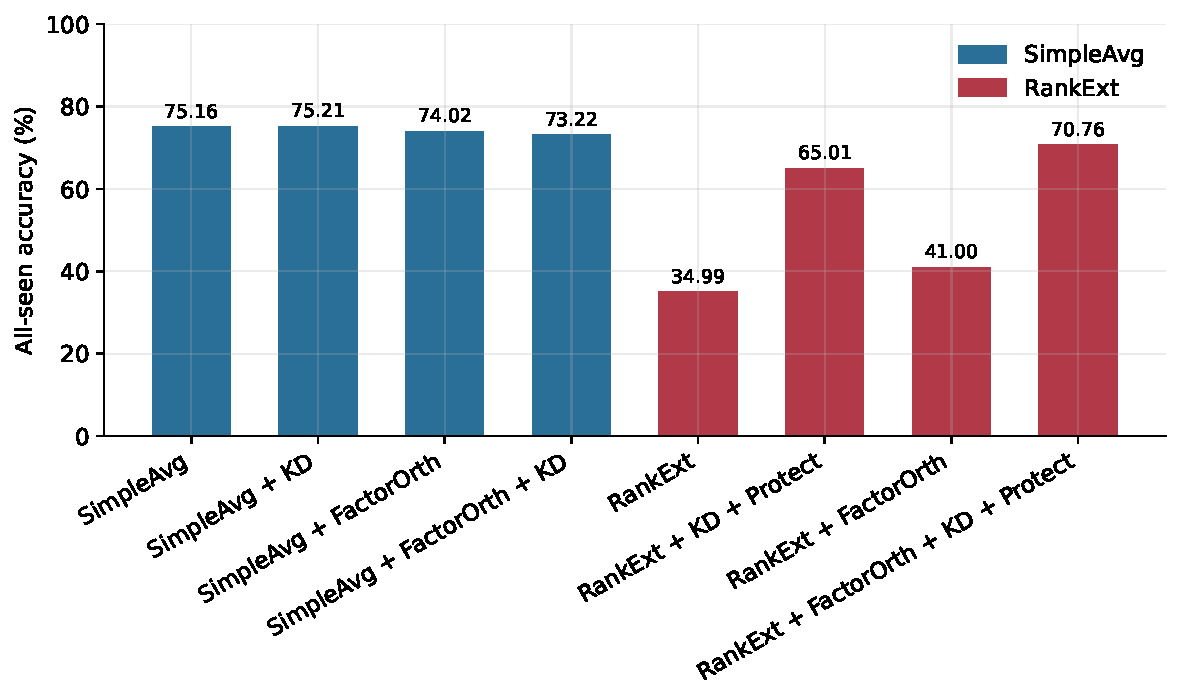
\includegraphics[width=0.95\textwidth]{figures/chapter5/cifar100_allseen_accuracy.pdf}
\caption[All-seen accuracy, main benchmark]{All-seen accuracy for the eight
canonical methods, coloured by family, zero-based axis. Source:
\texttt{chapter5\_cifar100\_8method\_main.csv}.}
\label{fig:ch5-allseen}
\end{figure}

The extended version of Table~\ref{tab:ch5-main-compact}, additionally
reporting first-task accuracy, later-tasks-mean accuracy, BWT, and
forgetting for all eight methods, is given as
Table~\ref{tab:ch5-main-extended} in Section~\ref{sec:ch5-summary}.

Two patterns are immediately visible and structure the remainder of this
chapter. The four SimpleAvg variants occupy a narrow band, from 73.22\% to
75.21\% --- a 1.99-percentage-point range. The four RankExt variants span a
much wider range, from 34.99\% to 70.76\% --- a 35.77-percentage-point
range, roughly eighteen times larger than SimpleAvg's own spread. The
highest observed SimpleAvg result in this run (SimpleAvg + KD, 75.21\%) and
the highest observed RankExt result in this run (RankExt + FactorOrth + KD +
Protect, 70.76\%) differ by \textbf{4.45 percentage points}, with SimpleAvg
ahead (Figure~\ref{fig:ch5-best-per-family}).
This single-seed gap is the cleanest one-number summary of this benchmark,
but should not be read as a significance test.

\begin{figure}[htbp]
\centering
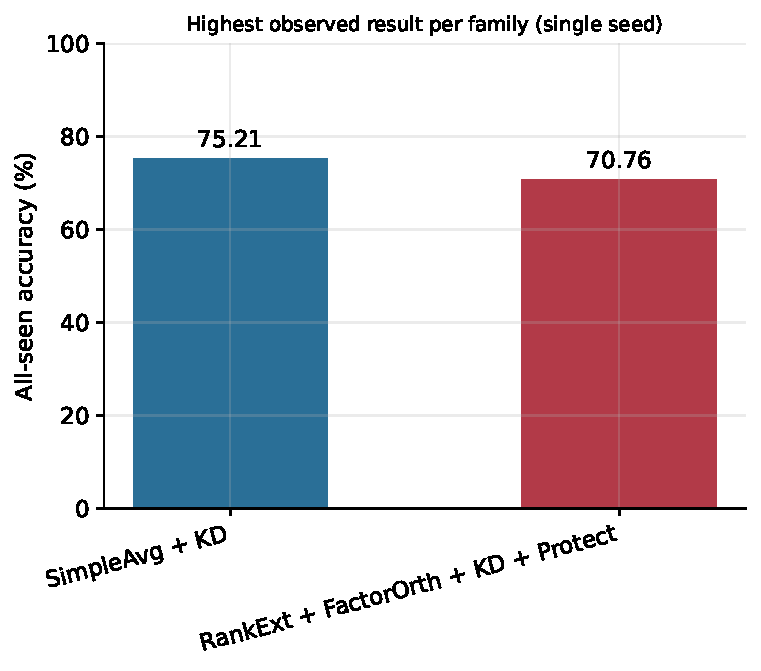
\includegraphics[width=0.55\textwidth]{figures/chapter5/cifar100_best_per_family.pdf}
\caption[Best result per family]{Best observed all-seen accuracy per family:
SimpleAvg + KD (75.21\%) versus RankExt + FactorOrth + KD + Protect
(70.76\%). A single-seed headline comparison, not a statistical significance
test.}
\label{fig:ch5-best-per-family}
\end{figure}

Read narratively: SimpleAvg establishes a strong baseline near 75\% without
requiring any auxiliary objective, and its three auxiliary-loss variants do
not move materially away from that baseline in either direction. RankExt's
plain configuration is far weaker, and the configurations with auxiliary
objectives reach substantially higher all-seen accuracy, up to 70.76\%. Sections~\ref{sec:ch5-simpleavg} and~\ref{sec:ch5-rankext}
examine each family in turn; the \emph{reasons} for this asymmetry are
deferred to Chapter~\ref{ch:discussion-conclusion}.

\section{CUB-200-2011 Cross-Dataset Evaluation}
\label{sec:ch5-cub}

The CUB-200-2011 experiment evaluates the same eight methods on a second
dataset, under the $5\times40$ protocol with seed 42
(Section~\ref{sec:ch4-datasets}). It is a supporting cross-dataset
evaluation, not a second primary benchmark: in addition to the dataset
itself, the class count, classes per step, classifier size, and
preprocessing differ from CIFAR-100, and the refined CUB-200-2011
configuration uses a RankExt classifier-head learning-rate multiplier of
$\times2$ instead of the canonical $\times1$
(Table~\ref{tab:ch4-cub-config}). Table~\ref{tab:ch5-cub-main} reports the
results.

\begin{table}[htbp]
\centering
\begin{tabularx}{\textwidth}{@{}X r r r r@{}}
\toprule
\textbf{Method} & \textbf{All-seen (\%)} & \textbf{Restricted (\%)} & \textbf{BWT} & \textbf{Forgetting} \\
\midrule
SimpleAvg & 69.47 & 91.25 & $-$0.241 & --- \\
SimpleAvg + KD & 68.69 & 91.94 & $-$0.266 & --- \\
SimpleAvg + FactorOrth & 68.33 & 91.05 & $-$0.259 & --- \\
SimpleAvg + FactorOrth + KD & 67.24 & 91.74 & $-$0.288 & --- \\
RankExt & 20.26 & 78.12 & $-$0.891 & 0.890 \\
RankExt + KD + Protect & 45.27 & 87.78 & $-$0.547 & 0.589 \\
RankExt + FactorOrth & 20.82 & 79.58 & $-$0.885 & 0.884 \\
RankExt + FactorOrth + KD + Protect & 63.43 & 88.39 & $-$0.532 & 0.570 \\
\bottomrule
\end{tabularx}
\caption[CUB-200-2011 8-method results]{CUB-200-2011 $5\times40$, seed 42:
all-seen and restricted accuracy, BWT, and forgetting for the eight methods.
BWT and forgetting follow the definitions and evaluation stages of
Section~\ref{sec:ch5-protocol}; forgetting is reported for RankExt only.
As on CIFAR-100, FactorOrth is applied to the reconstructed dense updates
for SimpleAvg ($\lambda=20$) and in the low-rank factor space for RankExt
($\lambda=50$).}
\label{tab:ch5-cub-main}
\end{table}

\textbf{SimpleAvg.} In this single-seed CUB experiment, none of the
auxiliary SimpleAvg configurations improves on the plain 69.47\% baseline:
relative to plain SimpleAvg, KD changes all-seen accuracy by $-$0.78
percentage points, FactorOrth by $-$1.14 points, and their combination by
$-$2.23 points. Restricted accuracy stays between 91.05\% and 91.94\% for
all four variants.

\textbf{RankExt.} Plain RankExt reaches 20.26\%. FactorOrth alone has only a
small observed effect ($+$0.55 percentage points, to 20.82\%). The
KD+Protect configuration, which combines knowledge distillation with the
projected feature-protection term, raises all-seen accuracy by 25.01 points
to 45.27\%, and the combined FactorOrth + KD + Protect configuration
produces the highest observed RankExt result on CUB-200-2011, 63.43\%
($+$43.17 points over plain and $+$18.16 points over KD+Protect). As on
CIFAR-100, the contributions of knowledge distillation and the projected
feature-protection term are not isolated. The highest observed SimpleAvg
result (69.47\%) and the highest observed RankExt result (63.43\%) show a
6.04-percentage-point difference in this single-seed CUB experiment.
Restricted accuracy for RankExt ranges from 78.12\% to 88.39\%, which is
lower than both the CUB-200-2011 SimpleAvg values and the CIFAR-100 RankExt
values (91.03\%--94.78\%).

\begin{table}[htbp]
\centering
\begin{tabularx}{\textwidth}{@{}X r r@{}}
\toprule
\textbf{Method} & \shortstack[r]{\textbf{CIFAR-100 $5\times20$}\\\textbf{all-seen (\%)}} & \shortstack[r]{\textbf{CUB-200-2011 $5\times40$}\\\textbf{all-seen (\%)}} \\
\midrule
SimpleAvg & 75.16 & 69.47 \\
SimpleAvg + KD & 75.21 & 68.69 \\
SimpleAvg + FactorOrth & 74.02 & 68.33 \\
SimpleAvg + FactorOrth + KD & 73.22 & 67.24 \\
RankExt & 34.99 & 20.26 \\
RankExt + KD + Protect & 65.01 & 45.27 \\
RankExt + FactorOrth & 41.00 & 20.82 \\
RankExt + FactorOrth + KD + Protect & 70.76 & 63.43 \\
\bottomrule
\end{tabularx}
\caption[CIFAR-100 versus CUB-200-2011 all-seen accuracy]{All-seen accuracy
on the CIFAR-100 primary benchmark and the CUB-200-2011 evaluation (single
seed each). This is a descriptive comparison, not a controlled estimate of
the dataset effect: the two runs also differ in class count, classes per
step, classifier size, preprocessing, and the RankExt classifier-head
learning-rate multiplier ($\times1$ on CIFAR-100, $\times2$ on
CUB-200-2011).}
\label{tab:ch5-cub-vs-cifar}
\end{table}

\textbf{Relation to CIFAR-100.} Table~\ref{tab:ch5-cub-vs-cifar} places the
two datasets side by side. The CUB experiment reproduces the main
qualitative family-level pattern observed on CIFAR-100, although the runs
are not a strict dataset-only controlled comparison because the refined CUB
configuration uses a $\times2$ RankExt classifier-head multiplier. On both
datasets, SimpleAvg is strong without auxiliary objectives and none of its
auxiliary variants clearly improves on the plain baseline; plain RankExt is
substantially weaker; FactorOrth alone does not resolve that weakness; the
KD+Protect-bearing configurations show much larger recovery; and the
combined configuration is the highest observed RankExt result without
reaching the highest observed SimpleAvg result. All-seen accuracy is
lower on CUB-200-2011 for every method, and the differences between the two
datasets are not attributed to dataset properties alone.

\section{SimpleAvg Analysis}
\label{sec:ch5-simpleavg}

Sections~\ref{sec:ch5-simpleavg}--\ref{sec:ch5-ablation} return to the
CIFAR-100 primary benchmark.

This section examines whether any of the three auxiliary mechanisms
available to SimpleAvg --- knowledge distillation (KD), FactorOrth, or their
combination --- improves on the plain arithmetic-merge baseline. For
SimpleAvg, FactorOrth is applied to the reconstructed dense updates
($\lambda=20$), whereas for RankExt it is applied directly in the low-rank
factor space ($\lambda=50$) (Section~\ref{sec:ch3-factororth}).

Table~\ref{tab:ch5-simpleavg} reports each SimpleAvg variant's delta from
plain SimpleAvg (75.16\%), alongside first-task and later-tasks-mean
accuracy.

\begin{table}[htbp]
\centering
\begin{tabularx}{\textwidth}{@{}>{\raggedright\arraybackslash}X r r r r r@{}}
\toprule
\textbf{Method} & \shortstack[r]{\textbf{All-seen}\\\textbf{(\%)}} & \shortstack[r]{\textbf{$\Delta$ vs.\ plain}\\\textbf{(pp)}} & \shortstack[r]{\textbf{First-task}\\\textbf{(\%)}} & \shortstack[r]{\textbf{Later-tasks}\\\textbf{mean (\%)}} & \shortstack[r]{\textbf{Restricted}\\\textbf{(\%)}} \\
\midrule
SimpleAvg (plain) & 75.16 & --- & 77.75 & 74.51 & 92.28 \\
SimpleAvg + KD & 75.21 & +0.05 & 68.25 & 76.95 & 92.86 \\
SimpleAvg + FactorOrth & 74.02 & $-$1.14 & 76.60 & 73.38 & 91.97 \\
SimpleAvg + FactorOrth + KD & 73.22 & $-$1.94 & 57.55 & 77.14 & 92.96 \\
\bottomrule
\end{tabularx}
\caption[SimpleAvg family results]{SimpleAvg family: all-seen accuracy,
delta from plain, first-task, later-tasks mean, and restricted accuracy.}
\label{tab:ch5-simpleavg}
\end{table}

\begin{figure}[htbp]
\centering
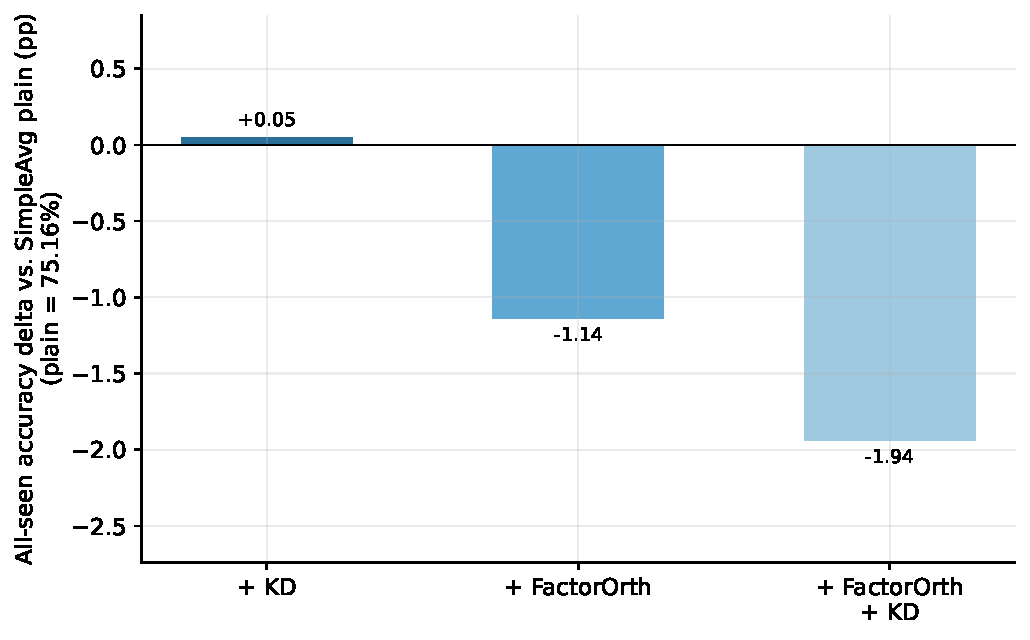
\includegraphics[width=0.75\textwidth]{figures/chapter5/cifar100_simpleavg_delta_from_plain.pdf}
\caption[SimpleAvg delta from plain]{All-seen accuracy delta of each
SimpleAvg variant relative to plain SimpleAvg, with a zero reference line.}
\label{fig:ch5-sa-delta}
\end{figure}

The +0.05 percentage-point difference between SimpleAvg + KD and plain
SimpleAvg is too small to support a meaningful improvement claim from this
single-seed experiment. Both FactorOrth
variants score below plain SimpleAvg: FactorOrth alone by 1.14 percentage
points, FactorOrth combined with KD by 1.94 percentage points, the largest
deviation from plain among the four SimpleAvg variants. None of the three
auxiliary configurations produces a clear all-seen improvement over the
plain baseline.

The near-tied all-seen numbers mask a larger redistribution across tasks.
SimpleAvg + KD's first-task accuracy (68.25\%) is 9.50 percentage points
below plain SimpleAvg's (77.75\%), while its later-tasks mean (76.95\%) is
2.44 points above plain's (74.51\%); restricted accuracy is also higher for
the KD variant (92.86\% vs.\ 92.28\%). SimpleAvg + FactorOrth + KD shows the
same direction at a larger magnitude --- first-task accuracy 57.55\% (20.20
points below plain), later-tasks mean 77.14\% (the highest later-tasks value
among the four SimpleAvg variants), restricted accuracy 92.96\% (also the
highest of the four). SimpleAvg + FactorOrth alone, without KD, does not show
this redistribution: its first-task accuracy (76.60\%) and later-tasks mean
(73.38\%) both stay close to plain's. This chapter reports the
redistribution as a factual pattern --- accuracy moves from the first task
toward later tasks whenever KD is present, roughly in proportion to how it
is combined --- without attributing a cause to it;
Chapter~\ref{ch:discussion-conclusion} addresses why.

\begin{figure}[htbp]
\centering
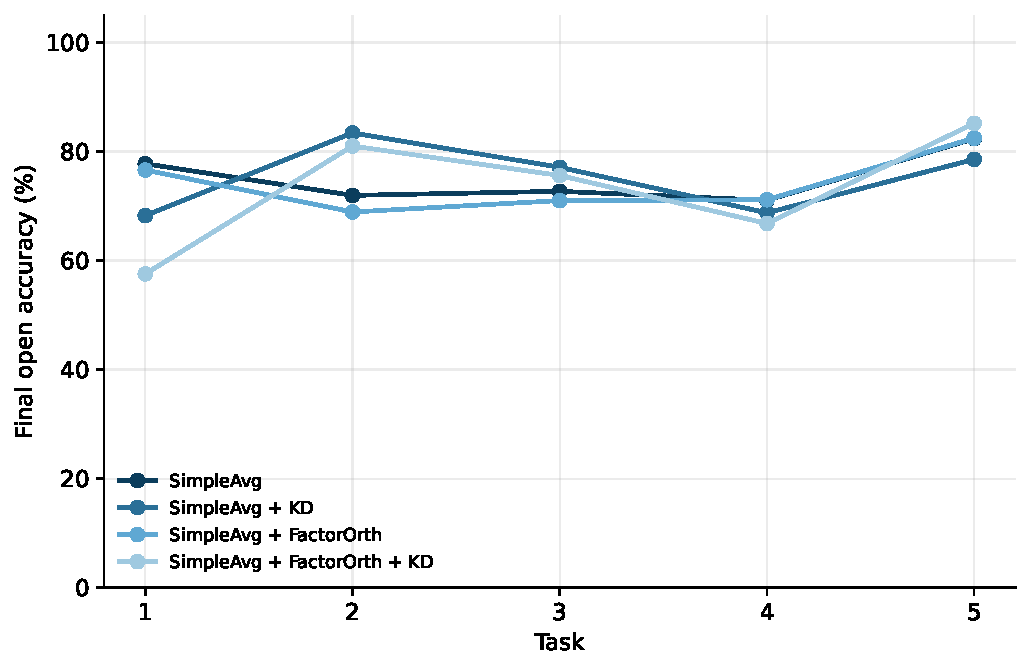
\includegraphics[width=0.75\textwidth]{figures/chapter5/cifar100_sa_per_task_final_open.pdf}
\caption[SimpleAvg per-task final open accuracy]{Final (post-sequence) open
accuracy for each of the five tasks, per SimpleAvg variant.}
\label{fig:ch5-sa-per-task-open}
\end{figure}

\begin{figure}[htbp]
\centering
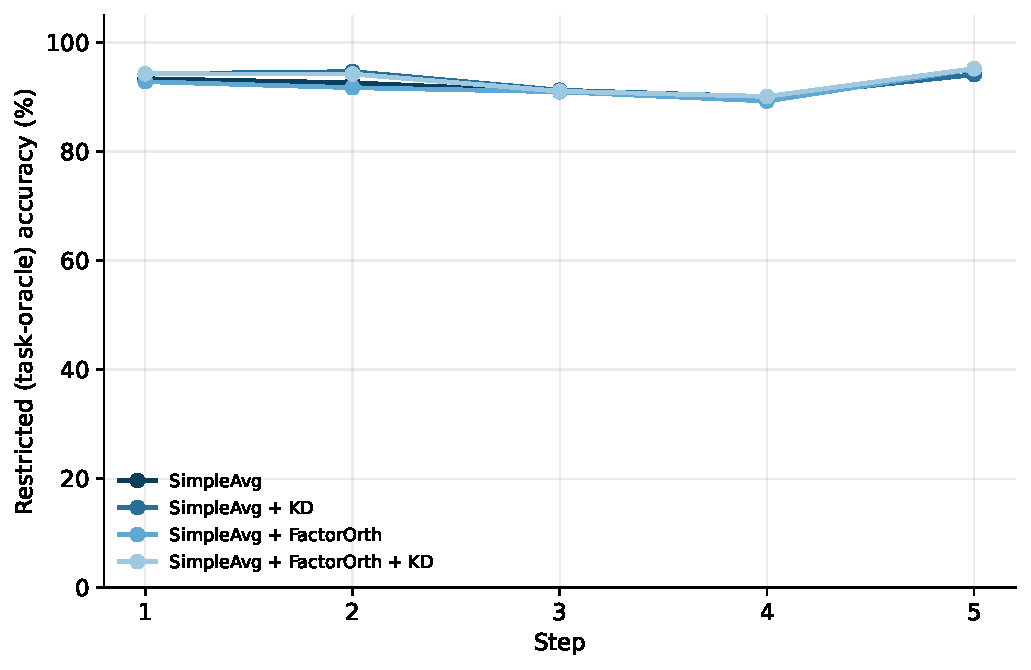
\includegraphics[width=0.75\textwidth]{figures/chapter5/cifar100_sa_per_task_restricted.pdf}
\caption[SimpleAvg per-task restricted accuracy]{Restricted (task-oracle)
accuracy for each of the five tasks, per SimpleAvg variant.}
\label{fig:ch5-sa-per-task-restricted}
\end{figure}

Per-task detail (Figures~\ref{fig:ch5-sa-per-task-open}
and~\ref{fig:ch5-sa-per-task-restricted}) shows this redistribution is not
uniform across the four non-final tasks: for both KD-bearing variants, task
1's open accuracy is the most affected, while tasks 2--4 move by smaller and
less consistent amounts. At the aggregate level, restricted accuracy
across the four SimpleAvg variants spans only 0.99 percentage points, from
91.97\% to 92.96\%. The per-task restricted results
(Figure~\ref{fig:ch5-sa-per-task-restricted}) provide the corresponding
task-level detail.

\section{RankExt Analysis}
\label{sec:ch5-rankext}

This section reports how RankExt's four variants perform relative to plain
RankExt, and presents the per-step, per-task retention trajectory underlying
the aggregate numbers.

Table~\ref{tab:ch5-rankext} reports each RankExt variant's all-seen accuracy
and its recovery over plain RankExt (34.99\%).

\begin{table}[htbp]
\centering
\begin{tabularx}{\textwidth}{@{}X r r r r r@{}}
\toprule
\textbf{Method} & \textbf{All-seen (\%)} & \textbf{$\Delta$ vs.\ plain (pp)} & \textbf{Restricted (\%)} & \textbf{BWT} & \textbf{Forgetting} \\
\midrule
RankExt (plain) & 34.99 & --- & 91.03 & $-$0.7527 & 0.8130 \\
RankExt + FactorOrth & 41.00 & +6.01 & 93.03 & $-$0.6789 & 0.7646 \\
RankExt + KD + Protect & 65.01 & +30.02 & 94.10 & $-$0.2574 & 0.3269 \\
RankExt + FactorOrth + KD + Protect & 70.76 & +35.77 & 94.78 & $-$0.1584 & 0.2474 \\
\bottomrule
\end{tabularx}
\caption[RankExt family results]{RankExt family: all-seen accuracy, delta
from plain, restricted accuracy, BWT, and forgetting.}
\label{tab:ch5-rankext}
\end{table}

\begin{figure}[htbp]
\centering
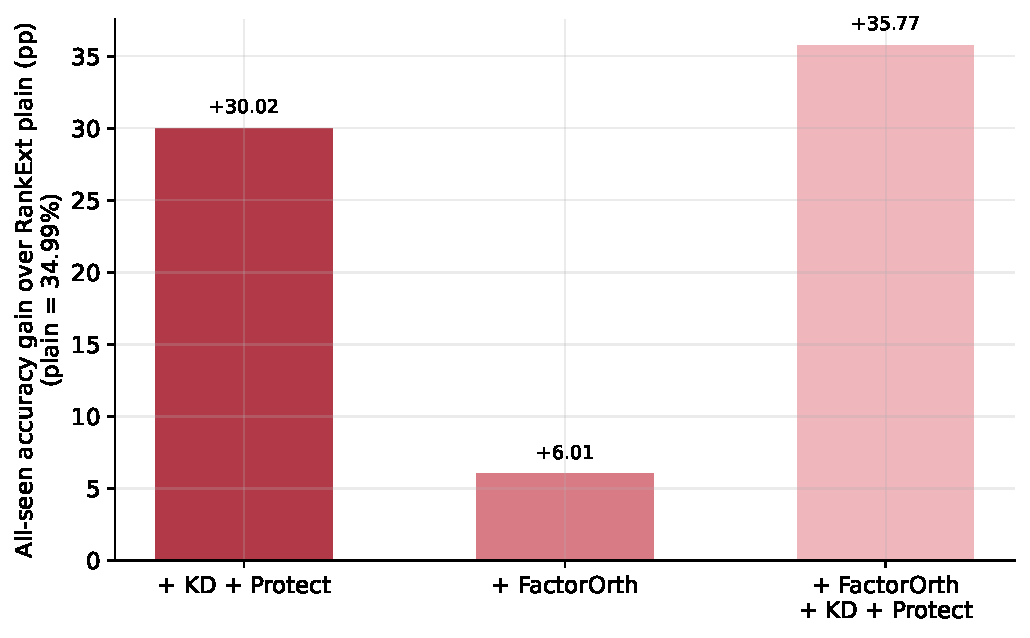
\includegraphics[width=0.75\textwidth]{figures/chapter5/cifar100_rankext_recovery_over_plain.pdf}
\caption[RankExt recovery over plain]{All-seen accuracy gain of each
enhanced RankExt variant over plain RankExt (34.99\%).}
\label{fig:ch5-rankext-recovery}
\end{figure}

Every auxiliary configuration improves on plain RankExt, and the
improvements are far from equal in size. The FactorOrth-only configuration
recovers 6.01 percentage points. The KD+Protect configuration combines
knowledge distillation with the projected feature-protection term; these
two components are not isolated from one another by a separate arm in this
benchmark. It recovers 30.02 percentage points. The combined configuration
(FactorOrth together with KD+Protect) reaches the highest observed RankExt
result in this run, 70.76\%, 35.77 percentage points above plain and 5.75
points above the KD+Protect configuration alone. BWT and forgetting improve
monotonically in the same order, consistent with the all-seen ranking. The
largest observed improvement within RankExt is therefore associated with
the KD+Protect-bearing configurations; because knowledge distillation and
projected feature protection are always active together in this benchmark,
this chapter does not attribute the improvement to either component in
isolation.

\textbf{$R_{i,j}$ trajectories.} For a sequentially-trained, persistent
model such as RankExt, this chapter additionally reports the full retention
matrix $R_{i,j}$: the open (all-seen) accuracy on task $j$, evaluated after
training has completed sequentially through task $i$ ($j \le i$). Each row
$i$ of $R_{i,j}$ is evaluated during training, immediately after task $i$
has been trained (from its best-validation checkpoint), before classifier
rescaling, with predictions taken over the full 100-way classifier output;
at $i=5$ this coincides with evaluation over all seen classes. The final
row of $R_{i,j}$ therefore describes the model before classifier rescaling,
whereas the final accuracies reported in Table~\ref{tab:ch5-main-extended}
describe the same weights after it. The two are not interchangeable: for
plain RankExt, for example, task 1 reaches 6.40\% in the final row of
$R_{i,j}$ and 11.70\% after classifier rescaling.

Figure~\ref{fig:ch5-rij-comparison} shows the four RankExt matrices together
with the SimpleAvg family, on one shared 0--100\% colour scale. Beneath
each RankExt matrix, a separate ``Final'' row gives the per-task open
accuracy of the final model after classifier rescaling. SimpleAvg does not
maintain a persistent merged model at intermediate steps, so it has no
$R_{i,j}$ trajectory; its panels show only the corresponding ``Final'' row
of the merged model, which is directly comparable to the ``Final'' rows of
the RankExt panels.

\begin{figure}[htbp]
\centering
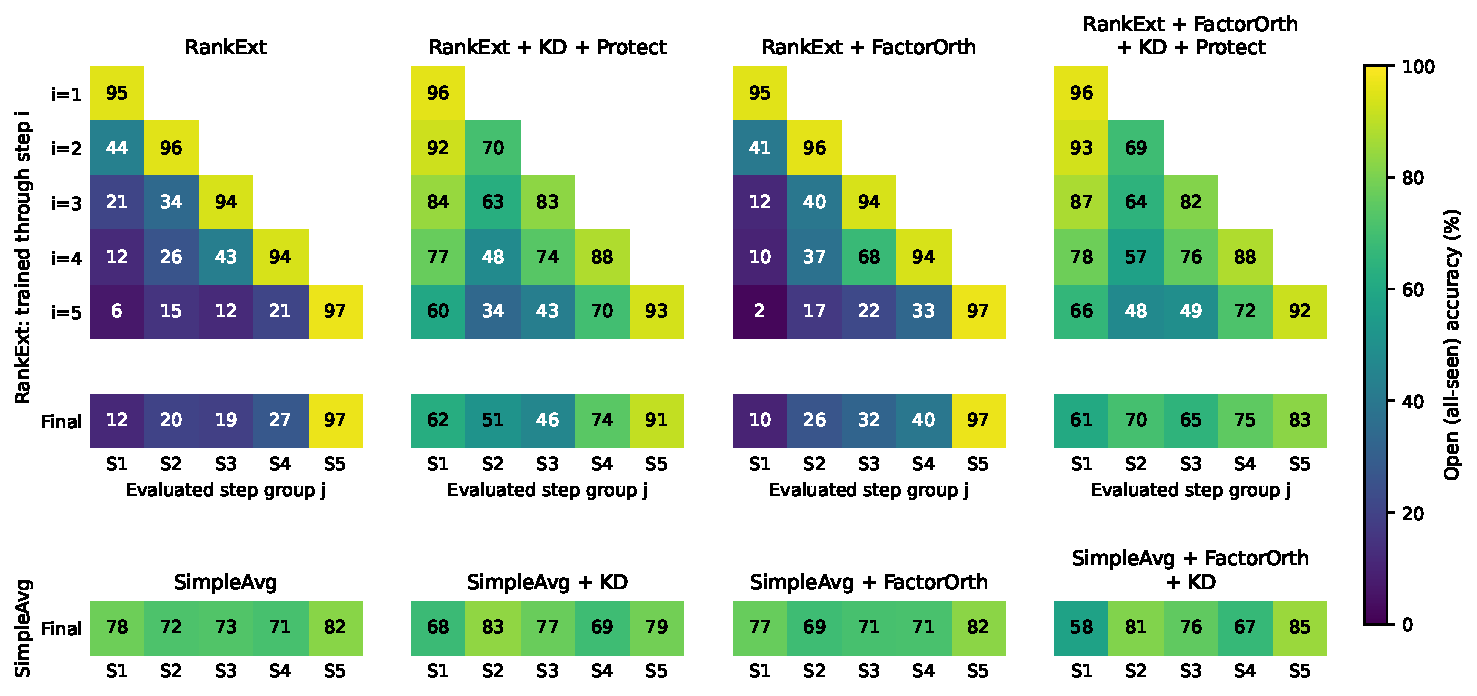
\includegraphics[width=\textwidth]{figures/chapter5/cifar100_retention_rankext_Rij_simpleavg_final.pdf}
\caption[Retention matrices and final per-task accuracy]{Open (all-seen)
accuracy per task group, shared 0--100\% colour scale. Top row: for
RankExt, the panels show the sequential $R_{i,j}$ trajectory (accuracy on
task $j$ after training through task $i$, evaluated before classifier
rescaling), followed by a separate ``Final'' row for the final model after
classifier rescaling. Bottom row: because SimpleAvg does not maintain a
persistent merged model at intermediate steps, the SimpleAvg panels report
only final merged-model per-task accuracies, after classifier rescaling.}
\label{fig:ch5-rij-comparison}
\end{figure}

Plain RankExt's matrix shows every task's own diagonal accuracy above 93\%
at the step it was learned (95.40\%, 95.70\%, 94.05\%, 93.90\%, 97.05\% for
tasks 1--5 respectively), while its off-diagonal, older-task cells decline
steeply as later tasks are trained: task 1's open accuracy, for example,
falls from 95.40\% (its own diagonal) to 43.50\% after task 2 is trained,
20.75\% after task 3, 12.10\% after task 4, and 6.40\% after task 5. The
combined configuration's matrix shows the same qualitative decline in
direction but at a markedly smaller magnitude: task 1's open accuracy after
task 5 is 66.40\%, compared with plain RankExt's 6.40\% at the same matrix
position. The KD+Protect configuration's matrix (task 1 at 60.10\% after
task 5) and the FactorOrth-only configuration's matrix (task 1 at 1.95\%
after task 5, the lowest value observed at that matrix position among the
four configurations) sit, respectively, close to and below the combined
configuration's retention level. These are reported here as factual
trajectory observations; a mechanistic account of what specifically differs
between the four configurations' retention behaviour is given in
Chapter~\ref{ch:discussion-conclusion}.

\section{Stability, Plasticity, and Open-vs-Restricted Performance}
\label{sec:ch5-stability}

This section reports the aggregate open-versus-restricted comparison across
all eight methods.

\begin{figure}[htbp]
\centering
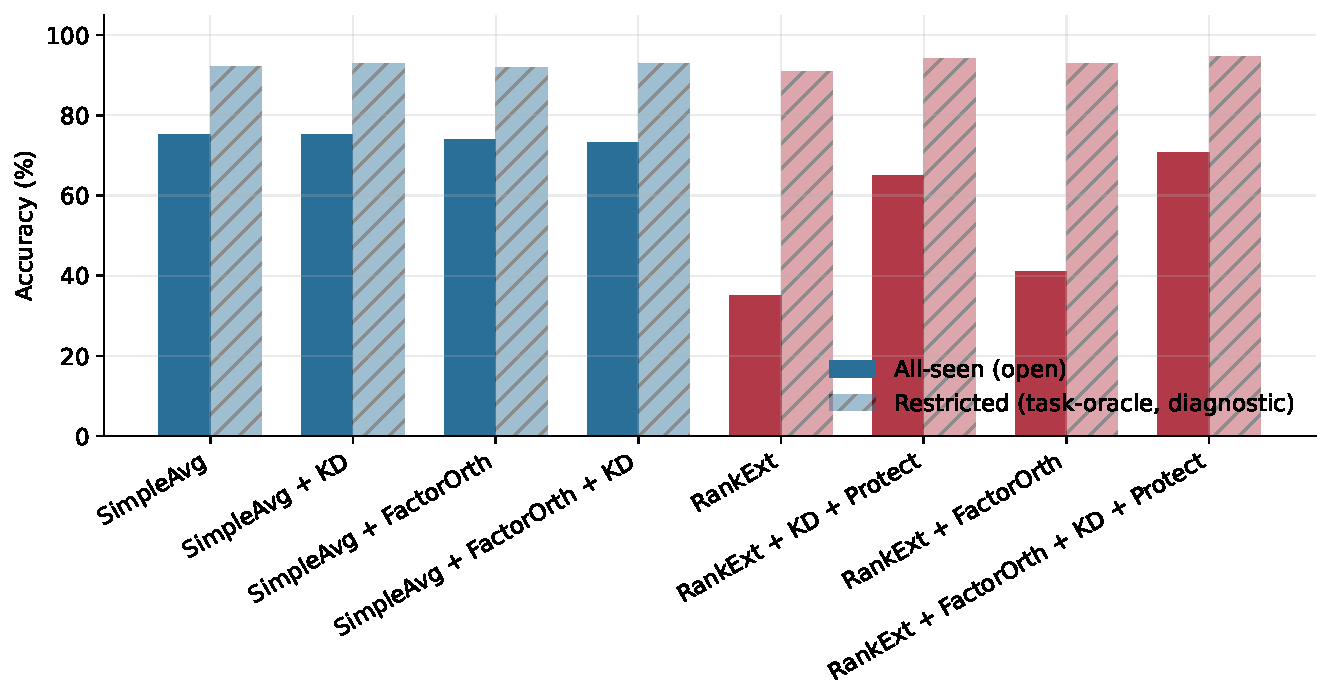
\includegraphics[width=0.85\textwidth]{figures/chapter5/cifar100_open_vs_restricted.pdf}
\caption[Open vs.\ restricted accuracy]{All-seen (open) vs.\ restricted
(task-oracle, diagnostic) accuracy for all eight methods.}
\label{fig:ch5-open-vs-restricted}
\end{figure}

Across all eight methods, restricted (task-oracle) accuracy falls in a
\textbf{91.03\%--94.78\%} range (Figure~\ref{fig:ch5-open-vs-restricted}) ---
a 3.75-percentage-point spread, far narrower than the 35.77-point spread
observed in all-seen accuracy among the four RankExt variants alone
(Section~\ref{sec:ch5-rankext}).

\begin{figure}[htbp]
\centering
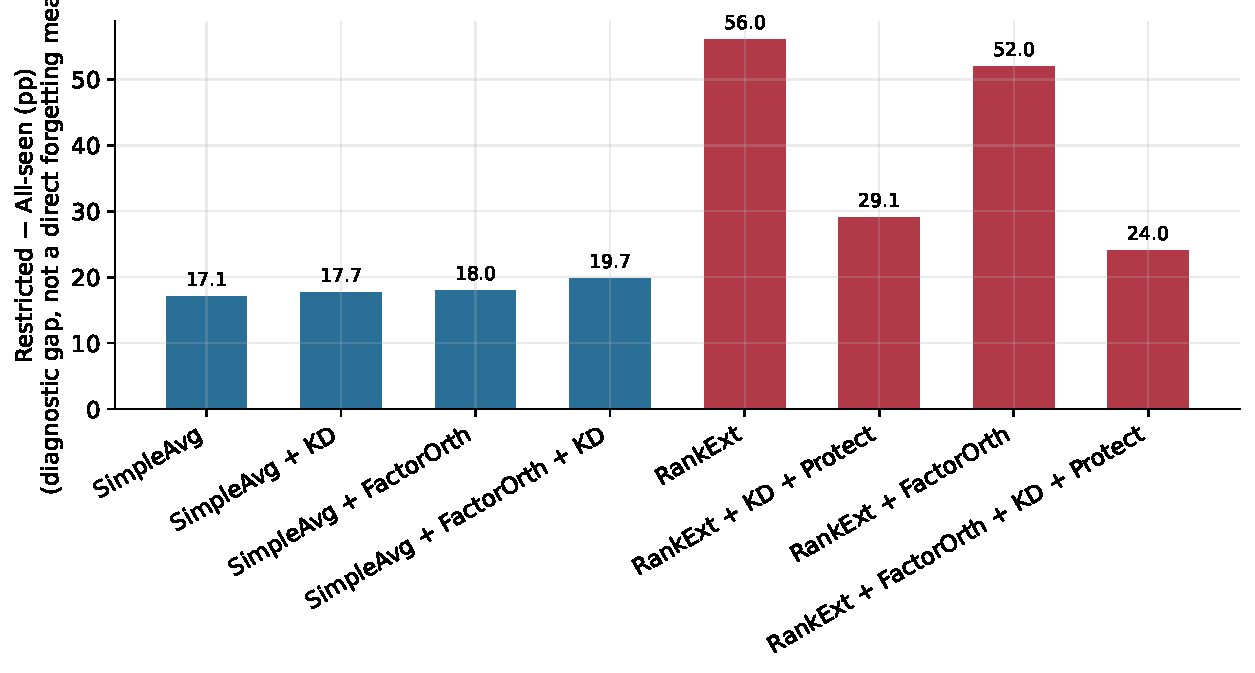
\includegraphics[width=0.85\textwidth]{figures/chapter5/cifar100_open_restricted_gap.pdf}
\caption[Open--restricted gap]{Restricted-minus-open accuracy gap per
method --- a diagnostic indicator of cross-task competition, not a direct
measure of catastrophic forgetting.}
\label{fig:ch5-open-restricted-gap}
\end{figure}

The open/restricted gap (restricted minus all-seen,
Figure~\ref{fig:ch5-open-restricted-gap}) is comparatively small and
narrow-ranging for every SimpleAvg variant (17.12 to 19.74 percentage
points, widening somewhat for the KD-bearing variants because of the
first-task redistribution described in Section~\ref{sec:ch5-simpleavg}) and
substantially larger for the two RankExt variants without KD+Protect:
plain RankExt's restricted accuracy (91.03\%) exceeds its
all-seen accuracy (34.99\%) by \textbf{56.04 percentage points}, the largest
gap of any method in this benchmark. RankExt + FactorOrth shows a comparably
large gap (93.03\% $-$ 41.00\% = 52.03 points). The two configurations that
include KD+Protect show substantially smaller gaps: RankExt + KD + Protect
(94.10\% $-$ 65.01\% = 29.09 points) and the combined configuration (94.78\%
$-$ 70.76\% = 24.02 points).

The gap indicates that within-task discrimination is substantially stronger
than task-agnostic discrimination across all seen classes, for every
RankExt configuration measured in this benchmark, and most severely for the
two configurations without KD+Protect. This is reported here as an observed
pattern. Restricted evaluation removes cross-task class competitors from the
decision rule and therefore provides a diagnostic view of within-task
discrimination; it does not identify the cause of the open-accuracy
shortfall, possible readings of which are examined in
Chapter~\ref{ch:discussion-conclusion}.

\begin{figure}[htbp]
\centering
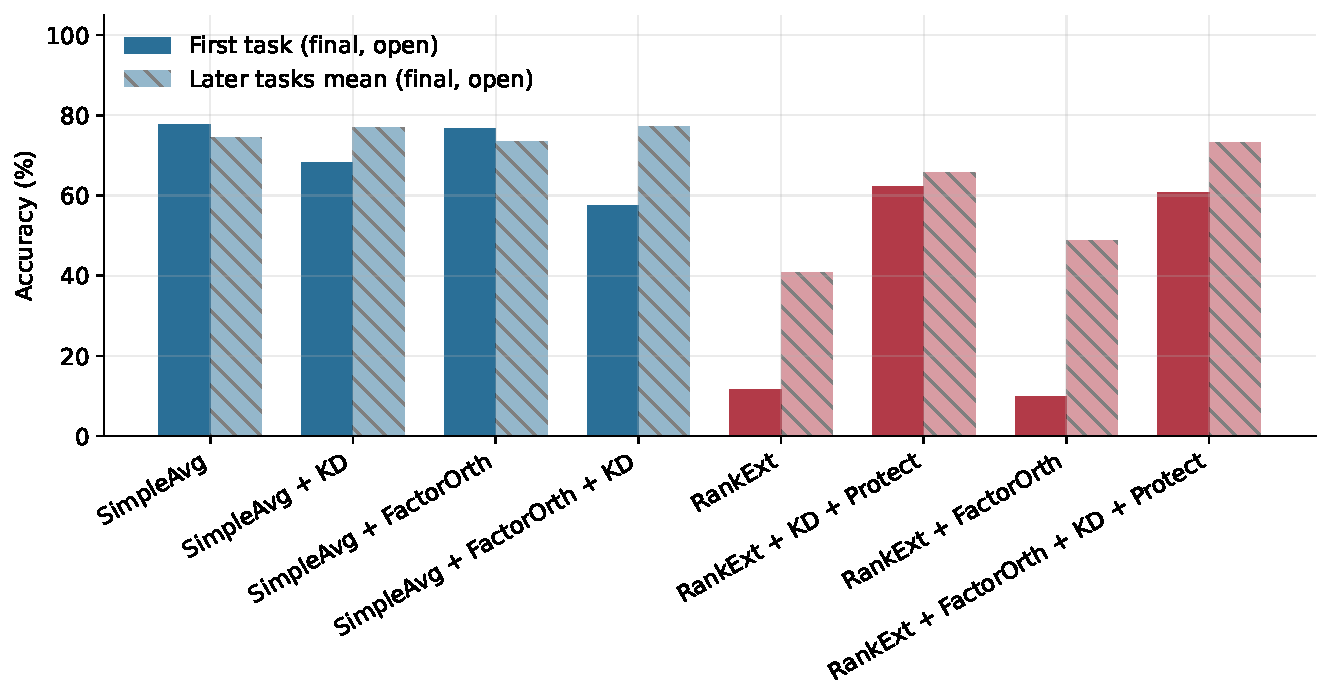
\includegraphics[width=0.85\textwidth]{figures/chapter5/cifar100_first_vs_later_tasks.pdf}
\caption[First-task vs.\ later-tasks accuracy]{First-task and later-tasks
mean accuracy for all eight methods.}
\label{fig:ch5-first-vs-later}
\end{figure}

Figure~\ref{fig:ch5-first-vs-later} presents first-task and later-tasks-mean
accuracy for all eight methods together, consolidating the per-family
patterns already reported in Sections~\ref{sec:ch5-simpleavg}
and~\ref{sec:ch5-rankext}: SimpleAvg's KD-bearing variants trade first-task
accuracy for later-tasks accuracy at roughly constant all-seen accuracy.
Within RankExt, the KD+Protect-bearing configurations substantially increase
both first-task and later-tasks accuracy relative to plain RankExt, whereas
FactorOrth alone increases later-tasks accuracy (48.79\% vs.\ 40.81\%) but
not first-task accuracy (9.85\% vs.\ 11.70\%)
(Table~\ref{tab:ch5-main-extended}).

\section{Parameter and Rank Efficiency}
\label{sec:ch5-efficiency}

This thesis is specifically concerned with LoRA-based merging and rank
extension; this section reports the structural parameter cost of each
family alongside the accuracy results of Sections~\ref{sec:ch5-main-results},
\ref{sec:ch5-simpleavg}, and~\ref{sec:ch5-rankext}, so that Chapter 5's
headline comparison is not accuracy-only.

Both families target the same 24 LoRA modules (\texttt{q\_proj} and
\texttt{v\_proj} in each of the 12 CLIP ViT-B/16 vision-encoder layers,
hidden size 768). SimpleAvg trains a fixed rank-80 adapter independently for
each of the five tasks; RankExt trains a cumulative adapter that grows by a
fixed rank-16 increment at each task, reaching a cumulative rank of 80 only
at the fifth and final task (Figure~\ref{fig:ch5-rank-growth}). The two rank
trajectories reach the same final value by construction, but represent
structurally different histories: SimpleAvg's rank-80 at every task is a
\emph{new, independent} specialist, not an accumulation; RankExt's rank-80
at task 5 is the sum of five smaller, sequentially-added, never-retrained
blocks. At the final training step, the SimpleAvg specialist rank and the
RankExt cumulative active rank are both 80; this does not imply that
SimpleAvg's final averaged dense update is itself rank-80 constrained.

\begin{figure}[htbp]
\centering
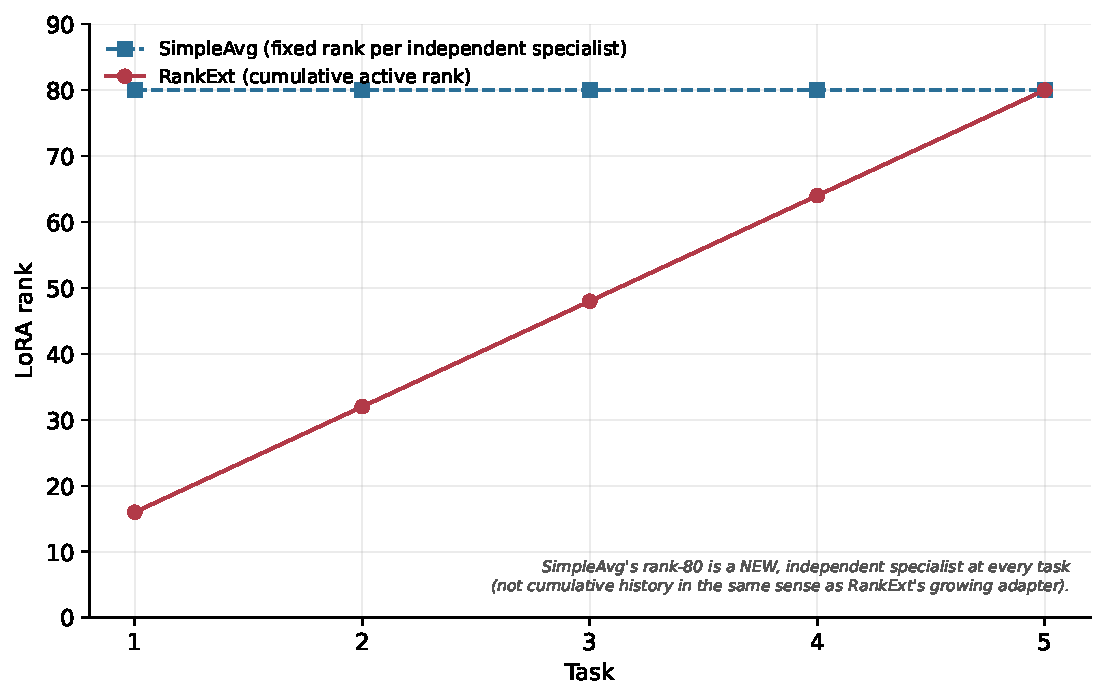
\includegraphics[width=0.8\textwidth]{figures/chapter5/cifar100_rank_growth.pdf}
\caption[LoRA rank growth]{LoRA rank used by each family across the 5-task
sequence. SimpleAvg's rank-80 is a new, independent specialist at every
task, not cumulative history in the same sense as RankExt's growing
adapter.}
\label{fig:ch5-rank-growth}
\end{figure}

Table~\ref{tab:ch5-param-efficiency} summarises the comparison.

\begin{table}[htbp]
\centering
\begin{tabularx}{\textwidth}{@{}X X X@{}}
\toprule
\textbf{Property} & \textbf{SimpleAvg} & \textbf{RankExt} \\
\midrule
Rank behaviour & Fixed rank 80, fresh independent specialist per task & Growing cumulative rank: $16{\to}32{\to}48{\to}64{\to}80$ \\
New trainable LoRA params, per task & 2{,}949{,}120 (constant) & 589{,}824 (constant) \\
LoRA parameter volume touched across all 5 tasks & 14{,}745{,}600 (5 independent adapters) & 2{,}949{,}120 (5 blocks, each trained once) \\
Final deployed LoRA overhead & 0 if the averaged delta is fused into the base model, or 14{,}155{,}776 if the dense delta is instead stored separately & 2{,}949{,}120 (kept in low-rank, additive form) \\
Final deployed classifier & 76{,}900 & 76{,}900 \\
\bottomrule
\end{tabularx}
\caption[Parameter/rank-efficiency comparison]{Structural parameter/rank
efficiency comparison, SimpleAvg vs.\ RankExt, the primary benchmark.}
\label{tab:ch5-param-efficiency}
\end{table}

\begin{figure}[htbp]
\centering
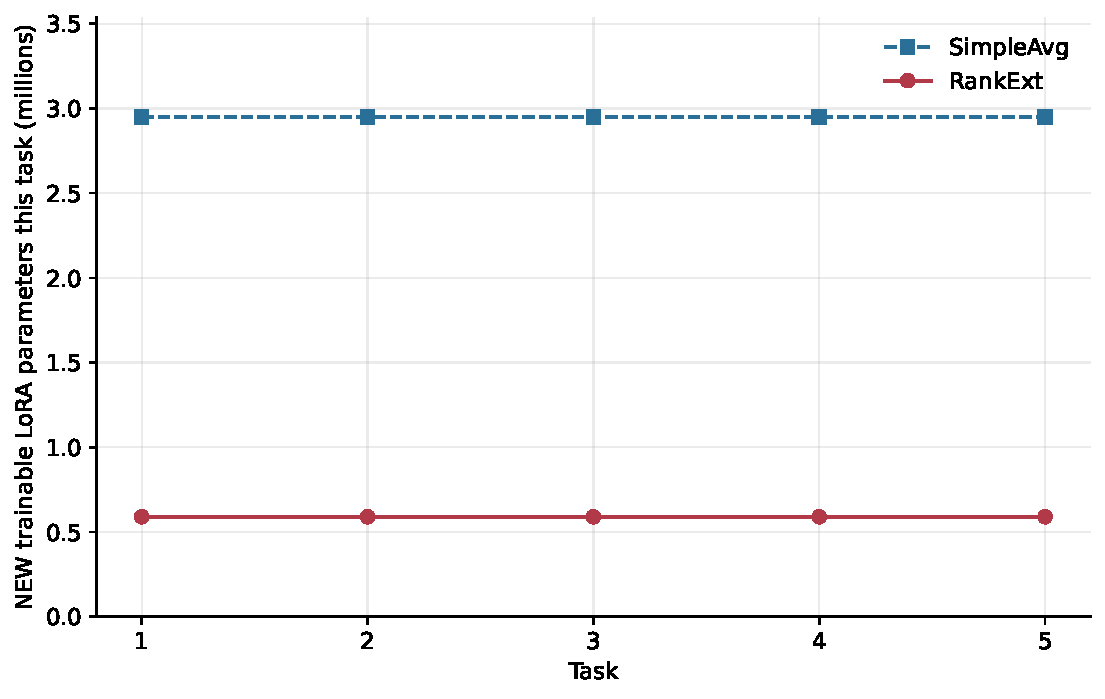
\includegraphics[width=0.8\textwidth]{figures/chapter5/cifar100_trainable_lora_params_per_task.pdf}
\caption[New trainable LoRA parameters per task]{New trainable LoRA
parameters introduced at each task, both families.}
\label{fig:ch5-trainable-params}
\end{figure}

At every task, RankExt trains fewer new parameters than SimpleAvg (589{,}824
vs.\ 2{,}949{,}120, both constant across tasks,
Figure~\ref{fig:ch5-trainable-params}). Summed across the training
sequence, RankExt's cumulative adapter reaches 2{,}949{,}120 parameters by
the final task, exactly matching its own final active rank (80), because
each of its five blocks is trained exactly once and never retrained.
SimpleAvg's five specialists, trained independently, together comprise
14{,}745{,}600 LoRA parameters over the training sequence; this is a
training-time quantity only, since the specialists are not retained
separately at deployment.

The two families also differ in \emph{how} their final adaptation is
deployed, not only in how many parameters it touches during training. In
the evaluated implementation, SimpleAvg is fused into the base weights,
whereas RankExt is retained in its low-rank additive form. SimpleAvg's merge
step averages each of its five specialists' dense
per-module weight updates and adds the averaged update directly into a copy
of the pretrained base model's own weight tensors; no separate low-rank
adapter object survives this step. If this averaged update is fused
directly into the base weights, the deployed model requires no additional
adapter parameters beyond its new 76{,}900-parameter classifier; if the
dense update is instead stored separately from an unmodified base
checkpoint (for example, for reproducibility or versioning), it occupies
14{,}155{,}776 values --- larger than the 2{,}949{,}120-parameter low-rank
form it was derived from, since the averaging step operates on dense, not
low-rank, matrices. RankExt's cumulative adapter, by contrast, is kept in
low-rank, additive form at every step, including the final one: in the
evaluated implementation its 2{,}949{,}120 parameters are not fused into the
base model's weights and remain separable from them. This chapter
reports both quantities and both deployment forms without concluding that
either family is more parameter-efficient in general; the two represent
different trade-offs between training-time parameter volume and
deployed-model structure, examined further in
Chapter~\ref{ch:discussion-conclusion}.

\section{Ablation and Refinement Results}
\label{sec:ch5-ablation}

This section reports a controlled refinement of two hyperparameters, run
separately from the primary benchmark as \textbf{the refinement experiment} and never
merged into Table~\ref{tab:ch5-main-compact} or any of the per-family tables
above. The refinement experiment changes exactly two settings relative to the primary benchmark, each
affecting one family: SimpleAvg's FactorOrth coefficient ($\lambda$) is
lowered from 20 to 1; RankExt's classifier-head learning-rate multiplier is
raised from $\times1$ to $\times2$. Every other setting is unchanged. The
two changes are family-specific and are evaluated separately against their
corresponding primary-benchmark configurations. Both comparisons below are
single-seed, controlled, two-run comparisons --- not a replication of the
primary benchmark itself.

\textbf{SimpleAvg FactorOrth, $\lambda=20$ vs.\ $\lambda=1$.}

\begin{table}[htbp]
\centering
\begin{tabularx}{\textwidth}{@{}>{\raggedright\arraybackslash}X r r r@{}}
\toprule
\textbf{Variant} & \shortstack[r]{\textbf{$\lambda=20$}\\\textbf{(the primary benchmark)}} & \shortstack[r]{\textbf{$\lambda=1$}\\\textbf{(the refinement experiment)}} & \textbf{$\Delta$ (pp)} \\
\midrule
SimpleAvg + FactorOrth & 74.02 & 73.80 & $-$0.22 \\
SimpleAvg + FactorOrth + KD & 73.22 & 74.64 & +1.42 \\
\bottomrule
\end{tabularx}
\caption[SimpleAvg FactorOrth $\lambda$ ablation]{SimpleAvg FactorOrth
(dense-update formulation) coefficient ablation, the primary benchmark ($\lambda=20$) vs.\ the refinement experiment
($\lambda=1$).}
\label{tab:ch5-sa-factororth-ablation}
\end{table}

Lowering $\lambda$ from 20 to 1 does not improve the pure FactorOrth
variant's all-seen accuracy; it is 0.22 percentage points lower at
$\lambda=1$ than at $\lambda=20$, and both values remain below plain
SimpleAvg (75.16\%, Table~\ref{tab:ch5-main-compact}). The FactorOrth+KD
variant is 1.42 points higher at $\lambda=1$ than at $\lambda=20$. Lowering
$\lambda$ therefore produced mixed effects and does not establish a superior
setting; the primary benchmark retains $\lambda=20$. This chapter reports
both deltas as observed, single-seed results; their interpretation is discussed in
Chapter~\ref{ch:discussion-conclusion}.

\textbf{RankExt classifier-head learning rate, $\times1$ vs.\ $\times2$.}

\begin{table}[htbp]
\centering
\begin{tabularx}{\textwidth}{@{}>{\raggedright\arraybackslash}X r r r@{}}
\toprule
\textbf{Variant} & \shortstack[r]{\textbf{$\times1$}\\\textbf{(the primary benchmark)}} & \shortstack[r]{\textbf{$\times2$}\\\textbf{(the refinement experiment)}} & \textbf{$\Delta$ (pp)} \\
\midrule
RankExt & 34.99 & 42.02 & +7.03 \\
RankExt + KD + Protect & 65.01 & 68.50 & +3.49 \\
RankExt + FactorOrth & 41.00 & 43.40 & +2.40 \\
RankExt + FactorOrth + KD + Protect & 70.76 & 67.92 & \textbf{$-$2.84} \\
\bottomrule
\end{tabularx}
\caption[RankExt head-LR ablation]{RankExt classifier-head learning-rate
multiplier ablation, the primary benchmark ($\times1$) vs.\ the refinement experiment ($\times2$).}
\label{tab:ch5-rankext-headlr-ablation}
\end{table}

Raising the RankExt classifier-head learning-rate multiplier from
$\times1$ to $\times2$ improves three of the four RankExt variants relative
to their primary-benchmark counterparts (+2.40 to +7.03 percentage points). The
fourth --- the combined configuration, the strongest RankExt result in the
primary benchmark (Table~\ref{tab:ch5-rankext}) --- decreases, from 70.76\%
to 67.92\%, a change of $-$2.84 percentage points. This is reported here as
an observed, single-seed result, not as evidence that the $\times2$ setting
is worse in general: the combined configuration's other metrics move in
mixed directions at $\times2$ (first-task accuracy rises from 60.70\% to
67.75\%; BWT improves from $-$0.1584 to $-$0.0532; forgetting improves from
0.2474 to 0.1289; later-tasks-mean accuracy falls from 73.28\% to 67.96\%),
a pattern reported factually here and interpreted in
Chapter~\ref{ch:discussion-conclusion}. This chapter does not claim that a
classifier-head learning-rate multiplier of $\times2$ is globally better
than $\times1$ for RankExt; the evidence is mixed across the four
configurations tested.

The $\times2$ setting was chosen after a small, reduced-scale local probe
of the combined RankExt configuration (2 tasks, 2 epochs per task, 10--15
images per class) favoured it; this probe is not benchmark evidence. Its
preference did not fully transfer to the full five-task continual
benchmark, where the strongest combined RankExt configuration regressed
(Chapter~\ref{ch:discussion-conclusion}).

\textbf{Protocol diagnostic: $4\times25$.} A separate, earlier single-seed
run (seed 42, native class order) evaluated the four RankExt configurations
under a $4\times25$ protocol: four steps of 25 classes each, covering the
same 100 classes. It uses the same RankExt implementation, full-output
knowledge distillation ($T=2$, weight 1.0), projected feature protection on
the KD-bearing configurations, factor-space FactorOrth ($\lambda=50$),
classifier-head learning-rate multiplier $\times1$, and classifier
rescaling as the primary benchmark, but differs in two further respects:
7 rather than 9 epochs per step, and a rank-20 rather than rank-16 block per
step (cumulative schedule $[20,40,60,80]$, so the final cumulative rank
remains 80). Table~\ref{tab:ch5-protocol-diag} compares final all-seen
accuracy.

\begin{table}[htbp]
\centering
\begin{tabularx}{\textwidth}{@{}X r r r@{}}
\toprule
\textbf{Method} & \shortstack[r]{\textbf{$5\times20$}\\\textbf{all-seen (\%)}} & \shortstack[r]{\textbf{$4\times25$}\\\textbf{all-seen (\%)}} & \shortstack[r]{\textbf{$\Delta$ ($4\times25-5\times20$)}\\\textbf{(pp)}} \\
\midrule
RankExt & 34.99 & 35.51 & +0.52 \\
RankExt + KD + Protect & 65.01 & 72.73 & +7.72 \\
RankExt + FactorOrth & 41.00 & 42.12 & +1.12 \\
RankExt + FactorOrth + KD + Protect & 70.76 & 73.62 & +2.86 \\
\bottomrule
\end{tabularx}
\caption[RankExt $4\times25$ protocol diagnostic]{RankExt final all-seen
accuracy under the primary $5\times20$ protocol and a secondary $4\times25$
protocol diagnostic (single seed, seed 42). The $4\times25$ run also uses
7 epochs per step and rank-20 increments ($[20,40,60,80]$); it is therefore
not a controlled single-factor comparison.}
\label{tab:ch5-protocol-diag}
\end{table}

This secondary protocol diagnostic changes the incremental partition from
five 20-class steps to four 25-class steps. It is therefore not a direct
replacement for the canonical benchmark, but provides a compact indication
of how RankExt behaves under a shallower continual sequence: all four
configurations reach a higher all-seen accuracy in this run, while plain
RankExt and FactorOrth-only RankExt remain far below the two KD+Protect
configurations.

\section{Summary and Limitations}
\label{sec:ch5-summary}

\begin{table}[htbp]
\centering
\begin{tabularx}{\textwidth}{@{}X r r r r r r@{}}
\toprule
\textbf{Method} & \textbf{All-seen} & \textbf{First-task} & \textbf{Later-tasks} & \textbf{Restricted} & \textbf{BWT} & \textbf{Forgetting} \\
\midrule
SimpleAvg & 75.16 & 77.75 & 74.51 & 92.28 & $-$0.2122 & --- \\
SimpleAvg + KD & 75.21 & 68.25 & 76.95 & 92.86 & $-$0.2001 & --- \\
SimpleAvg + FactorOrth & 74.02 & 76.60 & 73.38 & 91.97 & $-$0.2268 & --- \\
SimpleAvg + FactorOrth + KD & 73.22 & 57.55 & 77.14 & 92.96 & $-$0.2424 & --- \\
RankExt & 34.99 & 11.70 & 40.81 & 91.03 & $-$0.7527 & 0.8130 \\
RankExt + KD + Protect & 65.01 & 62.35 & 65.67 & 94.10 & $-$0.2574 & 0.3269 \\
RankExt + FactorOrth & 41.00 & 9.85 & 48.79 & 93.03 & $-$0.6789 & 0.7646 \\
RankExt + FactorOrth + KD + Protect & 70.76 & 60.70 & 73.28 & 94.78 & $-$0.1584 & 0.2474 \\
\bottomrule
\end{tabularx}
\caption[Extended main benchmark table]{Extended main-benchmark table: all
eight methods, all six metrics. All accuracy columns in percent. BWT and
forgetting are defined in Section~\ref{sec:ch5-protocol}, including the
evaluation stage (before or after classifier rescaling) of each term.}
\label{tab:ch5-main-extended}
\end{table}

\textbf{Ranking, restated concisely.} SimpleAvg's four variants cluster
within a 1.99 percentage-point band (73.22\%--75.21\%), with no auxiliary
configuration producing a clear all-seen improvement over the plain baseline
(Section~\ref{sec:ch5-simpleavg}). RankExt's four variants span a
35.77-point band (34.99\%--70.76\%); the largest observed improvement within
RankExt is associated with the KD+Protect-bearing configurations, and the
combined configuration reaches the highest observed RankExt result in this
run (70.76\%), 4.45 percentage points below the highest observed SimpleAvg
result in this run (75.21\%). RankExt's restricted accuracy remains high
(91.03\%--94.78\%) across all four configurations even where all-seen
accuracy is low, indicating that within-task discrimination is retained
more consistently than task-agnostic discrimination
(Section~\ref{sec:ch5-stability}). Parameter-efficiency accounting
(Section~\ref{sec:ch5-efficiency}) shows the two families reach comparably
sized final adapters through structurally different training and deployment
paths. A controlled refinement of two hyperparameters
(Section~\ref{sec:ch5-ablation}) improves three of the four RankExt
configurations but not the strongest one, and has mixed effects on
SimpleAvg's two FactorOrth variants. On CUB-200-2011
(Section~\ref{sec:ch5-cub}), the same qualitative family-level pattern is
observed: plain SimpleAvg (69.47\%) is not improved by any auxiliary
configuration, while RankExt rises from 20.26\% to 63.43\% with the
combined configuration.

\textbf{Limitations.} Every result presented as primary in this chapter ---
the eight-method benchmark of Section~\ref{sec:ch5-main-results}, the
per-family analyses of Sections~\ref{sec:ch5-simpleavg}--\ref{sec:ch5-efficiency},
and the refinement and protocol-diagnostic comparisons of
Section~\ref{sec:ch5-ablation} --- is a \textbf{single-seed (seed 42)}
result, and so is the CUB-200-2011 evaluation of
Section~\ref{sec:ch5-cub}. The CUB-200-2011 results add a second dataset
but do not replace repeated-seed evidence, and because the CUB-200-2011
configuration also changes the RankExt classifier-head learning rate, they
support qualitative rather than controlled cross-dataset conclusions. The reported benchmark and refinement results are single-seed
observations; no confidence intervals or statistical-significance claims
are made. Differences reported here, including the 4.45-percentage-point
SimpleAvg-vs-RankExt gap and the RankExt combined arm's $-$2.84-point change
under the head-learning-rate refinement, are this run's observed outcome.
Best-epoch selection (by validation cross-entropy, per method and per task)
means that ``final'' accuracy in this chapter is not uniformly the literal
last-epoch checkpoint for every method. The forgetting values are
reproduced exactly from the $R_{i,j}$ matrices of
Section~\ref{sec:ch5-rankext}. The BWT values are not, and the reason is
known: BWT's end-of-sequence term is measured after classifier rescaling,
whereas the final row of $R_{i,j}$ is measured before it
(Section~\ref{sec:ch5-protocol}). Substituting the post-rescaling final
accuracies for the final row of $R_{i,j}$ reproduces the reported BWT values
exactly for all four RankExt configurations; using the pre-rescaling final
row instead yields values between 0.060 and 0.089 lower.

Interpretation of the mechanisms behind these results --- why SimpleAvg's
auxiliary losses do not help, why RankExt's failure is concentrated in
open- rather than restricted-accuracy, why the head-learning-rate refinement
helps three RankExt configurations but not the fourth, and what the
parameter-efficiency and $R_{i,j}$ evidence together suggest about the two
families' underlying architectures --- is developed in
Chapter~\ref{ch:discussion-conclusion}.

\blankpage
% ============================================================================
%  Chapter 6 -- Discussion and Conclusion
%  Evidence hierarchy: (A) main benchmark; (B) controlled ablation/refinement;
%  (C) mechanistic diagnostics; (D) calibration diagnostics; (E)
%  historical/supporting runs. A lower tier is never allowed to override or
%  silently reinterpret a higher tier's result.
% ============================================================================

\chapter{Discussion and Conclusion}
\label{ch:discussion-conclusion}

\section{Main Findings}
\label{sec:ch6-main-findings}

Chapter 5's primary benchmark (CIFAR-100 $5\times20$, seed 42)
places SimpleAvg's best result (SimpleAvg + KD, 75.21\%) 4.45 percentage
points above RankExt's best result (RankExt + FactorOrth + KD + Protect,
70.76\%). Two observations drive the rest of this chapter. First,
SimpleAvg's four variants move very little around a strong plain baseline
(75.16\%): none of KD, FactorOrth, or their combination produces a clear
all-seen improvement. Second, RankExt's four variants move an order of
magnitude more (34.99\% to 70.76\%), and the movement is concentrated almost
entirely in the presence or absence of the KD+Protect configuration
($+$30.02 percentage points over plain), with FactorOrth contributing a
smaller, separate increment ($+$6.01 percentage points alone; a further
$+$5.75 points on top of KD+Protect). This chapter asks why these two
families respond so differently to auxiliary objectives that are, at the
level of Chapter~\ref{ch:methodology}'s design, addressing the same nominal
problem --- retention under sequential class-incremental training --- and
what the parameter-efficiency, $R_{i,j}$, and refinement evidence of
Chapter~\ref{ch:results} imply about that difference. Every interpretation
below is explicitly graded by the evidence tier it rests on: (A) the
primary benchmark; (B) the controlled refinement experiment;
(C) mechanistic diagnostics; (D) calibration diagnostics; (E)
historical/supporting runs. A lower tier is never allowed to override or
silently reinterpret a higher tier's result.

\section{Why SimpleAvg Is Strong}
\label{sec:ch6-simpleavg-strong}

SimpleAvg's plain baseline reaches 75.16\% without any auxiliary mechanism
(Chapter~\ref{ch:results}, Section~\ref{sec:ch5-main-results}). Several
structural properties of its design plausibly contribute to this, and this
section states them as candidate contributors, not as an isolated, proven
cause, following a dedicated evidence audit specifically constructed to
test for leakage or an unfair evaluation advantage.

That audit confirms directly from the training and evaluation code --- not
inferred --- that SimpleAvg's final evaluation is genuinely task-agnostic: a
single merged model with a single 100-way classifier head, evaluated with a
plain argmax and no task-ID routing at inference, identical in mechanism to
RankExt's own evaluation path. No leakage of task identity into final
inference was found. Given that baseline of legitimacy, several structural
properties are consistent with SimpleAvg's strength: each of its five
specialists is trained independently from a fresh pretrained checkpoint, so
no task's gradient can interfere with another task's already-learned
parameters within a single evolving model --- the sequential interference
RankExt's architecture is exposed to by construction does not arise for
SimpleAvg at all. Classifier-row stitching (Chapter~\ref{ch:methodology})
assigns each class's final row directly from the one specialist that
actually trained it, preserving an exact, task-co-adapted linear boundary
rather than blending or averaging classifier weights across tasks. This
merge-then-stitch strategy sits within the broader model-merging literature
on combining independently fine-tuned weights
\parencite{wortsman2022model,ilharco2023editing}. Fresh, full-rank-80 LoRA
specialists and a $\times10$ classifier-head learning-rate multiplier
(unchanged throughout the primary benchmark) are both consistent with,
though not individually isolated as necessary for, SimpleAvg's result.

A specific, measured capacity question is worth stating precisely rather
than left implicit. An SVD-based effective-rank measurement on real,
architecture-matched checkpoints (an earlier diagnostic run for SimpleAvg, the calibration-diagnostic checkpoint for
RankExt --- the primary benchmark's own checkpoints were unavailable locally for this
measurement, a disclosed proxy) found that SimpleAvg's merged dense delta
has 137--192 singular values exceeding 1\% of the maximum, versus 79--80
for a single specialist's own delta (roughly $1.7\times$--$2.4\times$), and
an entropy-based effective rank of 79.7--128.1 against RankExt's final
cumulative delta's 44.9--66.4 at the same sampled layers. Arithmetic
averaging of five independently-trained deltas therefore neither
destructively cancels toward the single-specialist rank ($\sim$80) nor
purely stacks toward a naive ceiling ($5\times80=400$); it lands measurably
above a single specialist's rank, in the moderate-magnitude tail of the
spectrum specifically, not concentrated in the dominant directions (stable
rank is comparable between the two families). This measurement is real and
directly relevant, but it is not, on its own, an explanation of the
4.45-percentage-point gap. Two independent controlled capacity experiments
--- a rank-32-SimpleAvg-vs-cumulative-rank-160-RankExt comparison and a
same-seed rank-80-vs-160 doubling of RankExt's own cumulative rank at fixed
SimpleAvg configuration --- both found that increasing RankExt's capacity
within the tested range closed well under 5\% of the corresponding accuracy
gap for the non-KD variants. The results are consistent with a real,
measured effective-capacity edge for SimpleAvg's merge mechanism that is
nonetheless a minor, not dominant, contributor to the observed accuracy
gap; the larger share of the gap is better explained by the mechanisms
discussed in Sections~\ref{sec:ch6-rankext-struggles}--\ref{sec:ch6-kd-protect}
below.

One further, disclosed asymmetry is worth naming without overclaiming it.
SimpleAvg's classifier head trains at a learning-rate multiplier of
$\times10$ relative to the LoRA parameters, while RankExt's (in the primary
benchmark's configuration) trains at $\times1$ --- a deliberate,
historically-documented choice (Section~\ref{sec:ch6-calibration}), not an
unexplained oversight, but one that has never been ablated back to parity
for either family. This remains an open confound on the SimpleAvg-strength
question specifically, not resolved by any evidence gathered for this
thesis.

\section{Why Knowledge Distillation Does Not Improve SimpleAvg}
\label{sec:ch6-kd-simpleavg}

Chapter~\ref{ch:results} reports that SimpleAvg + KD (75.21\%) is, at this
single seed, effectively tied with plain SimpleAvg (75.16\%, $+$0.05
percentage points), while redistributing accuracy from the first task
($-$9.50 points) toward later tasks ($+$2.44 points) and raising restricted
accuracy slightly ($+$0.58 points). This section interprets that
redistribution.

SimpleAvg's KD objective \parencite{hinton2015distilling}
(Chapter~\ref{ch:methodology}) distills only the already-introduced
(``old-seen'') classes' logits from a frozen teacher onto the student's
current-task training images, at temperature 2, with no replay of old-task
images and with current- and future-task logits excluded from the
distillation softmax entirely. This design preserves the \emph{relative}
structure among old classes as reflected on new-task images --- it
constrains how the student's old-class logits relate to one another when
evaluated on images the student is currently training on --- but it does
not directly constrain old-class predictions on old-task images themselves,
since no old-task image ever appears in this loss term, and it places no
constraint at all on the total probability mass old classes receive
relative to newly introduced classes, since the current task's own logits
are masked out of the KD softmax by construction. This is consistent with,
and offers a plausible reading of, the observed pattern: restricted
accuracy (a within-task measure, insulated from cross-task competition)
improves slightly, and later-task accuracy improves, while first-task,
all-seen-scale, open accuracy --- which depends on exactly the
old-versus-new competition this KD objective does not constrain --- does
not.

A local gradient diagnostic on the SimpleAvg+KD configuration (one training
step, two optimizer updates) provides mechanistic support, at the tier of a
diagnostic, not a benchmark result. Immediately before the first optimizer
update, the KD gradient's norm is a substantial fraction of the
cross-entropy gradient's own norm (25.48 vs.\ 33.72, a ratio of roughly
three-quarters); after one and two optimizer updates the ratio grows
slightly ($23.15/28.96 \approx 80\%$; $21.65/27.75 \approx 78\%$). The
cosine similarity between the CE and KD gradients is small and positive
before any update ($+0.053$) and becomes mildly negative after both
subsequent updates ($-0.032$, then $-0.036$). This is consistent with a
real, non-trivial optimization interaction between the two loss terms,
strong enough to materially influence the update direction, but the
gradient conflict itself is mild, not catastrophic --- a cosine near zero,
not sharply negative. Pure CE/KD gradient opposition is therefore not, on
this evidence, a sufficient explanation on its own for the
first-task-versus-later-task redistribution observed in
Chapter~\ref{ch:results}; it is one plausible contributing factor among the
scope-of-constraint argument above, and the two are consistent with each
other rather than competing explanations.

This chapter does not conclude that SimpleAvg's KD objective is broken, nor
that it should be discarded; the redistribution it produces is a real,
measured trade-off (retention on later tasks against retention on the first
task), not an unambiguous failure. It also does not conclude that post-hoc
calibration is the cause of KD's flat all-seen result --- that question is
examined on its own terms in Section~\ref{sec:ch6-calibration}.

\section{SimpleAvg FactorOrth: Optimization Strength versus Geometric Objective}
\label{sec:ch6-sa-factororth}

Although both are referred to as FactorOrth in the thesis-facing
terminology, their concrete regularisation operators differ by family:
SimpleAvg applies orthogonality to dense updates, while RankExt applies it
to normalised low-rank factors (Section~\ref{sec:ch3-factororth}). This
section concerns the SimpleAvg, dense-update formulation only; RankExt's
factor-space FactorOrth is discussed in Section~\ref{sec:ch6-factororth}.

Chapter~\ref{ch:results} reports that neither SimpleAvg + FactorOrth
(74.02\%, $-$1.14 points versus plain) nor SimpleAvg + FactorOrth + KD
(73.22\%, $-$1.94 points versus plain) improves on the plain baseline, and
that lowering SimpleAvg FactorOrth's coefficient from $\lambda=20$ (the primary benchmark) to
$\lambda=1$ (the refinement experiment, Section~\ref{sec:ch5-ablation}) does not recover
the pure SimpleAvg FactorOrth variant's accuracy (73.80\% at $\lambda=1$, still
$-$0.22 points relative to $\lambda=20$'s 74.02\%, and still below plain).
This section separates two distinct questions the SimpleAvg FactorOrth result raises:
whether $\lambda=20$ was too strong an optimization pressure, and whether
the dense-update objective itself is well-aligned with the interference it is
intended to control.

On optimization strength: an independently-computed loss-magnitude audit,
based on an earlier diagnostic run's per-arm loss logs, finds that at $\lambda=20$,
the dense-update penalty's weighted loss contribution (in that run
applied to both families) is approximately 29.1\% of the cross-entropy loss
for RankExt, but only approximately 0.04\% (alone) to
0.15\% (combined with KD) of cross-entropy for SimpleAvg --- roughly three
orders of magnitude smaller. This is a loss-magnitude ratio, not a
gradient-norm ratio, and this chapter does not conflate the two: a
separate, SimpleAvg-specific gradient-level probe measured
weighted-orthogonality-to-CE ratios directly at candidate coefficients
between 0.75 and 2.0 (not 20) and found them likewise small throughout
training (median ratios of 0.001--0.033, maximum observed ratio 0.236 at
the single largest tested coefficient and earliest measured update). No
diagnostic file located for this thesis reports a gradient-norm ratio for
the dense-update penalty at $\lambda=20$ specifically for either family; a figure of this
kind was sought and not found, and is not used in this chapter. Taken
together, the available evidence --- the loss-magnitude ratio from an
earlier diagnostic run and the refinement experiment's $\lambda=1$
ablation both moving SimpleAvg FactorOrth's pure variant
no closer to, or further from, plain SimpleAvg --- is consistent with
the dense-update penalty being numerically near-inert for SimpleAvg across the coefficient
range actually tested (1 through 20), which argues against ``$\lambda=20$
was simply too aggressive'' as the explanation for its lack of benefit: an
inert term does not become effective by being made smaller.

On the geometric objective itself: SimpleAvg FactorOrth, as implemented, penalizes
each specialist's current dense weight update against every previous
specialist's own dense update, individually and pairwise. An alternative
formulation --- orthogonality against a merged or accumulated historical
direction, or against a shared subspace spanned by all previous updates,
rather than against each individual prior update separately --- was not the
mechanism tested in either the primary benchmark or the refinement experiment. This chapter does not
claim the individual-pairwise formulation is geometrically wrong; it states
it as a plausible limitation, distinct from and additional to the
coefficient question above: even a well-tuned coefficient could leave a
geometrically-misaligned penalty unable to constrain the interference it is
meant to target. Reducing $\lambda$ addresses only the first question (was
the pressure too strong) and, on the evidence in Chapter~\ref{ch:results}'s
ablation, does not resolve the second (is the objective itself targeting
the right geometric quantity) --- the two are logically separable, and
the refinement experiment's result speaks only to the first.

\section{Why Plain RankExt Struggles}
\label{sec:ch6-rankext-struggles}

Plain RankExt reaches 34.99\% all-seen accuracy against a restricted
accuracy of 91.03\% --- a 56.04-percentage-point gap
(Chapter~\ref{ch:results}, Section~\ref{sec:ch5-stability}), the largest of
any method in the benchmark. RankExt's architecture differs from
SimpleAvg's in exactly the properties Section~\ref{sec:ch6-simpleavg-strong}
identified as plausible contributors to SimpleAvg's strength: it is a
single, persistent adapter, sequentially trained, with previously-trained
rank blocks remaining active (not retrained, but live) in every later
forward pass, and a single classifier head shared across all five tasks
from the start. This chapter reports this as the structural difference
motivating RankExt's distinct failure mode, not as itself proving what that
failure mode is mechanistically.

The Chapter~\ref{ch:results} evidence directly rules out one candidate
explanation: insufficient adaptation capacity.
Section~\ref{sec:ch6-simpleavg-strong} already reports that two independent
controlled capacity experiments --- doubling RankExt's cumulative rank at
fixed protocol, and a rank32-SimpleAvg-vs-rank160-RankExt comparison in
which RankExt has substantially more nominal capacity than SimpleAvg ---
both find that increased capacity closes well under 5\% of the
corresponding gap for RankExt's non-KD variants, and in the plain case can
leave accuracy essentially unchanged or slightly worse. Within the tested
capacity range, capacity alone does not explain plain RankExt's weakness.
The open/restricted divergence itself
(Section~\ref{sec:ch6-open-restricted}) is more directly diagnostic:
restricted accuracy --- a within-task measure, insulated from competition
against other tasks' logits --- remains high (91.03\%) even as open,
all-seen accuracy collapses, which is inconsistent with a simple loss of
discriminative features and more consistent with a cross-task, output-space
competition effect, examined further below and in
Section~\ref{sec:ch6-open-restricted}. A companion audit of candidate
mechanisms found one further mechanism directly measured, on a related
variant set (not identical to the primary benchmark's own arms):
representation/feature drift, via a
cosine-alignment diagnostic comparing an old task's features to its own
classifier row versus the most recently trained row, strongly implicates
feature drift for non-KD RankExt configurations specifically. The primary benchmark's
non-KD arms (plain and FactorOrth-only) already include a training-time
mitigation for this --- a pretrained-feature anchor loss --- adopted in
response to that earlier diagnosis, meaning their reported
34.99\%/41.00\% results are already post-mitigation, not pre-fix numbers.

\section{The Role of KD+Protect in RankExt's Recovery}
\label{sec:ch6-kd-protect}

RankExt + KD + Protect reaches 65.01\% ($+$30.02 percentage points over
plain), the majority of the total recovery achieved by the combined
configuration (70.76\%). Following Chapter~\ref{ch:results}'s own
convention, this chapter attributes this recovery to the KD+Protect
configuration as a whole: full-scope, 100-way knowledge distillation and
the classifier-row feature-protection term are both active in every
RankExt arm that includes either, and this thesis's evidence does not
isolate their individual contributions from one another. This chapter does
not state that knowledge distillation alone causes this recovery.

Two properties of this configuration are consistent with why it addresses
RankExt's failure mode more directly than FactorOrth alone
(Section~\ref{sec:ch6-factororth}). Full-scope KD's teacher softmax spans
every class introduced so far, including the classes the student is
currently learning, so the distillation loss directly constrains the
\emph{relative scale} between old and newly introduced classes' logits ---
precisely the axis Section~\ref{sec:ch6-rankext-struggles}'s open/restricted
evidence implicates as the dominant failure mode, and precisely the
constraint SimpleAvg's differently-scoped, old-seen-only KD objective
(Section~\ref{sec:ch6-kd-simpleavg}) does not provide. The projected
feature-protection term penalizes the student's feature displacement, for
old classes, against a subspace derived from those classes' own classifier
rows --- a targeted retention constraint distinct in mechanism from KD's
output-space constraint. Both readings are offered as plausible
mechanistic accounts consistent with the measured result, not as
individually isolated causal findings; no ablation in this thesis separates
KD's contribution from Protect's.

\section{RankExt FactorOrth and KD+Protect}
\label{sec:ch6-factororth}

FactorOrth alone recovers 41.00\% from plain RankExt's 34.99\% ($+$6.01
percentage points) --- a real but much smaller recovery than KD+Protect's
$+$30.02 points. Combined with KD+Protect, the full recipe reaches 70.76\%,
a further $+$5.75 points above KD+Protect alone
(Chapter~\ref{ch:results}, Section~\ref{sec:ch5-rankext}). One plausible
interaction is that FactorOrth's weight-geometry regularization ---
penalizing the current rank block's factor-space cosine similarity against
previous blocks --- controls a different aspect of the adapter's structure
than KD+Protect's output-space and feature-space constraints, and that its
benefit is correspondingly larger when paired with a mechanism that already
addresses old-task retention directly. This is stated as an interaction
consistent with the measured pattern, not as a statistically established
synergy: this thesis ran no seed replication of any RankExt arm, and the
ablation evidence in Section~\ref{sec:ch6-calibration} shows this
interaction's sign is not stable across configurations (the
head-learning-rate refinement reverses it, Section~\ref{sec:ch6-calibration}).
FactorOrth alone, without KD+Protect, is not sufficient to close a
meaningful share of RankExt's gap to SimpleAvg --- its own-arm result
(41.00\%) remains far below SimpleAvg's weakest variant (73.22\%).

\section{Stability--Plasticity Trade-off}
\label{sec:ch6-stability-plasticity}

Chapter~\ref{ch:results}'s first-task, later-tasks-mean, BWT, and forgetting
values, its $R_{i,j}$ trajectories, and the head-learning-rate refinement's
combined-arm result together describe a consistent stability--plasticity
pattern \parencite{kirkpatrick2017overcoming,delange2022continual}:
mechanisms that improve retention of earlier tasks can reduce a model's
accuracy on tasks introduced later, and the balance is sensitive to exactly
how strongly a retention mechanism is applied, not only to whether one is
present. SimpleAvg's KD-bearing variants trade first-task accuracy for
later-task accuracy at roughly unchanged all-seen accuracy
(Section~\ref{sec:ch6-kd-simpleavg}). RankExt's auxiliary configurations
raise both first-task and later-task accuracy relative to plain, in an
order that matches their overall all-seen ranking --- auxiliary mechanisms
here improve both axes simultaneously, rather than trading one for the
other, which is a materially different pattern from SimpleAvg's.

The clearest single instance of this trade-off in this thesis is the
RankExt head-learning-rate refinement (the refinement experiment,
Section~\ref{sec:ch5-ablation}): raising the classifier-head learning-rate
multiplier from $\times1$ to $\times2$ improves three of the four RankExt
configurations, but the combined configuration --- the strongest result in
the primary benchmark --- regresses, from 70.76\% to 67.92\% ($-$2.84
percentage points). This regression is not a uniform degradation:
first-task accuracy improves ($60.70\% \to 67.75\%$, $+$7.05 points), BWT
improves ($-0.1584 \to -0.0532$), and forgetting improves ($0.2474 \to
0.1289$), while later-tasks-mean accuracy falls ($73.28\% \to 67.96\%$).
This is consistent with, and directly illustrates, the stability--plasticity
trade-off this section describes: at $\times2$, the combined configuration
becomes more stable on earlier tasks and less plastic on later ones, at
this single seed, and the net all-seen effect of that shift is negative for
this specific, most heavily retention-constrained configuration, even
though the same directional shift is net-positive for the three
configurations with fewer or weaker retention constraints. This chapter
interprets this as evidence that the optimal degree of classifier-head
plasticity for RankExt is not independent of which retention mechanisms
are simultaneously active in a given configuration --- raising plasticity
helps a lightly-constrained arm and can hurt a heavily-constrained one ---
rather than as evidence that either learning-rate setting is globally
preferable.

\section{The Local Head-Learning-Rate Probe and the Full Production Run}
\label{sec:ch6-lr-probe}

This section corrects an important point of scope that is easy to state
imprecisely. The local decision probe that informed the refinement experiment's choice of
a $\times2$ classifier-head learning-rate multiplier for RankExt tested the
\textbf{same RankExt method} used in the primary benchmark's flagship arm
--- the full FactorOrth + KD + Protect combined configuration --- not a
simpler or differently-composed RankExt variant. The final-compare script
that extended the sweep to LR$=1.0$ and LR$=2.0$ is confirmed, by direct
comparison, to be a byte-for-byte copy of the decision-probe script,
differing only in the swept learning-rate values, their assertions, and the
run-name prefix; both scripts target this one method exclusively. What
differs between the probe and the primary/ablation production runs is
\textbf{scale}, not \textbf{method}: the probe trained on 2 tasks (not 5),
2 epochs per task (not 9), and 10--15 images per class (not the full
dataset). Within that reduced scale, the probe found validation
cross-entropy and every measured accuracy metric improving monotonically as
the learning-rate multiplier increased across $\{0.1, 0.2, 0.5\}$ and then
across $\{0.5, 1.0, 2.0\}$, consistently across two seeds, with no
exception on any headline metric.

The full 5-task, 9-epoch, full-dataset production run (the refinement experiment) does not
reproduce this finding for the one configuration the probe actually tested:
the combined arm's accuracy falls under $\times2$
(Section~\ref{sec:ch6-stability-plasticity}). Three of the four RankExt
configurations --- none of which were the probe's own tested configuration
--- do improve under $\times2$, consistent with the probe's directional
finding extended by analogy, not by direct test, to those other
configurations. This is best read as a genuine methodological lesson about
probe scale, not about probe scope: a small-scale decision probe, run on
the exact production method it was meant to inform, correctly identified
the direction of the effect within the range it tested, but did not --- and
at that scale could not have been expected to --- predict that the same
method's response to a longer, full-length continual sequence, with five
tasks' worth of accumulated retention constraints active simultaneously
rather than two, would reverse sign for that specific,
already-most-heavily-constrained configuration. This chapter treats the
probe's own within-scale conclusion as sound and treats the discrepancy as
evidence that short, few-task decision probes may not extrapolate reliably
to longer continual sequences for a configuration that is already close to
its own stability--plasticity limit, rather than as evidence the probe
itself was flawed in design or target.

\section{Open versus Restricted Performance and Cross-Task Competition}
\label{sec:ch6-open-restricted}

The open/restricted divergence is the most consistent pattern across every
RankExt configuration in Chapter~\ref{ch:results}
(Section~\ref{sec:ch5-stability}): restricted accuracy stays in a narrow
91.03\%--94.78\% band across all eight methods in the benchmark, while
all-seen accuracy for RankExt alone spans 34.99\% to 70.76\%. Plain
RankExt's own gap (56.04 percentage points) is the largest observed. This
indicates, as Chapter~\ref{ch:results} states factually, that within-task
class discrimination remains substantially stronger than task-agnostic
discrimination for the affected configurations --- restricted accuracy, by
construction, measures whether the correct class is still favored once
competition from other tasks' classes is removed, and that measurement
stays high even where the full, unrestricted competition collapses the
same model's accuracy.

Multiple, not mutually exclusive, mechanisms are consistent with this
pattern, and this chapter does not conclude the gap is purely a calibration
artifact, nor that it demonstrates zero forgetting. Cross-task logit
competition --- newer tasks' logits systematically out-competing older
tasks' logits in the shared argmax --- is consistent with the monotone,
step-by-step decline visible in the $R_{i,j}$ matrices
(Chapter~\ref{ch:results}, Section~\ref{sec:ch5-rankext}): each old task's
open accuracy erodes as more tasks are trained, while its own diagonal
(just-learned) accuracy and its restricted accuracy both stay high
throughout. Score-scale mismatch between task groups is directly, though
diagnostically, evidenced by the post-hoc calibration result discussed in
Section~\ref{sec:ch6-calibration}. Representation drift is separately
implicated, for non-KD RankExt configurations specifically, by the
cosine-alignment diagnostic cited in
Section~\ref{sec:ch6-rankext-struggles}. These mechanisms plausibly coexist
rather than compete: a model can simultaneously retain within-task
discriminative structure, suffer some genuine representation drift for
non-KD-protected old tasks, and have its surviving structure obscured at
the output-space level by inter-task score misalignment. This thesis's
evidence does not decompose the 56.04-percentage-point plain-RankExt gap,
or any other configuration's smaller gap, into precise shares attributable
to each mechanism.

\section{Calibration as Diagnostic Headroom}
\label{sec:ch6-calibration}

A separate, explicitly diagnostic line of evidence bears on the
score-scale-mismatch reading above. A post-hoc, validation-fitted
inter-task logit-scale calibration \parencite{zhao2020maintaining} --- one
positive multiplicative scalar per task group, four free parameters, fit by
minimizing validation cross-entropy with no backbone, LoRA, or classifier
retraining and no test-set tuning --- was evaluated against an earlier,
separately-trained RankExt combined-arm checkpoint (6 epochs, no Protect30
term, not the primary benchmark's own weights, which were unavailable
locally for this diagnostic). On that checkpoint: raw, uncalibrated open
accuracy was
34.67\%; the pipeline's own historical row-norm calibration alone reached
53.12\% (matching that run's own reported result); adding the
four-parameter scale calibration reached 70.74\%, a further $+$17.62
percentage points, while restricted accuracy remained exactly unchanged at
93.68\% before and after (proven exactly invariant by construction, not
merely observed to be similar) --- direct evidence that a substantial
share of that specific checkpoint's residual open/restricted gap is
attributable to a correctable inter-task logit-scale mismatch, not to
further loss of within-task discriminative structure. The fitted scales
(2.147, 1.224, 1.178, 0.932, with the most recent task fixed at 1.0 as
reference) decrease roughly monotonically from oldest to most recent task,
consistent with a recency-competition reading: older tasks' logits needed
the largest upward correction to compete fairly against newer tasks'.

This chapter uses the term \textbf{post-hoc, validation-fitted inter-task
logit-scale calibration} throughout, and avoids ``classifier-weight
correction'' or ``corrected average weights'': the mechanism never touches
stored classifier weights, LoRA factors, or the merged dense delta; it
rescales the already-computed logit vector at inference time only, via a
small, separate module distinct from the model's own parameters. It is also
worth stating precisely what ``task-aware'' means here: the four scale
parameters are fit using knowledge of the fixed 20-class task-group
boundaries, but no per-sample task identity is required or used at
inference --- every test image is scored by the same, already-fitted,
group-wise rescaled classifier, regardless of which task it belongs to. The
mechanism is therefore task-structure-aware at calibration time and
task-agnostic at per-example inference time.

This result is reported strictly as diagnostic headroom, not as main
benchmark evidence, and for three compounding reasons: it was measured on
that earlier checkpoint, not the primary benchmark's own; that earlier
run lacks the Protect30 term and uses a different epoch count from the
primary benchmark, so its own 53.12\% starting point is not directly
comparable to the primary benchmark's 70.76\%; and the coincidence that
70.74\% (this diagnostic, on a weaker
starting checkpoint) lands close to the primary benchmark's own combined-arm result
(70.76\%, achieved through a different mechanism --- full-scope KD,
Protect30, and the pipeline's own more sophisticated row-norm calibration)
is noted as a striking but uncontrolled observation, not evidence that the
two mechanisms are interchangeable or additive. A related run, the calibration-diagnostic experiment,
applies this style of calibration (though not identically parameterized) to
RankExt while simultaneously changing SimpleAvg's classifier-head learning
rate; because the two changes are confounded within that run, the calibration-diagnostic experiment is
used in this chapter only as a second, independent diagnostic data point,
never as benchmark evidence: relative to the primary benchmark, it shows large gains
for RankExt configurations without a prior bias-correction mechanism
($+$32.71 and $+$31.47 percentage points for plain and FactorOrth-only
respectively) and small or negative changes for configurations that
already include KD+Protect ($+$1.75 and $-$1.17 percentage points for
KD+Protect and the combined configuration respectively) --- a pattern
consistent with calibration and KD+Protect addressing overlapping headroom
in the same underlying inter-task competition problem, though the calibration-diagnostic experiment's
own confound (the simultaneous SimpleAvg regression) prevents this from
being stated as a clean, isolated finding.

\section{Parameter and Rank Efficiency}
\label{sec:ch6-efficiency}

Chapter~\ref{ch:results}'s parameter-efficiency accounting
(Section~\ref{sec:ch5-efficiency}) shows the two families reach the same
final adapter size (a rank-80-equivalent, 2{,}949{,}120 LoRA parameters)
through structurally different training and deployment paths, and this
chapter does not conclude either is more efficient in general --- the two
represent different trade-offs, separable into training cost, storage, and
deployment overhead, each considered in turn.

\textbf{Training cost.} SimpleAvg trains 2{,}949{,}120 new LoRA parameters
at every one of its five tasks (a fresh, full rank-80 specialist each
time), for a cumulative training-time volume of 14{,}745{,}600 parameters
across the sequence. RankExt trains only 589{,}824 new parameters at each
task (a single new rank-16 block, with all earlier blocks frozen and never
retrained), for a cumulative training-time volume of 2{,}949{,}120 ---
exactly RankExt's own final adapter size, because each of its five blocks
is trained exactly once. RankExt is therefore substantially cheaper in
training-time parameter volume at every stage of the sequence, a genuine
structural property of its incremental design, independent of the accuracy
results discussed above.

\textbf{Deployment form.} The two families do not merely differ in size at
deployment; they differ in kind. SimpleAvg's merge step averages its five
specialists' dense per-module weight updates and adds the averaged update
directly into the pretrained base model's own weight tensors --- no
separate, low-rank adapter object survives this step. If the averaged
update is fused directly into the base weights, as the training pipeline
does, the deployed model requires no additional adapter parameters beyond
its 76{,}900-parameter classifier; the underlying rank-80-equivalent
structure that produced that update is not present in the deployed model
as a distinct, removable component. If, instead, the dense update were
stored separately from an unmodified base checkpoint --- for
reproducibility, versioning, or to keep a shared base model usable by
multiple downstream adapters --- it would occupy 14{,}155{,}776 values,
larger than the 2{,}949{,}120-parameter low-rank form it was derived from,
because the averaging step itself operates in dense, not factored, weight
space. This chapter does not treat the dense-storage figure as SimpleAvg's
default or mandatory deployment representation; it is one possible
representation, quantified because the fused, in-place form (SimpleAvg's
actual default) has no separately-quantifiable ``extra parameter'' figure
at all. RankExt's cumulative adapter, in contrast, remains in low-rank,
additive form at every step through deployment: its 2{,}949{,}120
parameters sit alongside an unmodified base model, addable and removable as
a distinct object, never fused into the base weights.

RankExt's structural advantage is therefore progressive, low training-time
cost and a persistent, separable adapter structure --- not, on this
evidence, a smaller final adapter than SimpleAvg's, since the two reach the
same nominal rank-80-equivalent size. SimpleAvg's structural advantage is a
final deployment representation that, once fused, requires no separate
adapter bookkeeping at all, at the cost of five times the training-time
parameter volume to reach it and no accessible low-rank structure at any
intermediate point in the sequence (a property directly connected to
Section~\ref{sec:ch5-rankext}'s observation that SimpleAvg has no genuine
$R_{i,j}$ trajectory: without a persistent, evolving intermediate model,
there is nothing to evaluate at ``after training through task $i$,
$i<5$''). No wall-clock or FLOPs measurement was made for either family in
this thesis; the comparison above is a parameter-count and
deployment-structure comparison only, and this chapter does not extend it
to computational cost.

\section{Limitations}
\label{sec:ch6-limitations}

The most consequential limitation is that every result presented as
primary in this thesis --- the primary benchmark, the ablation/refinement
comparison, and every number in this chapter drawn from either --- is a
\textbf{single-seed (seed 42)}
production result. No repeated-seed evidence exists for the primary
benchmark; the 4.45-percentage-point SimpleAvg-versus-RankExt gap, the
RankExt combined arm's $-$2.84-point response to the head-learning-rate
refinement, and every mechanistic interpretation offered above rest on this
single run each. A canonical multi-seed replication plan for the primary
benchmark exists but had not been executed at the time of writing.

Several of this chapter's auxiliary mechanisms are bundled, not
individually isolated: KD and Protect30 are never tested apart from one
another in RankExt (Section~\ref{sec:ch6-kd-protect}); FactorOrth's
interaction with KD+Protect is observed, not statistically isolated
(Section~\ref{sec:ch6-factororth}); the SimpleAvg FactorOrth loss-magnitude finding
and the SimpleAvg FactorOrth gradient-level probe come from different runs at
different coefficients, not a single controlled sweep through $\lambda=20$
itself. SimpleAvg's calibration behavior (a small-sample diagnostic: plain
accuracy moving from 84\% to 83\% with calibration on versus off, and the
KD variant moving from 83\% to 75\%, both on a 100-image evaluation subset)
is a real but tiny-sample observation that has not been run at benchmark
scale, and may confound comparisons between SimpleAvg configurations if
calibration interacts differently with each. BWT is constructed differently
for the two families by necessity (Section~\ref{sec:ch5-protocol}) and the
two families' BWT values, though tabulated together for compactness, are
not structurally comparable. SimpleAvg has no standard, persistent
$R_{i,j}$ trajectory to evaluate, for the structural reason given in
Section~\ref{sec:ch6-efficiency}, not a logging gap. The local
head-learning-rate probes and gradient/effective-rank diagnostics cited
throughout this chapter are, by their own design and by this thesis's own
evidence hierarchy, diagnostic only --- informative about direction and
mechanism, never substituted for benchmark evidence. A second dataset,
needed to test whether any conclusion in this chapter is specific to
CIFAR-100's particular class structure, had not been evaluated at the time
of writing. Finally, this thesis's parameter-efficiency comparison
(Section~\ref{sec:ch6-efficiency}) covers parameter counts and deployment
structure only; no wall-clock training time or FLOPs measurement was made
for either family, and no claim in this chapter should be read as a
computational-cost comparison.

\section{Future Work}
\label{sec:ch6-future-work}

The evidence gathered in this thesis motivates several specific,
evidence-grounded directions, stated in priority order rather than as a
generic list.

\textbf{Reformulate SimpleAvg FactorOrth's geometric target.}
Section~\ref{sec:ch6-sa-factororth}'s distinction between optimization strength
and geometric alignment motivates testing an orthogonality penalty against
a merged or accumulated historical direction, or against a subspace
spanned by all previous updates jointly, rather than against each
individual prior specialist's update pairwise --- a test that would
isolate whether the dense-update formulation, not only its coefficient, limits
its usefulness.

\textbf{Disentangle KD from Protect30 in RankExt.} No arm in this thesis
tests full-scope KD without the projected feature-protection term, or
Protect30 without KD, for RankExt; Section~\ref{sec:ch6-kd-protect}'s
attribution to ``the KD+Protect configuration'' as a whole is the most
precise claim this evidence supports, and resolving it further requires
this specific ablation.

\textbf{Revisit KD's data distribution for SimpleAvg, including
replay-aware variants.} Section~\ref{sec:ch6-kd-simpleavg}'s
scope-of-constraint argument suggests that a KD objective exposed to
old-task images directly (rather than only old-class logits on new-task
images), or an explicitly replay-aware distillation design, would more
directly constrain the axis Chapter~\ref{ch:results}'s evidence identifies
as unaddressed by the current old-seen, no-replay formulation.

\textbf{Complete calibration-aware continual learning as an integrated, not
diagnostic-only, mechanism.} Section~\ref{sec:ch6-calibration}'s headroom
result, measured only on a non-primary checkpoint, is a strong-tier
diagnostic finding but a weak-tier claim about the primary benchmark
specifically; the natural next step is fitting and evaluating the same
calibration mechanism against the primary benchmark's own checkpoints directly, and,
if it holds, integrating it as part of the trained or
immediately-post-training pipeline rather than a separate diagnostic pass.

\textbf{Multi-seed replication of the primary benchmark and the
head-learning-rate refinement.} Section~\ref{sec:ch6-limitations}'s
single-seed limitation applies to every quantitative claim in this thesis;
the combined-arm regression under the head-learning-rate refinement
(Sections~\ref{sec:ch6-stability-plasticity}--\ref{sec:ch6-lr-probe}) is
the single most novel and most seed-fragile finding, and is the
highest-priority candidate for replication.

\textbf{A second dataset}, to test whether the SimpleAvg-versus-RankExt
structural account developed in this chapter is a property of the two
architectures generally or is in some way specific to CIFAR-100's class
structure --- ImageNet-100 is a natural candidate; no results for a second
dataset exist at the time of writing.

\textbf{Protocol depth.} Every result in this thesis uses the primary
$5\times20$ protocol. Whether RankExt's behaviour, and its position
relative to SimpleAvg, changes when the same 100 classes are partitioned
into fewer or more incremental steps, with the total class count and final
cumulative rank held fixed (Section~\ref{sec:protocol-depth}), is not
examined here and is a natural controlled extension of this work.

\textbf{A retention-schedule or plasticity-aware learning-rate policy for
RankExt}, motivated directly by
Section~\ref{sec:ch6-stability-plasticity}'s finding that a single fixed
classifier-head learning rate does not suit every RankExt configuration
equally --- a schedule sensitive to how many retention mechanisms are
simultaneously active, rather than a single global multiplier, is a
plausible, evidence-motivated next step.

\textbf{Feature-space preservation as a complementary retention mechanism
for RankExt}, distinct from both KD's output-space constraint and
FactorOrth's weight-geometry constraint, is a plausible additional lever
suggested by, but not tested in, this thesis's mechanistic diagnostics
(Section~\ref{sec:ch6-rankext-struggles}'s representation-drift finding for
non-KD arms).

\section{Final Conclusion}
\label{sec:ch6-conclusion}

Within the evaluated setting --- CIFAR-100, $5\times20$ class-incremental
protocol, seed 42 --- this thesis's central empirical finding is an
asymmetry between two structurally different approaches to continual LoRA
adaptation. SimpleAvg, an architecturally simple strategy of independently
training per-task specialists and merging them once at the end, is
unexpectedly strong: it reaches 75.16\% without any auxiliary retention
mechanism, and none of the auxiliary mechanisms tested in this thesis ---
knowledge distillation, an orthogonality penalty, or their combination ---
improves on that baseline in any way this thesis can distinguish from
single-seed noise. RankExt, a persistent, incrementally-growing adapter
architecture, requires explicit retention mechanisms to approach
SimpleAvg's result at all: plain RankExt reaches only 34.99\%, and the
combination of full-scope knowledge distillation, classifier-row feature
protection, and a weight-geometry orthogonality penalty recovers most,
though not all, of the resulting gap, reaching 70.76\% --- 4.45 percentage
points below SimpleAvg's best result.

The evidence in this chapter is consistent with this asymmetry being
substantially structural rather than a matter of tuning either family
further within the settings already tested. RankExt's single, persistent,
shared classifier head exposes it to a cross-task, output-space
competition effect that its restricted-accuracy evidence shows is not
primarily a loss of underlying discriminative features; SimpleAvg's
independent-specialist, classifier-stitching design largely avoids this
competition by construction, at the cost of substantially higher
training-time parameter volume and a final deployment form that discards
its low-rank structure entirely. Auxiliary constraints that directly
target RankExt's output-space competition --- full-scope KD and
classifier-row protection --- recover the large majority of its deficit;
auxiliary constraints layered onto SimpleAvg's already-effective
architecture do not find an equivalent defect to repair, and in
the case of SimpleAvg FactorOrth appear numerically inert at every coefficient tested.
Cross-task score alignment remains a major, only partially resolved,
residual issue for RankExt: post-hoc calibration evidence, diagnostic and
not yet confirmed on the primary benchmark's own checkpoints, suggests a
substantial further share of its remaining gap is a correctable
scale-mismatch problem rather than additional representation damage.

More generally, this thesis's parameter-efficiency and
stability--plasticity evidence together indicate that parameter-efficient
continual adaptation via LoRA involves a genuine trade-off, not a single
dominant strategy, between independent-specialist merging and persistent,
incremental growth: the former is inexpensive to deploy but expensive to
train and architecturally blind to any notion of sequential state; the
latter is inexpensive to train incrementally and retains an inspectable,
persistent structure, but is exposed to cross-task interference that must
be actively managed, and the correct degree of that management is itself
sensitive to which other mechanisms are simultaneously active, as the
head-learning-rate refinement's mixed result demonstrates directly. This
thesis does not identify a universal winner between the two strategies
beyond the settings evaluated here; it identifies, with evidence at
multiple tiers, \emph{why} the two strategies fare differently under these
settings, and what would be required --- multi-seed replication, a second
dataset, and several specific, targeted follow-up experiments named in
Section~\ref{sec:ch6-future-work} --- to extend these conclusions further.

\blankpage

% \backmatter is redefined by DEIthesis.cls: it prints the bibliography, then
% the acknowledgments (frontmatter/thanks.tex), then switches to \appendix.
\backmatter

\chapter{Appendix 1}
\label{app:appendix1}
\section{Hyperparameter and Protocol Reference}
\label{sec:appA-hyperparameters}

Table~\ref{tab:appA-hyperparams} consolidates, in one place, the exact
per-family configuration used for the primary benchmark
(Chapter~\ref{ch:results}). Every value here is already established in
Chapter~\ref{ch:experimental-setup} or Chapter~\ref{ch:results}; it is
repeated here as a single quick-reference table rather than as new
information.

\begin{table}[htbp]
\centering
\begin{tabularx}{\textwidth}{@{}X X X@{}}
\toprule
\textbf{Setting} & \textbf{SimpleAvg} & \textbf{RankExt} \\
\midrule
Backbone & \multicolumn{2}{l}{CLIP ViT-B/16 vision encoder (frozen), hidden size 768} \\
LoRA target modules & \multicolumn{2}{l}{\texttt{q\_proj}, \texttt{v\_proj}, all 12 layers (24 modules)} \\
LoRA rank & 80 (fixed, per specialist) & Cumulative: $16{\to}32{\to}48{\to}64{\to}80$ \\
LoRA alpha & 160 & $2\times$ cumulative rank at each step \\
Classifier-head LR multiplier & $\times10$ & $\times1$ \\
FactorOrth formulation & Dense-update orthogonality & Factor-space orthogonality \\
FactorOrth $\lambda$ & $\lambda=20$ (1-epoch warmup) & $\lambda=50$ (1-epoch warmup) \\
KD scope & Old-seen only, no replay & Full (100-way) \\
KD temperature & 2 & 2 \\
KD warmup & 1 epoch & None \\
Projected feature-protection term & --- & Weight 30, KD-bearing RankExt arms only \\
Epochs per step & \multicolumn{2}{l}{Maximum 9 (plain SimpleAvg: early stopping, 5--8)} \\
Optimizer / scheduler & \multicolumn{2}{l}{AdamW, cosine schedule, 10\% warmup ratio} \\
Replay & \multicolumn{2}{l}{None (rehearsal-free)} \\
Classifier rescaling & \multicolumn{2}{l}{Confidence-weighted, regime-grouped row-norm rescaling} \\
Seed & \multicolumn{2}{l}{42} \\
\bottomrule
\end{tabularx}
\caption[Hyperparameter reference]{Consolidated hyperparameter and protocol
reference for the primary CIFAR-100 benchmark.}
\label{tab:appA-hyperparams}
\end{table}

Table~\ref{tab:appA-datasets} lists the settings that differ between the
CIFAR-100 primary benchmark and the CUB-200-2011 evaluation
(Section~\ref{sec:ch4-datasets}); every setting not listed there is shared.

\begin{table}[htbp]
\centering
\begin{tabularx}{\textwidth}{@{}l X X@{}}
\toprule
\textbf{Setting} & \textbf{CIFAR-100} & \textbf{CUB-200-2011} \\
\midrule
Classes & 100 & 200 \\
Protocol & $5\times20$ (primary; $4\times25$ secondary diagnostic) & $5\times40$ \\
Class order & Native label order & Fixed seed-42 permutation \\
Classifier & $768\to100$ & $768\to200$ \\
SimpleAvg rank & 80 & 80 \\
RankExt schedule & $16{\to}32{\to}48{\to}64{\to}80$ & $16{\to}32{\to}48{\to}64{\to}80$ \\
SimpleAvg head-LR multiplier & $\times10$ & $\times10$ \\
RankExt head-LR multiplier & $\times1$ & $\times2$ \\
Projected feature-protection term & Weight 30 (KD-bearing RankExt arms) & Weight 30 (KD-bearing RankExt arms) \\
Validation & 25 images per class, from the training set & 5 images per class, from the official training split \\
Evaluation split & CIFAR-100 test set & Official CUB-200-2011 test split \\
Preprocessing & As in Table~\ref{tab:ch4-training-config} & Aspect-ratio-preserving CLIP resize; deterministic centre-crop evaluation \\
Seed & 42 & 42 \\
\bottomrule
\end{tabularx}
\caption[Dataset-specific settings]{Dataset-specific settings of the
CIFAR-100 primary benchmark and the CUB-200-2011 evaluation.}
\label{tab:appA-datasets}
\end{table}

\section{Local Head-Learning-Rate Decision Probe}
\label{sec:appA-lr-probe}

Table~\ref{tab:appA-lr-probe} reports the reduced-scale local decision
probe discussed in Section~\ref{sec:ch6-lr-probe}, which tested the
combined RankExt configuration (FactorOrth + full KD + projected feature
protection) at
2 steps, 2 epochs per step, and 10--15 images per class, across two seeds
(42 and 123). These figures are explicitly non-benchmark, reduced-scale
diagnostic evidence, reported here in full only because
Section~\ref{sec:ch6-lr-probe} refers to them by summary; they are never
compared numerically against any Chapter~\ref{ch:results} benchmark value.

\begin{table}[htbp]
\centering
\begin{tabularx}{\textwidth}{@{}X X X X@{}}
\toprule
\textbf{Head-LR multiplier} & \textbf{Validation CE (mean $\pm$ std)} & \textbf{All-seen accuracy (mean $\pm$ std)} & \textbf{Restricted mean accuracy} \\
\midrule
$\times0.5$ & $3.9055 \pm 0.0033$ & $16.00\% \pm 2.12$ & $25.00\%$ \\
$\times1.0$ & $3.6389 \pm 0.0120$ & $21.75\% \pm 1.77$ & $32.75\%$ \\
$\times2.0$ & $3.1455 \pm 0.0168$ & $36.50\% \pm 4.24$ & $52.00\%$ \\
\bottomrule
\end{tabularx}
\caption[Local head-LR decision probe]{Local, reduced-scale head-LR
decision probe on the combined RankExt configuration (2 seeds; 2 steps, 2
epochs/step, 10--15 images/class). Non-benchmark diagnostic evidence.}
\label{tab:appA-lr-probe}
\end{table}

\section{RankExt $R_{i,j}$ Retention Matrices, Full Numeric Values}
\label{sec:appA-rij}

Tables~\ref{tab:appA-rij-plain}--\ref{tab:appA-rij-combined} give the exact
open (all-seen) accuracy values underlying the four RankExt $R_{i,j}$
trajectories shown in the top row of Figure~\ref{fig:ch5-rij-comparison},
for readers who want precise numbers rather than a colour scale. These are
in-training evaluations made before classifier rescaling. The ``Final''
rows of that figure, and its SimpleAvg panels, correspond to the final
per-step accuracies after classifier rescaling; SimpleAvg has no
intermediate merged model and therefore no $R_{i,j}$ table. $R_{i,j}$ is the accuracy on step $j$ after
training has completed through step $i$ ($j \le i$); empty cells are
structurally undefined (a step cannot be evaluated before it is trained).

\begin{table}[htbp]
\centering
\begin{tabular}{@{}l ccccc@{}}
\toprule
 & T1 & T2 & T3 & T4 & T5 \\
\midrule
After step 1 & 95.40 & & & & \\
After step 2 & 43.50 & 95.70 & & & \\
After step 3 & 20.75 & 34.00 & 94.05 & & \\
After step 4 & 12.10 & 26.05 & 42.65 & 93.90 & \\
After step 5 & 6.40 & 14.90 & 11.80 & 20.75 & 97.05 \\
\bottomrule
\end{tabular}
\caption[$R_{i,j}$ matrix -- RankExt plain]{RankExt (plain), open accuracy
(\%), $R_{i,j}$.}
\label{tab:appA-rij-plain}
\end{table}

\begin{table}[htbp]
\centering
\begin{tabular}{@{}l ccccc@{}}
\toprule
 & T1 & T2 & T3 & T4 & T5 \\
\midrule
After step 1 & 95.40 & & & & \\
After step 2 & 40.55 & 96.05 & & & \\
After step 3 & 11.65 & 39.55 & 93.95 & & \\
After step 4 & 10.05 & 37.15 & 67.85 & 94.10 & \\
After step 5 & 1.95 & 16.55 & 21.90 & 33.25 & 97.05 \\
\bottomrule
\end{tabular}
\caption[$R_{i,j}$ matrix -- RankExt + FactorOrth]{RankExt + FactorOrth,
open accuracy (\%), $R_{i,j}$.}
\label{tab:appA-rij-factororth}
\end{table}

\begin{table}[htbp]
\centering
\begin{tabular}{@{}l ccccc@{}}
\toprule
 & T1 & T2 & T3 & T4 & T5 \\
\midrule
After step 1 & 95.75 & & & & \\
After step 2 & 92.40 & 70.35 & & & \\
After step 3 & 84.45 & 62.75 & 82.85 & & \\
After step 4 & 76.60 & 47.85 & 73.90 & 88.25 & \\
After step 5 & 60.10 & 33.70 & 42.90 & 69.75 & 93.45 \\
\bottomrule
\end{tabular}
\caption[$R_{i,j}$ matrix -- RankExt + KD + Protect]{RankExt + KD +
Protect, open accuracy (\%), $R_{i,j}$.}
\label{tab:appA-rij-kdprotect}
\end{table}

\begin{table}[htbp]
\centering
\begin{tabular}{@{}l ccccc@{}}
\toprule
 & T1 & T2 & T3 & T4 & T5 \\
\midrule
After step 1 & 95.75 & & & & \\
After step 2 & 93.15 & 69.10 & & & \\
After step 3 & 87.40 & 64.50 & 81.60 & & \\
After step 4 & 77.75 & 57.10 & 76.10 & 88.05 & \\
After step 5 & 66.40 & 47.60 & 49.45 & 72.10 & 92.05 \\
\bottomrule
\end{tabular}
\caption[$R_{i,j}$ matrix -- RankExt combined]{RankExt + FactorOrth + KD +
Protect (combined), open accuracy (\%), $R_{i,j}$.}
\label{tab:appA-rij-combined}
\end{table}


\chapter{Core Implementation Listings}
\label{app:code}
% ============================================================================
%  Appendix B -- Core Implementation Listings
% ----------------------------------------------------------------------------
%  The two listings are presentation copies kept in code/. Their executable
%  statements were checked (AST comparison, comments/docstrings ignored)
%  against the canonical production script used for the primary CIFAR-100
%  run; only comments, docstrings, and whitespace differ.
% ============================================================================

\lstdefinestyle{appendixListing}{
  style=codeSnippet,
  language=Python,
  basicstyle=\ttfamily\footnotesize,
  numberstyle=\scriptsize\color{numColor},
  numbers=left,
  numbersep=6pt,
  xleftmargin=2.2em,
  framexleftmargin=2.2em,
  breaklines=true,
  breakatwhitespace=true,
  postbreak=\mbox{\ensuremath{\hookrightarrow}\space},
  showstringspaces=false,
  columns=fullflexible,
  keepspaces=true,
  upquote=true
}

The listings in this appendix reproduce the core implementation logic
underlying the two integration strategies compared in this thesis. Only the
integration-specific code is shown; data loading, training loops, logging,
plotting, diagnostics, and experiment orchestration are omitted. The
executable logic is extracted from the production implementation used for
the primary experiment; comments and docstrings have been lightly cleaned
for readability, and some long statements re-wrapped.

\section{SimpleAvg Dense-Update Merge}
\label{sec:appB-simpleavg}

SimpleAvg trains one independent LoRA specialist per incremental step, each
starting from the pretrained backbone. At the end of every step,
\texttt{extract\_lora\_state} represents the specialist's low-rank update as
a dense weight delta $s\,BA$ for every adapted module and stores it together
with the specialist's classifier. At final assembly,
\texttt{simple\_average\_\allowbreak deltas} averages the stored dense deltas
module-wise, and \texttt{apply\_deltas\_\allowbreak to\_base} adds the averaged deltas to
a fresh pretrained backbone and copies each class's classifier row from the
specialist that trained that class. The LoRA factors $A$ and $B$ are never
averaged.

\lstinputlisting[
  style=appendixListing,
  caption={[SimpleAvg dense-update merge]Core SimpleAvg implementation:
    arithmetic averaging of independently learned dense LoRA updates
    followed by fusion into a fresh pretrained backbone and class-wise
    classifier-row assembly.},
  label={lst:simpleavg-merge}
]{code/simpleavg_merge.py}

\section{RankExt Persistent Rank Extension}
\label{sec:appB-rankext}

RankExt maintains a single persistent LoRA adaptation across the
incremental sequence. At each step, \texttt{build\_rank\_\allowbreak extension\_\allowbreak model}
wraps every target projection in a \texttt{Growing\allowbreak RankLoRA\allowbreak Linear} module
whose frozen slice holds all factors learned at earlier steps and whose new
slice is a freshly initialised rank-16 block, so that the cumulative rank
follows $[16,32,48,64,80]$. The earlier blocks are retained, remain active
in the forward pass, and are frozen; among the LoRA parameters, only the
newly appended block is optimised, and the backbone stays frozen. At the end
of each step, \texttt{extract\_rank\_\allowbreak extension\_\allowbreak state} concatenates the
frozen and new factors into the persistent state from which the next step's
model is built.

\lstinputlisting[
  style=appendixListing,
  caption={[RankExt persistent rank extension]Core RankExt implementation:
    persistent LoRA capacity growth by appending new rank blocks while
    retaining previously learned blocks as frozen, active components.},
  label={lst:rankext-extension}
]{code/rankext_extension.py}


\end{document}
